\documentclass[twocolumn,aps,superscriptaddress,floatfix,longbibliography]{revtex4-2}

\usepackage{graphicx}
\usepackage{subfig}
\usepackage{bm}
\usepackage{amsmath,amsfonts} % for tfrac, etc. // AW,Nov30,23

% KEEP THIS, unless there is a good reason to comment out // AW,Dec18,23
 % \usepackage{ulem} % AW: required for sout, etc.

%\usepackage{ulem} causes unbroken lines in the reference section. 

\usepackage{xspace}  % AW
%\usepackage{float}

\usepackage[font=,labelfont={normalsize},labelsep=period, % bf,
           justification=centerlast]{caption}
% labelfont too small => set to normalsize // AW

\usepackage{floatrow}
\floatsetup[figure]{subcapbesideposition=top}
% \captionsetup[figure]{justification=RaggedRight} % AW: why that?
  \captionsetup[figure]{justification=Justified}

% \newcommand{\sgn}{\operatorname{sgn}}
  \DeclareMathOperator{\sgn}{sign} % AW,Nov30,23

\usepackage{xcolor}
\usepackage[colorlinks=true,citecolor=blue,linkcolor=magenta]{hyperref}

\newcommand{\blue}[0]{\color{blue}{\rm}}
\newcommand{\m}[0]{\color{violet}{\rm}}

\newcommand{\bM}{\mathbf{M}}
\newcommand{\nn}{\nonumber}
\newcommand{\ft}{\footnote{\tiny}}
\newcommand{\bnabla}{\mbox{\boldmath$\nabla$}}
\newcommand{\bx}{\mbox{\boldmath$x$}}
\newcommand{\br}{\mbox{\boldmath$r$}}
%\newcommand{\be}{\mathbf{e}}
\newcommand{\bS}{\mathbf{S}}
\newcommand{\bo}{\mathbf{0}}
\newcommand{\artanh}[0]{\text{artanh}}
\newcommand{\bq}{\mbox{\boldmath$k$}}
\newcommand{\by}{\mbox{\boldmath$y$}}%thermischer MW
\newcommand{\tav}[1]{\left\langle #1\right\rangle}
\newcommand{\cav}[1]{\left\langle\left\langle #1\right\rangle\right\rangle}
\newcommand{\dav}[1]{\overline{#1}}
\newcommand{\ravarthetav}[1]{\left\langle#1\right\rangle}
\newcommand{\la}{\langle}
\newcommand{\ra}{\rangle}
\newcommand{\rar}{\rightarrow}
\newcommand{\da}{\downarrow}
\newcommand{\ua}{\uparrow}
%\newcommand{\comment}[1]{\textcolor{red}{$\rhd$ \texttt{#1} $\lhd$}}
%\setulcolor{red} %set underlining color
%\setstcolor{green} %set overstriking color
%\sethlcolor{red} %set highlighting color
\newcommand{\ben}{\begin{eqnarray}}
\newcommand{\een}{\end{eqnarray}}

\newcommand{\be}{\begin{equation}}
\newcommand{\ee}{\end{equation}}
\newcommand{\sn}{\operatorname{sn}}
\newcommand{\cn}{\operatorname{cn}}
\newcommand{\dn}{\operatorname{dn}}
\newcommand{\am}{\operatorname{am}}
\newcommand{\sech}{\operatorname{sech}}
\newcommand{\arccot}{\operatorname{arccot}}
\newcommand{\arcsinh}{\operatorname{arcsinh}}
\newcommand{\arctanh}{\operatorname{arctanh}}
\newcommand{\arcosh}[0]{\text{arcosh}}

\newcommand{\bea}{\begin{eqnarray}}
\newcommand{\eea}{\end{eqnarray}}
\newcommand{\rD}{\mbox{D}}
\newcommand{\reff}{\mbox{eff}}
\newcommand{\rR}{{\rm R}}
\newcommand{\rL}{{\rm L}}
\newcommand{\p}{\partial}
\newcommand{\s}{\sigma}
\newcommand{\rF}{{\rm F}}
\newcommand{\rf}{{\rm f}}
\newcommand{\rd}{\mbox{d}}
\newcommand{\ri}{\mbox{i}}
\newcommand{\re}{\mbox{e}}
\newcommand{\rc}{{\rm c}}
\newcommand{\rs}{{\rm s}}
\newcommand{\rt}{{\rm t}}
\newcommand{\Sm}[3]{|{\bf #1},#2 \rangle_{#3}}

\newcommand{\lrangle}[1]{\left< #1\right>}
% for angled brackets

\renewcommand{\vec}[1]{{\bm #1}}
\newcommand{\D}{\mathcal{D}}
\newcommand{\G}{\mathcal{G}}
\newcommand{\F}{\mathcal{F}}


%\numberwithin{equation}{section}
%\numberwithin{figure}{section}
%\renewcommand{\theequation}{\arabic{section}.\arabic{equation}}
%\renewcommand{\thefigure}{\arabic{section}.\arabic{figure}}


%%%%%%%% HYPERLINK AND REFERENCES PARAMETERS %%%%%%%%%%%

\hypersetup{
  colorlinks=true,
  linkcolor=blue,
  anchorcolor = blue,
  citecolor = blue,
  filecolor = blue,
  urlcolor = blue
% pdfborder={0 0 0},
}

% Wb,Dec15,22
  \newcommand{\Aw}[1]{{\color[rgb]{.25,.1,0}{#1}}} % older text
  \newcommand{\aw}[1]{{\color[rgb]{.9,.5,.2}{#1}}} % newer text
  \newcommand{\awc}[1]{{\color[rgb]{.8,.6,.6}{[AW: {\it #1}\,]}}}
  \newcommand{\AWc}[1]{{\color[rgb]{1,.2,.2}{[AW: {\it #1}\,]}}}
  \newcommand{\awx}[1]{{\color[rgb]{.8,.6,.6}{\sout{#1}}}}

  \newcommand{\raj}[1]{{\color[rgb]{1,0,1}{#1}}}
  \newcommand{\hir}[1]{{\color[rgb]{0.4,0.1,0.6}{#1}}}
  \newcommand{\hsx}[1]{{\color[rgb]{.4,.1,.6}{\sout{#1}}}}
  \newcommand{\hongye}[1]{{\color[rgb]{0.6,0.1,0.2}{#1}}}
  \newcommand{\rmk}[1]{{\color[rgb]{.2,.1,1}{#1}}}

  \newcommand{\Sec}[1]{Sec.\,\ref{#1}}
  \newcommand{\SEC}[1]{Section\,\ref{#1}}
  \newcommand{\App}[1]{App.\,\ref{#1}}

  \newcommand{\EQ}[1]{Equation\,\eqref{#1}}
  \newcommand{\Eq}[1]{Eq.\,\eqref{#1}}
  \newcommand{\Eqs}[1]{Eqs.\,\eqref{#1}}

  \newcommand{\FIG}[1]{Figure\,\ref{fig:#1}}
  \newcommand{\Fig}[1]{Fig.\,\ref{fig:#1}}
  \newcommand{\Figs}[1]{Figs.\,\ref{fig:#1}}

  \def\YX{\ensuremath{\mathit{YX}}\xspace} % AW Dec15,23
  \def\XY{\ensuremath{\mathit{XY}}\xspace}
  \def\YZ{\ensuremath{\mathit{YZ}}\xspace}
  \def\ZY{\ensuremath{\mathit{ZY}}\xspace}
  \def\XZ{\ensuremath{\mathit{XZ}}\xspace}
  \def\ZX{\ensuremath{\mathit{ZX}}\xspace}
  \def\XX{\ensuremath{\mathit{XX}}\xspace}
  \def\YY{\ensuremath{\mathit{YY}}\xspace}
  \def\ZZ{\ensuremath{\mathit{ZZ}}\xspace}

  \def\iu{\ensuremath{\mathrm{i}\mkern1mu}}
  \def\rhoD{\ensuremath{\rho_D}}
% \def\rhoD{\ensuremath{\rho\hspace{-0.058in}\rho}}
  \def\HD{H_D}
% \def\HD{\ensuremath{H\hspace{-0.11in}H}}

\begin{document}
	
	 \title{Feedback-based Quantum Algorithm Inspired by Counterdiabatic Driving}
	
	%
\author{Rajesh K. Malla}
\email{rmalla@bnl.gov}
\affiliation{Condensed Matter Physics and Materials Science Division, Brookhaven National Laboratory, Upton, New York 11973, USA}

\author{Hiroki Sukeno}
%\email{rmalla@bnl.gov}
\affiliation{C.N. Yang Institute for Theoretical Physics \& Department of Physics and Astronomy, Stony Brook University, Stony Brook, New York 11794, USA}

\author{Hongye Yu}
%\email{rmalla@bnl.gov}
\affiliation{C.N. Yang Institute for Theoretical Physics \& Department of Physics and Astronomy, Stony Brook University, Stony Brook, New York 11794, USA}

\author{Tzu-Chieh Wei}
\affiliation{C.N. Yang Institute for Theoretical Physics \& Department of Physics and Astronomy, Stony Brook University, Stony Brook, New York 11794, USA}

\author{Andreas Weichselbaum}
\affiliation{Condensed Matter Physics and Materials Science Division, Brookhaven National Laboratory, Upton, New York 11973, USA}

\author{Robert M. Konik}
\affiliation{Condensed Matter Physics and Materials Science Division, Brookhaven National Laboratory, Upton, New York 11973, USA}
	
\date{\today}
	
\begin{abstract}
In recent quantum algorithmic developments, a feedback-based
approach has shown promise for preparing quantum many-body
system ground states and solving combinatorial optimization
problems. This method utilizes quantum Lyapunov control to
iteratively construct quantum circuits. Here, we propose a
substantial enhancement by integrating quantum Lyapunov control
with the counterdiabatic driving protocol, a key concept from
quantum adiabaticity. Our approach introduces an additional
control field inspired by counterdiabatic driving. We apply our
algorithm to prepare ground states in one-dimensional quantum
Ising spin chains. Comprehensive simulations demonstrate a
remarkable acceleration in population transfer to low-energy
states within a significantly reduced time frame compared to
conventional feedback-based quantum algorithms. This
acceleration translates to a reduced quantum circuit depth, a
critical metric for potential quantum computer implementation.
We validate our algorithm on the IBM cloud computer,
highlighting its efficacy in expediting quantum computations for
many-body systems and combinatorial optimization problems.
\end{abstract}

% In recent advancements in quantum algorithms, a feedback-based
% approach has emerged as a promising strategy for preparing the
% ground state of quantum many-body systems and solving
% combinatorial optimization problems. This methodology leverages
% quantum Lyapunov control to iteratively construct the quantum
% circuit. In this work, we propose a substantial enhancement to
% the existing feedback-based algorithm by intricately
% incorporating the interplay between quantum Lyapunov control and
% the counterdiabatic driving protocol—an integral concept derived
% from quantum adiabaticity. Our approach involves the
% introduction of an additional control field inspired by
% counterdiabatic driving. We investigate the practical
% application of our enhanced algorithm in preparing the ground
% state of various one-dimensional Ising spin chains. Through
% comprehensive simulations, we demonstrate that our approach
% facilitates a remarkable acceleration in the population transfer
% to low-energy states within a significantly reduced time scale
% compared to the conventional feedback-based quantum algorithm.
% Importantly, this accelerated transfer results in a  reduction
% in the depth of the quantum circuit, a key metric for assessing
% the algorithm's possible implementation on a quantum computer.
% We test our algorithm in the IBM cloud computer. Our findings not
% only showcase the effectiveness of the proposed approach but
% also highlight its potential for expediting quantum computations
% in the context of many-body systems and combinatorial
% optimization problems.

\maketitle

\section{Introduction}
\label{sec:intro}

The quest for efficient quantum algorithms for many-body ground
state preparation has been a central focus in quantum simulation
research \cite{Wocjan2009,tubman2018postponing,ge2019faster,
JBL:lin,wang2023ground}, marked by the evolution from early
adiabatic approaches to recent quantum-classical hybrid
structures. Early approaches leveraged the concept of
adiabaticity utilizing an effective time-dependent Hamiltonian
to undergo a gradual time evolution from an initial state to the
ground state at large times. These types of algorithms can be categorized by either quantum adiabatic algorithm~\cite{farhi2000quantum,
GordonScience2005,FarhiScience2001, RMDadiabatic2018} or
quantum annealing~\cite{finnila1994quantum, kadowaki1998quantum,
brooke1999quantum}. In contrast, recent advancements in quantum
algorithms have shifted towards quantum-classical hybrid
structures, harnessing the combined effect of both quantum and
classical computing. This approach is particularly apt for the
era of noisy intermediate-scale quantum (NISQ) devices
\cite{JBL:nisq}. These algorithms are known as variational
quantum algorithms (VQA) \cite{mcclean2016theory,
bravo2019variational, grimsley2019adaptive,
cerezo2021variational, PRXQuantum.2.010101, RMDKBharti2022},
with some notable examples including the Quantum Approximate
Optimization Algorithm (QAOA) \cite{QAOA, lloyd2018quantum,
dalzell2020many} and the Variational Quantum Eigensolver (VQE)
\cite{peruzzo2014variational, kandala2017hardware,
colless2018computation, tilly2022variational}. These algorithms
have demonstrated superior performance compared to classical
counterparts, particularly in addressing combinatorial
problems~\cite{zhou2020quantum, liu2022layer} and challenges in
quantum chemistry~\cite{peruzzo2014variational, cao2019quantum}.
We note, however, that classical optimization within variational
quantum algorithms often faces numerical challenges due to
optimization landscapes that contain false local  minima and
barren plateaus~\cite{chakrabarti2007quantum,
russell2017control, mcclean2018barren, wiersema2020exploring,
bittel2021training, larocca2022diagnosing}.

Recently, a novel quantum algorithm named the Feedback-Based
Quantum Algorithm (FQA) has been
introduced~\cite{FeedbackPRL,FeedbackPRA}. This approach draws
inspiration from the principles of Quantum Lyapunov Control
(QLC)~\cite{grivopoulos2003lyapunov,
QLC_Wang_2013}, negating the necessity for predetermined time
evolution or classical optimization. Instead, FQA constructs the
quantum circuit iteratively, introducing new layers where the
parameters are meticulously determined through %feedback-derived
feedback derived from qubit measurements in the preceding layer. A fundamental
unit, called a layer, in the FQA architecture comprises two
unitaries, echoing the structure found in QAOA and quantum
annealing. These unitaries represent the parent Hamiltonian
governing the desired ground state and a mixer Hamiltonian, the
ground state of which serves as the algorithm's initial state.
This innovative methodology represents a departure from
conventional approaches, exemplifying the potential of QLC in
shaping the landscape of quantum algorithms.

%%%%%%%%%%
\begin{figure*}
\centering
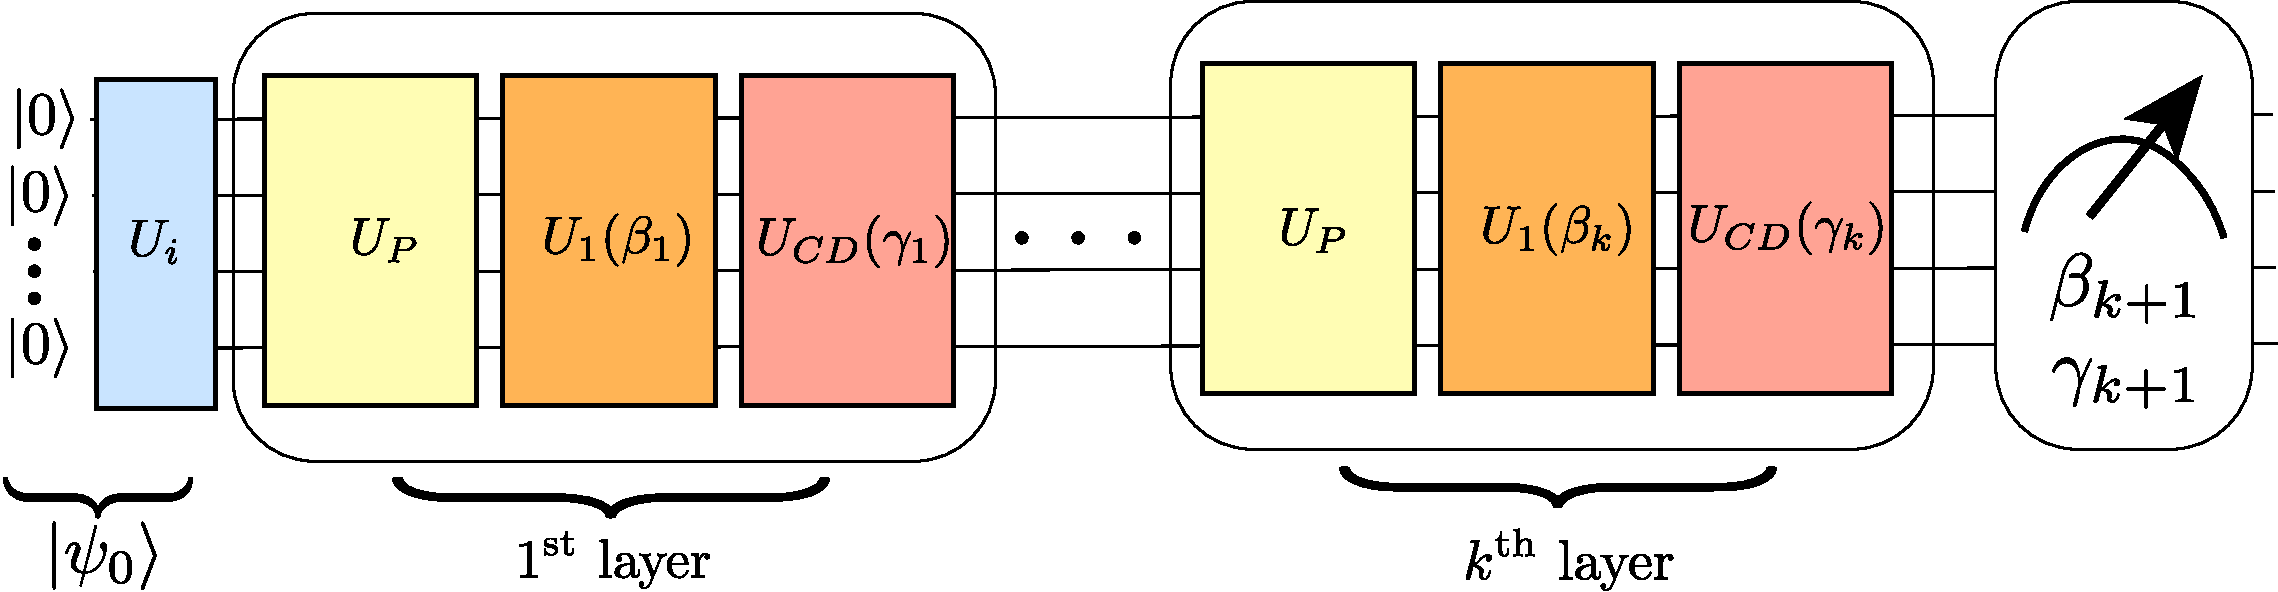
\includegraphics[scale=0.4]{Circuit.pdf}
\caption{
   The schematic diagram of the CD-FQA quantum circuit up to
   $k^{\text{th}}$ layer is shown. The  $(k+1)^{\text{th}}$
   layer is parameterized by $\beta_{k+1}$ and $\gamma_{k+1}$.
  % and are given by % related to the 
   These are obtained by measuring the respective 
   commutator expectation values % of the commutators
   $\beta_{k+1} = i\langle \psi_{k}|[H_{P}, H_{1} ]|\psi_{k}\rangle$ and
   $\gamma_{k+1} = i\langle \psi_{k}|[H_{P}, H_{\rm CD}]|\psi_{k}\rangle$.}
\label{fig:1}
\end{figure*}
%%%%%%%%%%

This work presents a significant enhancement to the FQA through
the integration of the counterdiabatic driving
protocol~\cite{demirplak2003adiabatic}, formally termed the
Counterdiabatic Feedback-Based Quantum Algorithm (CD-FQA). While
FQA draws upon QLC principles, counterdiabaticity, a concept
derived from adiabaticity, is employed to effect rapid changes
in the time-dependent Hamiltonian without inducing nonadiabatic
transitions. The utilization of counterdiabaticity in quantum
circuits has been previously applied within the framework of VQA~\cite{yao2021reinforcement,chandarana2022digitized}. Here, we
explore the dynamic interplay between QLC and
counterdiabaticity, applying these principles to the design of
quantum circuits for the ground-state preparation of
Hamiltonians representing one-dimensional (1D) Ising model
Hamiltonians. Distinct from FQA, each layer in CD-FQA includes a
third unitary inspired by the counterdiabatic driving protocol, see Fig.~\ref{fig:1}.
This addition results in a notable reduction in depth compared
to the standard FQA. The selection of the third unitary is
performed from a pool of counterdiabatic operators. It is
demonstrated that an improper choice from this pool can lead to
convergence issues in the dynamics. The implications of these
findings are discussed in the context of advancing quantum
algorithms for ground-state preparation.

% \hongye{Methods using the evolution of quantum states are introduced to prepare the ground state approximately, such as quantum adiabatic algorithm\cite{farhi2000quantum} and quantum annealing\cite{kadowaki1998quantum}. Other methods using hybrid classical optimization and quantum evaluation, such as quantum approximate optimization algorithm (QAOA)\cite{QAOA} and variational quantum eigensolver (VQE)\cite{peruzzo2014variational}, have not yet proved any quantum advantage for general cases, but may have better performance over classical counterparts for combinational problems\cite{zhou2020quantum} and quantum chemistry\cite{peruzzo2014variational}.}
% \\
% \raj{2.Feedback-based quantum algorithm and Lyapunov control}
% \hir{2.X. Magann et al. followed up on FALQON, showing that a randomized operator pool can be useful to evade vanishing gradient in the energy decrease, although generically this may require an exponentially large size of the operator pool. It would be therefore useful to have some guiding principle on what types of operators lead to efficient energy decreases.}
% \\
% \raj{3.In this paper:}
% \\



%Feedback-based quantum algorithms are often utilized to design quantum circuits that describe controlled time-evolutions of any given quantum state. 
% The control parameters are obtained by m


% layer-by-layer, where a new layer containing unitary operators is added to a previously built circuit.  
%a discretized time-evolution of the quantum state----------------------------------------------

The article is structured as follows:
\Sec{sec:QLC} %  Section II 
provides a review of QLC, while 
\Sec{sec:CD} % Section III 
establishes a connection
between the counterdiabatic driving protocol and QLC, exploring
the selection of the second control Hamiltonian for the CD-FQA.
In \Sec{sec:CD-FQA} % Section IV, 
we present the CD-FQA, comparing complexities
with the standard FQA. \SEC{sec:results:Ising} % Section V 
applies the CD-FQA to diverse
Ising models and discusses the outcomes. 
\SEC{sec:experiment} % Section VI 
demonstrates the implementation of CD-FQA on cloud quantum computers.
\SEC{sec:discussion} % Section VII 
discusses various implications of CD-FQA, and the conclusion is presented
in \Sec{sec:conclusion}. % Section VIII.

\section{Quantum Lyapunov control}
\label{sec:QLC}

Quantum Lyapunov Control (QLC) represents a form of quantum
control engineered to guide a quantum system from an arbitrary
initial state, denoted as $\vert \psi_i \rangle$, to a specified
final state, $\vert \psi_f \rangle$. This steering process is
facilitated by a target-specific control function $V(t)$,
referred to as the Lyapunov function. The design of such
controlled dynamics often involves placing constraints on the
Lyapunov function.

Consider, for instance, the task of preparing the ground state
of a many-body system for a given  % with the
physical or {\it problem} Hamiltonian $H_P$.
In cases where
the ground state is initially unknown, the system's energy
$E_P(t) = \langle \psi(t) \vert H_P \vert \psi(t) \rangle
\equiv \langle H_P \rangle_t$
naturally emerges as a suitable Lyapunov function. The
controlled dynamics is formulated to adhere to the constraint
$\frac{d}{dt}E_P \equiv \dot{E}_P \leq 0$, 
ensuring that at each time step, the system's
energy experiences a decrement. This condition guarantees a
systematic reduction in the system's energy as the controlled
evolution unfolds.

Let us begin with a driven quantum system, where the dynamics
is governed by the Schr{\" o}dinger equation
\begin{equation}
    i\tfrac{d}{dt}|\psi(t)\rangle
  = \left(H_{P}+H_{C}(t)\right)|\psi(t)\rangle,
\label{Schrodinger}
\end{equation}
where $H_P$ is the problem Hamiltonian as above, and
$H_C(t)$ is the {\it control Hamiltonian}. For convenience, we
set $\hbar=1$, throughout. % to unity.
The control Hamiltonian $H_C(t)$ % , in general, 
can be expressed in the general form
\begin{equation}
H_C(t)=\sum_{m=1}^{M} \beta_{m}(t)H_{m}.
    \label{ctrl-ham}
\end{equation}
In this formulation, the $H_m$'s represent $m=1,\ldots,M$ % the 
time-independent Hermitian {\it mixing} operators, 
with % and 
the time-dependence % is 
embedded in the
real-valued control fields $\beta_m(t)$. 
% The critical selection of 
These control parameters are chosen such that they
ensure a negative rate of change of the % average 
energy $E_P(t) \equiv \langle H_P \rangle_t$
of the problem Hamiltonian, % given by:
\begin{eqnarray}
   \tfrac{d}{dt}E_P(t)
 &=& i\langle [H_{C},H_{P}] \rangle _t
 \label{EP-dot} \\
 &=& \sum_{m}\beta_m(t) \underbrace{
   i\langle [H_{m},H_{P}] \rangle _t}_{\equiv A_m(t) \ \in\ \mathbb{R}}
   \equiv \boldsymbol{\beta}(t) \cdot {\bf A}(t)
 \ \leq\ 0
\text{ ,}\notag
\end{eqnarray}
with real-valued $M$-dimensional vectors $\boldsymbol{\beta}$ and $\bf A$
in the last expression, and expectation values are obtained
with respect to the wavefunction $\psi(t)$.
To ensure negative
$\dot{E}_P(t) \leq 0$, the conventional choice for the control field is used
$\boldsymbol{\beta}(t) = - \alpha {\bf A}(t)$
with $\alpha>0$. We note that when the system size, $N$, increases the expectation value of commutators $A_{m}(t)$ increases linearly with system size. Therefore, to keep the protocol system independent, we choose 
\be
     \boldsymbol{\beta}(t)
  = -\alpha \,  \tfrac{1}{NJ^2} {\bf A}(t)
\text{ ,}\label{alpha}
\ee
where we applied a factor $1/J^2$
on the r.h.s. to make both, $\alpha$ and $\beta$ dimensionless, and $J$ is the energy scale of the system.
% AW: By Eq. 2, beta must be dimensionless;
% the way A is defined though, it carries units E^2
Then, each protocol can be defined by a fixed $\alpha$ that is
independent of the system size.


While usually $M=1$,
the QLC method seamlessly extends to scenarios involving
multiple control fields, $M>1$. 
The inclusion of additional parameters therefore emerges as an
intuitive approach to expedite the preparation of the target
state.
% For a single % singular 
% control field, $M=1$,  with
% % $A_1(t)\equiv i\langle \psi(t)|[H_{1},H_{P}]|\psi(t)\rangle$.
%   $A_1(t)\equiv i\langle [H_{1},H_{P}]\rangle _t$,
% it holds that ${\dot E}_P =\beta_1(t)A_1(t)$.
% The condition ${\dot E}_P \leq 0$ is satisfied when
% $\sgn \beta(t)=-\sgn A_1(t)$. The conventional choice for the
% control field is $\beta(t)=-\alpha A_1(t)$ with % , where 
% $\alpha>0$ which % . This
% guarantees % that the rate of change of energy is 
% \mbox{$\dot{E}_P =-\alpha A_1(t)^2 \geq 0$}.
The Lyapunov function, derived from the solution
of \Eq{Schrodinger}, converges to the minimum of $E_P(t)$
under specific sufficient conditions \cite{grivopoulos2003lyapunov,
QLC_Beauchard_2007, QLC_Zhao_2012, QLC_Wang_2013}. Furthermore,
the state converges to a set of states characterized by La
Salle’s invariance principle \cite{la1976stability}.

% The QLC method seamlessly extends to scenarios involving
% multiple control fields. 
% There with
% % $A_m(t)\equiv i\langle \psi(t)[H_{m},H_{P}]|\psi(t)\rangle$.
%   $A_m(t)\equiv i\langle [H_{m},H_{P}]\rangle _t$,
% the % strategic selection of
% control fields are still selected such
% that they maintain % is pivotal to maintaining 
% a negative sum
% % There the rate of change of average energy becomes % is denoted as 
% ${\dot E}_P =\sum_{m}^{M}\beta_m(t)A_m(t) \leq 0$. 
% % a negative overall summation. 
% A straightforward extension from the conventional
% choice for a single control field to multiple control fields
% results in $\beta_{m}(t)=-A_{m}(t)$, ensuring an
% enhanced decrease of the energy. % negative total summation.
% The inclusion of additional parameters therefore emerges as an
% intuitive approach to expedite the preparation of the target
% state.

In the subsequent section, we demonstrate that these additional
control fields can be derived from a pool of operators commonly
employed in the context of the counterdiabatic driving protocol.
This methodology presents a promising avenue for
enhancing the efficiency of state preparation using a QLC protocol.


\section{Counterdiabatic drive inspired control Hamiltonians}
\label{sec:CD}

The counterdiabatic driving protocol is a pivotal concept in
non-equilibrium physics, employed to induce
rapid changes in the time-dependent Hamiltonian without inducing
transitions \cite{demirplak2003adiabatic,sels2017minimizing}
across instantaneous eigenstates.
This phenomenon is also recognized as a ``shortcut to
adiabaticity" \cite{chen2010fast, del2013shortcuts,
guery2019shortcuts,takahashi2019hamiltonian}. 


Consider a time-dependent Hamiltonian $H(\beta(t))$, where
$\beta$ represents an arbitrary function of time. When a quantum system, initially prepared in an eigenstate of the initial Hamiltonian, evolves
under $H(\beta(t))$, it undergoes nonadiabatic excitations,
causing it to deviate from the instantaneous eigenstate. To
eliminate such transitions, a velocity-dependent term
proportional to $\dot{\beta}$ is introduced to the original
Hamiltonian, yielding $H(\beta)+\dot{\beta} A_{\beta}$.
Here, $A_{\beta}$ is defined as
\begin{equation}
\langle m|A_{\beta}|n\rangle=i \langle m|\partial_{\beta} n\rangle=-i\frac{\langle m|\partial_{\beta} H | n\rangle}{\epsilon_{m}-\epsilon_n},
    \label{gaugepotential}
\end{equation}
is known as adiabatic gauge potential
with $|n\rangle$ the instantaneous eigenstates of $H(\beta(t))$.


Finding an exact form of $A_{\beta}$ for many-body quantum
Hamiltonians is impractical since it requires diagonalizing the
time-dependent many-body Hamiltonian. However, recently it has been shown in Ref.~\cite{PolkovnikovPRL2019}
that an approximate gauge potential can be obtained without the
need for diagonalization. This approximation is constructed
using % a
nested commutators, % defined as follows:
\begin{equation}
  A_{\beta}^{l}=i\sum_{k=1}^{l} \gamma_{k}(t) \underbrace{[H(\beta),[H(\beta),...[H(\beta)}_{2k-1~{\text{times}}},
  \underbrace{\partial_{\beta} H(\beta)}_{
    \equiv H_1
  }]]
\,, \label{gauge}
\end{equation}
determined by a set of coefficients
$\{\gamma_1,\gamma_2,...,\gamma_l \}$, where $l$ is the order of
the expansion. By properly tuning these coefficients one can suppress the nonadiabatic excitations in the system. 
As seen from \Eq{gaugepotential},
the matrix elements of the counterdiabatic operator
$\hat{A}$ change sign when taking the transpose.
For real matrix elements $\langle m|\partial_{\beta} H | n\rangle$, 
the operator $\hat{A}$ is antisymmetric and purely imaginary.
 In this case (relevant for our work here) only odd nested commutators are \cite{PolkovnikovPRL2019}
included in \Eq{gauge}.
% the nested commutator generates imaginary operators, and
For large values of $l$, the gauge
potential incorporates long-range interacting terms. In cases
where the physical Hamiltonian encompasses terms up to
nearest-neighbor interactions, it may be possible %{\color{red} feasible or possible?} 
to approximate the
adiabatic gauge potential solely with local and two-body
interaction terms \cite{vcepaite2023counterdiabatic}.

% Up to the second order in the expansion of the nested commutator $l=2$, one can generate an operator pool  \textcolor{red}{[tcw: you already assume the Ising Hamiltonian?]} [\raj{TO be removed}]
% \begin{equation}
% A=\{\sigma^y, \sigma^z \sigma^y, \sigma^y\sigma^z,\sigma^x\sigma^y,\sigma^y\sigma^z
% \}
%     \label{pool}
% \end{equation}
% These operators include a single $\sigma^y$. Note that higher-order operators include an odd number of $\sigma^y$'s. 

Having reviewed the counterdiabatic driving protocol, we now apply it in the context of QLC, where we introduce additional control fields inspired by counterdiabatic driving protocols.  This inspiration is only in spirit and stems from the fact that the imaginary operators computed from Eq.~(\ref{gauge}) can generate fast mixing between different eigenstates. However, we note that our goal is not to make the system adiabatic. Rather, we propose to find the coefficient $\gamma_{k}(t)$ using multi-control QLC. Then, the resulting $A_{\beta}^{l}$ may not be truly a gauge potential. The main idea here is to use the operators from the nested commutators and the coefficients from the QLC and integrate them into the quantum circuit. 

% {\color{red} I am a bit confused by this sentence.  If you want to induce transitions between eigenstates isn't this the opposite of want counterdiabatic drives are meant to achieve?  Don't you want the CD term to allow you to follow the instantaneous eigenstate?}

The time-dependent Hamiltonian including the first control field 
\begin{equation}
   H(\beta(t)) % {\cal H}(t)
   % not \cal for consistency with other parts of the paper
   % also pretty much the only place here that uses \cal H?
   = H_P+\beta(t) \,H_1 \ ,
\label{Ham-one}
\end{equation}
where $\beta \equiv \beta_1$ is the control field
that takes the role of $\beta$ earlier. The time evolution mixes the eigenstates of $H_P$, with couplings $\langle n|H_1|m\rangle$ between the $n^{\text{th}}$ and $m^{\text{th}}$ levels. The first control Hamiltonian is chosen heuristically. To enhance population transfer, it is essential to devise a dynamic process that facilitates swift mixing between
instantaneous eigenstates and surpasses % , surpassing
the efficiency of the QLC
with a single control parameter. To address this, we incorporate
an additional control Hamiltonian into the feedback algorithm.
While the potential addition of any number of control
Hamiltonians are feasible in principle, our preference is to
limit it to one due to the practical considerations associated
with quantum circuit implementations. 


% By expressing the wavefunction 
% $|\psi(t)\rangle=\sum_n % {n=0}^{{\cal N}-1}   % AW
% % AW: {\cal N} not defined; not really necessary to introduce?
% a_{n}(t)|n\rangle$
% in the full eigenbasis
% % $H_P=\sum_n % {n=0}^{{\cal N}-1} % AW
% % \epsilon_n|n\rangle \langle n|$, 
% $H(t) |n(t) \rangle = \epsilon_n(t) |n(t)\rangle$
% of the problem Hamiltonian,
% %Assuming the eigen energies are ordered as $\epsilon_0<\epsilon_1<...\epsilon_{{\cal N}-1}$, 
% the Schr{\"o}dinger equation for the time-dependent Hamiltonian
% (\ref{Ham-one}) can be written as
% %
% \begin{equation}
%    i\dot{a}_n = \epsilon_n a_n
%    + \beta(t) \sum_m % {m=0}^{{\cal N}-1} % AW
%    \langle n|H_1|m\rangle \,a_m \ .
% \label{Schrodinger-amp}
% \end{equation}
% The amplitudes $a_n$ and $a_m$ are coupled to each other via
% $H^{(1)}_{nm} \equiv\langle n|H_1|m\rangle$ and $\beta(t)$ is a % global 
% scaling factor 
% applied equally % applicable  // AW
% to all terms. % couplings. 
% Initially, the system
% starts as a superposition of the eigenstates of $H_P$. The
% dynamics in (\ref{Schrodinger-amp}) describe population transfer
% between different levels, and by tuning the parameter $\beta(t)$
% according to QLC, one can find a dynamics in which the average
% energy $\la H_P \ra$ decreases towards
% % goes down and finally the system ends up at
% the ground state of $H_P$.

% % If we consider $\beta=\beta$, then the time-dependent Hamiltonian ${\cal H}(\beta(t))$ describe
% % $\beta=\beta$  

% To enhance population transfer, it is essential to devise a
% dynamic process that facilitates swift mixing between
% instantaneous eigenstates and surpasses % , surpassing
% the efficiency of the QLC
% with a single control parameter. To address this, we incorporate
% an additional control Hamiltonian into the feedback algorithm.
% While the potential addition of any number of control
% Hamiltonians is feasible in principle, our preference is to
% limit it to one due to the practical considerations associated
% with quantum circuit implementations. 

%\awc{skip the following sentence?}
% AW: what precisely do you want to say here?
%However, the selection
%criteria for this supplementary control Hamiltonian remain unclear. 

%The optimal choice depends on various factors, including the specific characteristics of the quantum system under consideration and the desired outcomes of the population transfer. Careful consideration and, possibly, numerical optimization methods may be employed to determine the most effective additional control Hamiltonian for the given scenario.

%However, it is not straightforward how one would choose these additional Hamiltonians. 

% AW: tried to shorten to the essential
% \awx{We note the presence of inherent parameters in the system,
% specifically the energy differences $\epsilon_{mn}$, which can
% be harnessed to generate additional control parameters. One
% approach is to consider the energy differences of the static
% Hamiltonian $H_P$. Alternatively, one may explore the energy
% differences of the time-dependent Hamiltonian ${\cal H}(t)$.
% Both methods offer avenues for creating supplementary control
% parameters that can be leveraged to optimize the dynamic
% processes within the system.}

%The choice between static and time-dependent energy differences may depend on the specific characteristics and requirements of the quantum system under consideration.

To speed up transitions across wider energy
intervals, one can weight transitions based on the
energy differences between instantaneous eigenstates.
Hence
% When considering the energy differences of $H_P$, equation
\Eq{Schrodinger} with an additional control Hamiltonian $H_{\rm CD}$, i.e.,
\begin{equation}
    H_P + H_C(t) = H(\beta(t))+\gamma(t)H_{CD},
\end{equation}
reads
\begin{equation}
i\dot{a}_n=\epsilon_n a_n+ \gamma(t) \sum_m % {m=0}^{{\cal N}-1} 
    \la n|H_{\rm CD} |m \ra a_m,
    \label{Schrodinger-amp1}
\end{equation}
where we have written $|\psi(t)\rangle$ as
$$
|\psi(t)\rangle = \sum_n a_n(t)|n(t)\rangle,
$$
where the $|n\ra$'s are the instantaneous eigenstates of
$H(\beta(t))$.  The matrix element $\la n|H_{\rm CD} |m \ra$
must be dependent on the energy differences between level $n$
and level $m$. We select $H_{\rm CD}$ from a pool constructed by the nested commutator
$A_{\beta}^{l}$ in Eq.~(\ref{gauge}). 
The control field
$\gamma(t)$ is determined by the QLC protocol described in
\Sec{sec:QLC}. % Section II. 






% Based on \Eq{gauge},
% % the function $f(\epsilon_{mn})$ can be expressed as
% $f(\epsilon_{mn},t) = i \sum_{k=1}^{l}\gamma_{k}(t) \,
% \epsilon_{mn}^{2k-1}$ can be expressed as a power-series in % where
% $\epsilon_{mn} \equiv \epsilon_n - \epsilon_m$.
% This function favors larger energy differences, whereas
% for processes that preserve the energy it holds that
% % and the function 
% $f(0,t)=0$.
% Again only odd powers of $\epsilon_{mn}$ are considered,
% as discussed with \Eq{gauge}.

% The energy differences in \Eq{Schrodinger-amp1}
% are based on the instantaneous eigenstates with respect to the full Hamiltonian $H(t)$ in \Eq{Ham-one}.
% For practical purposes, however, we adapt this scheme by
% favoring the energy differences with respect
% the physical target Hamiltonian $H_P$, instead,
% throughout the simulation. 

The energy differences in \Eq{Schrodinger-amp1} are based on the
eigenstates of the Hamiltonian $H(\beta(t))$.  The control
Hamiltonian $H_{\rm CD}$ can also be constructed from
\Eq{gauge}, by replacing $H(\beta(t))$ with the problem
Hamiltonian $H_P$.  The operator pool generated by the nested
commutator constructed from $H_P$ is a subset of the operator
pool generated by Eq.~(\ref{gauge}). For practical purposes, one
can use both sets of operator pools. Since we strongly truncate
the series in \Eq{gauge} anyway, we expect both pools to have
comparable performance. 

% We also highlight that operators generated by 

%  This limitation stems from the fact that Eq. (\ref{nested-comm}) considers the energy differences between static levels, while Eq. (\ref{gauge}) incorporates the energy differences between the instantaneous eigenenergies of ${\cal H}(t)$ when setting $\beta=\beta$. The distinction in the considerations of energy differences results in a more constrained set of operators for Eq. (\ref{nested-comm}).


% \awc{skip the rest of this section?}
% The function $f$ can
% be written as $f=f_{\text{even}}+f_{\text{odd}}$, where even and
% odd refer to the even and odd powers of $\epsilon_{mn}$,
% respectively. The function $f_{\text{odd}}$ must be imaginary so
% that the Schr{\"o}dinger equation describes a Hermitian
% time-dependent Hamiltonian. The function $f_{\text{odd}}$ has
% the following form
% \begin{equation}
% f(\epsilon_{mn},t)=i\sum_{k=0}^{l}\gamma_{k}(t) (\epsilon_{mn})^{2k-1},
%     \label{function-1}
% \end{equation}
% here $\gamma_k(t)$ are real valued. The operators that can generate such a coupling is 
% \begin{equation}
% A_{\text{odd}}=i\sum_{k=0}^{l} \gamma_{\text{odd},k}(t) \underbrace{[H_P,[H_P,...[H_P}_{2k-1~{\text{terms}}},H_1]]
%     \label{nested-comm}
% \end{equation}
% Remarkably, equation (\ref{nested-comm}) shares the same form as the approximated gauge potential in Eq. (\ref{gauge}) \cite{PolkovnikovPRL2019}. Moreover, the expression for operators that generate $f_{\text{even}}$ is given by:
% \begin{equation}
% A_{\text{even}}=\sum_{k=0}^{l} \gamma_{\text{even},k}(t) \underbrace{[H_P,[H_P,[H_P,...[H_P}_{2k~{\text{terms}}},H_1]]],
%     \label{nested-comm-even}
% \end{equation}
% which also includes diagonal terms.

% It's crucial to highlight that operators generated by Eq. (\ref{nested-comm}) constitute a subset of the operator set generated by Eq. (\ref{gauge}). Consequently, Eq. (\ref{nested-comm}) imposes more restrictions and encompasses a smaller number of operators compared to the latter. This limitation stems from the fact that Eq. (\ref{nested-comm}) considers the energy differences between static levels, while Eq. (\ref{gauge}) incorporates the energy differences between the instantaneous eigenenergies of ${\cal H}(t)$ when setting $\beta=\beta$. The distinction in the considerations of energy differences results in a more constrained set of operators for Eq. (\ref{nested-comm}).


%%%

\section{Counterdiabatic feedback-based quantum algorithm (CD-FQA)}
\label{sec:CD-FQA}

We enhance the FQA by introducing an additional control field inspired by counterdiabatic driving protocol. The resulting digital
quantum circuit for counterdiabatic FQA (CD-FQA) 
discretizes the
time evolution of the Schr\"odinger equation (\ref{Schrodinger}) with two control fields,
\begin{equation}
  i\tfrac{d}{dt}|\psi(t)\rangle
  = \bigl(
       H_P + \beta(t) H_1 + \gamma(t) H_{\rm CD}
    \bigr)|\psi(t\rangle)
\text{ ,}\label{Schrodinger-CD}
\end{equation}
where $H_{\rm CD}$ is an operator selected from the pool of
operators inspired by counterdiabatic driving protocol. 
% To be specific, $H_{\rm CD} \sim i [H_P,H_1]$ is chosen from the pool
% of operators that consist of subsets of operators generated by
% the commutator $[H_P,H_1]$.
\EQ{Schrodinger-CD} can be seen as specialization
of \Eqs{Schrodinger}-\eqref{EP-dot} for $M=2$,
with $\gamma \equiv \beta_2$ and $H_{\rm CD}$
a particular choice for $H_2$ motivated from 
counterdiabatic driving.

The CD-FQA quantum circuit is assembled by successively applying
three unitaries,
\begin{equation}
   |\psi_{l}\rangle
   =\prod_{k=1}^l {\cal U}_k|\psi_{0}\rangle
   =\prod_{k=1}^l U_{\rm CD}(\gamma_k) U_1(\beta_k)  U_{P}|\psi_{0}\rangle
\,,\label{Falqon-1}
\end{equation}
Here, $|\psi_{0}\rangle$ represents the arbitrary initial state,
$|\psi_{l}\rangle$ is the quantum state after applying $l$
layers of unitaries, and each layer is parameterized by
$\{\beta_k,\gamma_k\}$. The unitaries are defined as $U_{P}\equiv
e^{-iH_{P}\Delta t}$, $U_{1}(\beta_{k})\equiv
e^{-i\beta_{k}H_{1}\Delta t}$, and $U_{\rm CD}(\gamma_{k})\equiv
e^{-i\gamma_{k}H_{\rm CD}\Delta t}$. For small $\Delta t$, this
evolution closely resembles the
continuous-time evolution of the system. The parameter $\Delta t$
must be small enough so that the first-order reduction in
energy must exceed all the higher-order terms
\cite{FeedbackPRA}. The parameters $\beta_{k}$ and $\gamma_{k}$
for the $k^{\text{th}}$ layer are not known a priori,
as they depend on the history. They are
obtained by measuring the commutators $i\langle [H_{1},
H_{P}]\rangle$ and $i \langle [H_{\rm CD}, H_{P}]\rangle $
in a quantum circuit for the prior state
$|\psi_{k-1}\rangle$. The measurement results are then utilized
to parameterize the $k$-th layer. We adhere to the conventional
choice for the application of QLC, thus assigning the control
fields (cf. \Fig{1}):
\begin{eqnarray}
   \beta _{k+1} &=& \tfrac{i\alpha}{N}\,\langle \psi_{k}|[H_{P}, H_{1}\ \ ]|\psi_{k}\rangle, \\
   \gamma_{k+1} &=& \tfrac{i\alpha}{N}\,\langle \psi_{k}|[H_{P}, H_{\rm CD}]|\psi_{k}\rangle
\text{ .}
\end{eqnarray}
The expectation
value of an operator $\langle {\hat O}\rangle=\sum_{i}^N\!
\gamma_i\, \la {\hat P}_{i}\ra$ can be obtained by performing
measurements of the Pauli operators $P_i$.  Upon a sufficient
number of measurements, one can calculate the expectation
value. The number of Pauli operators and the number of
measurements will depend on the structure of $H_P$, $H_1$ and
$H_{\rm CD}$, which can be effectively implemented using
parallelization techniques \cite{gokhale2019minimizing,
verteletskyi2020measurement, reggio2023fast, anastasiou2023really,
 zhu2023optimizing}. 
 
 %\awc{hows this actually measured
% in the experimental circuit setting? was an auxilliary
% used for this?}

Each layer in CD-FQA comprises two parameters. In comparison
with standard FQA, % it is noteworthy that 
CD-FQA demands twice
the number of measurements per layer. The circuit depth in
CD-FQA is $3l$, while the circuit depth in FQA is only $2l$,
where $l$ is the number of layers. This extended depth per layer
reflects the added complexity introduced by the counterdiabatic
control field, emphasizing the need for enhanced computational
resources per each layer in CD-FQA. Nevertheless, the
incorporation of an additional control field in CD-FQA leads to
a reduced number of layers in CD-FQA. For a small number of
layers our algorithm shows tremendous improvement over standard
FQA.

% The advantage of using the feedback-based quantum algorithm is that the entire computation is fully quantum and does not need classical optimization. However, the algorithm is not effective for the NISQ devices, since it requires a deep circuit. Nevertheless, the FALQON algorithm is important in the sense that it can be used to initialize the parameters in QAOA. The main goal of this paper is to improve the FALQON algorithm. There are three knobs in the FALQON algorithm. They are the control fields, the control Hamiltonians, and the initial state. Here we show that the FALQON algorithm can be accelerated by using additional control Hamiltonians inspired by counterdiabatic driving. In our approach, each layer will consist of at least three unitaries $U_P$, $U_C$, and $U_{\rm CD}$. The total number of unitaries in our circuit $\sim 3k$ compared to FALQON where the number of untaries $\sim 2k$. We find a significant improvement over the FALQON, and our algorithm does not require a classical optimization and shows tremendous improvement over a small number of layers.


\begin{figure}[tbh!]
\begin{center}
  \sidesubfloat[]{\label{:a}%
  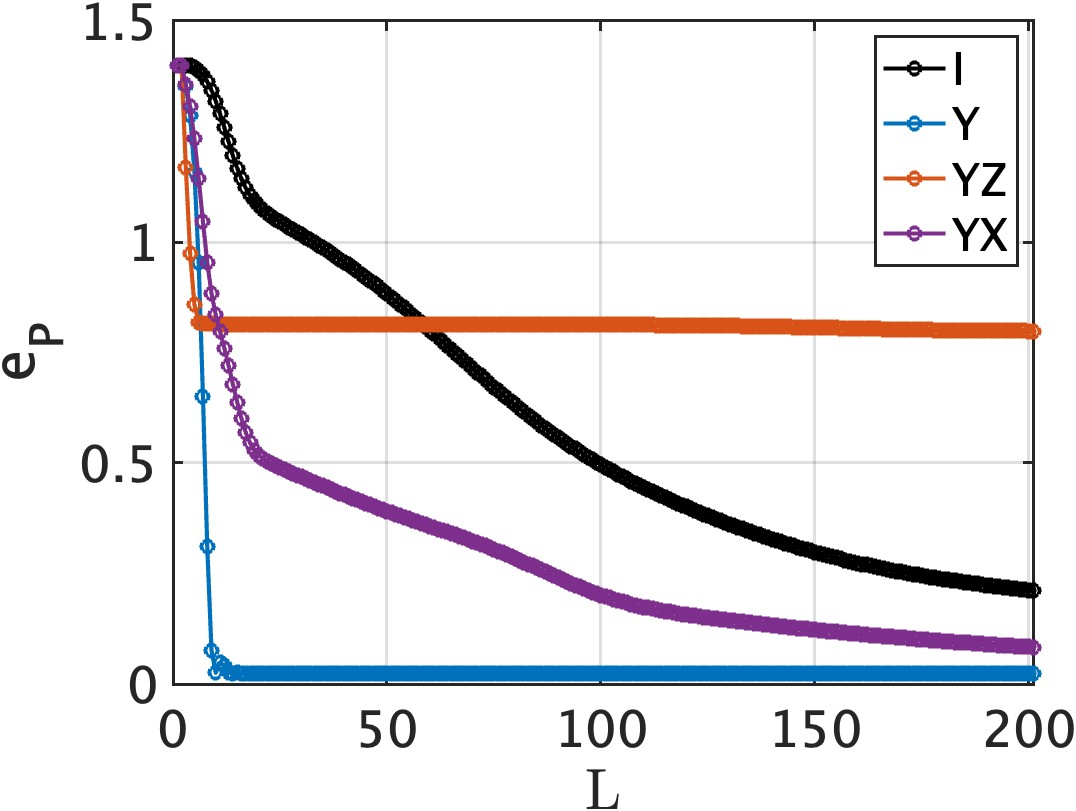
\includegraphics[scale=0.18,trim = 0in 1.5in 0in 0in, clip=true]{LFIM.jpg}} \\
  \sidesubfloat[]{\label{:b}\ \ %
  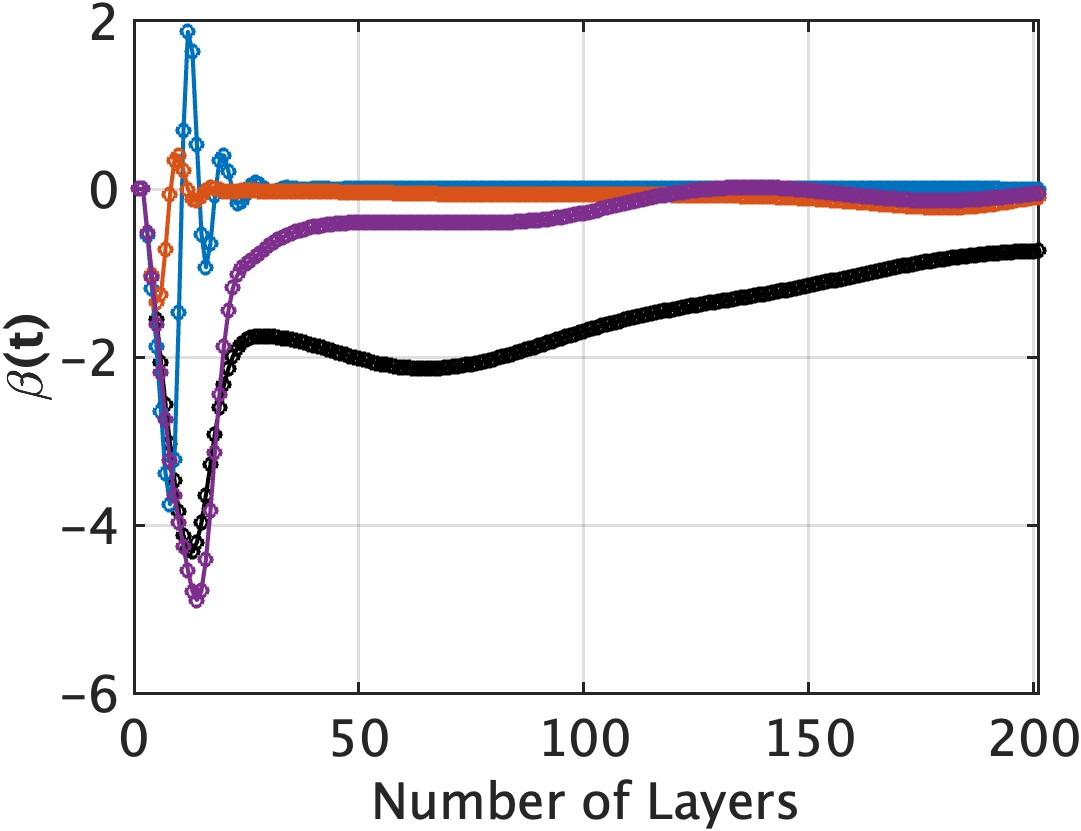
\includegraphics[scale=0.172,trim = 0in 1.6in 0in 0in, clip=true]{LFIM1040_beta.jpg}} \\
  \sidesubfloat[]{\label{:c}%
  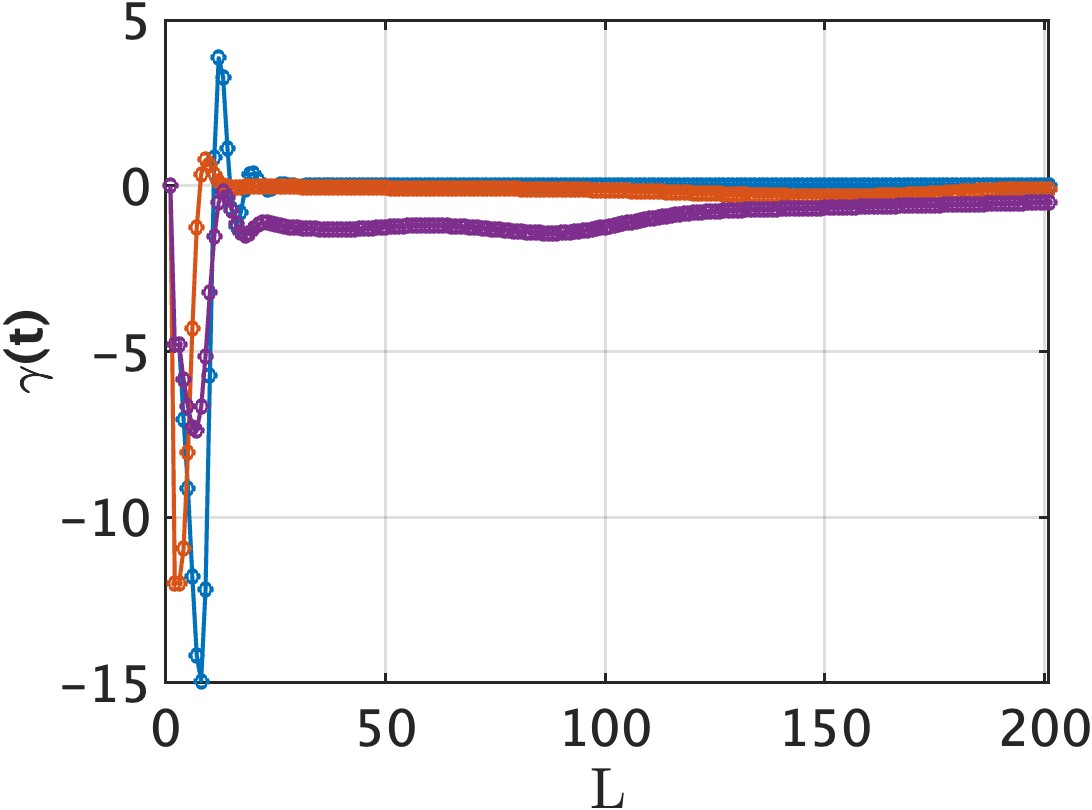
\includegraphics[scale=0.18]{LFIM1040_gamma.jpg}}
\end{center}
\caption{
(a) The average energy per site is
    shown as a function of the number of layers for LFI 
    $(h_z=0.4$, $h_x=0)$ with $N=6$ spins for various CD-FQA protocols. The black color represents
    the standard FQA which is equivalent to taking
    the identity for $H_{\rm CD}$, i.e., $H_{\rm CD}=I$
    as indicated in the legend.
    The other colors represent CD-FQA with a
    particular operator  denoted by $H_{\rm CD}$ selected from the pool (\ref{pool}).
(b) The first and (c) the second control fields, $\beta(t)$ and
    $\gamma(t)$, respectively, are shown as a function of the
    number of layers for different $H_{\rm CD}$. Parameters $\alpha=6$
    and $\Delta t = 0.01 / J$. % $\Delta t=0.01\, J$.  // AW
}
\label{fig:LFI}
\end{figure}
%%%

%%%%%%%%%%%%%%
%%%
\begin{figure}
\centering
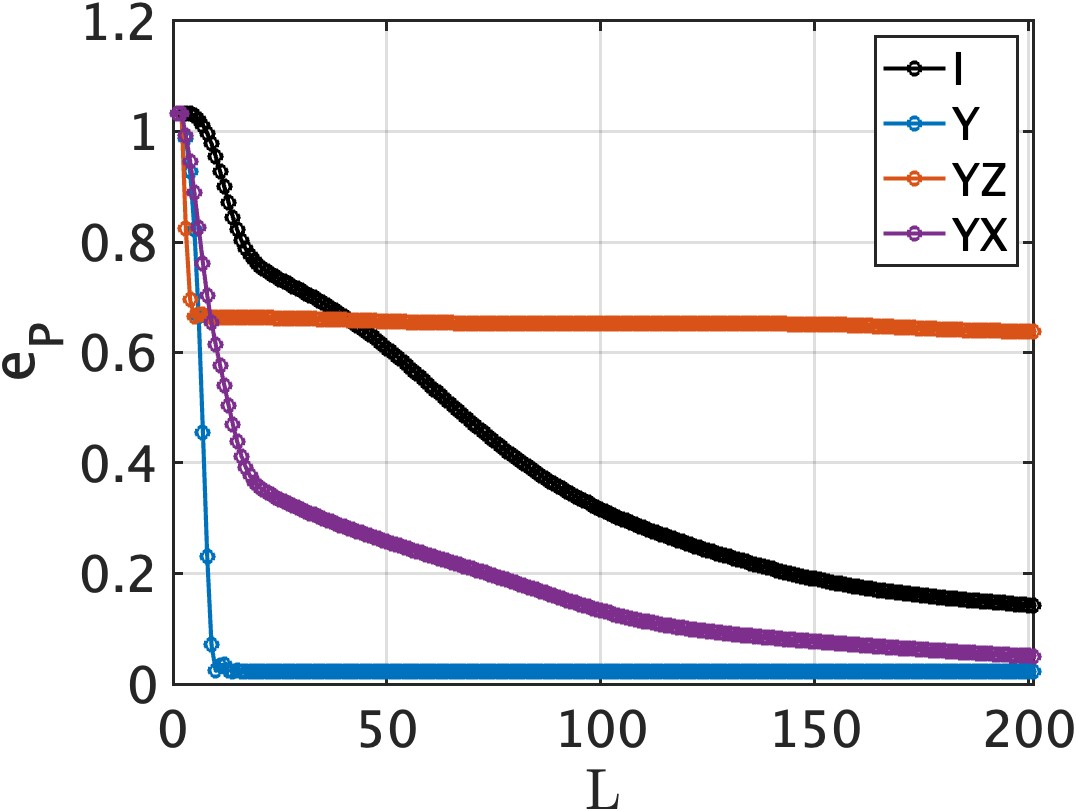
\includegraphics[scale=0.18]{MFIM.jpg}
\caption{
   The average energy per site is shown as a function of the number of
   layers for MFI ($h_z=h_x=0.4$). % , $h_x=0.4$).
   All other parameters are same as Fig. \ref{fig:LFI}.
}
\label{fig:MFI}
\end{figure}

%%%

\begin{figure}
    \centering
  % \sidesubfloat[]{\label{a}\!\!\!\includegraphics[scale=0.1]{   .jpg}\ } 
  % AW missing figure? guessing ...
    \sidesubfloat[]{\label{a}\!\!\!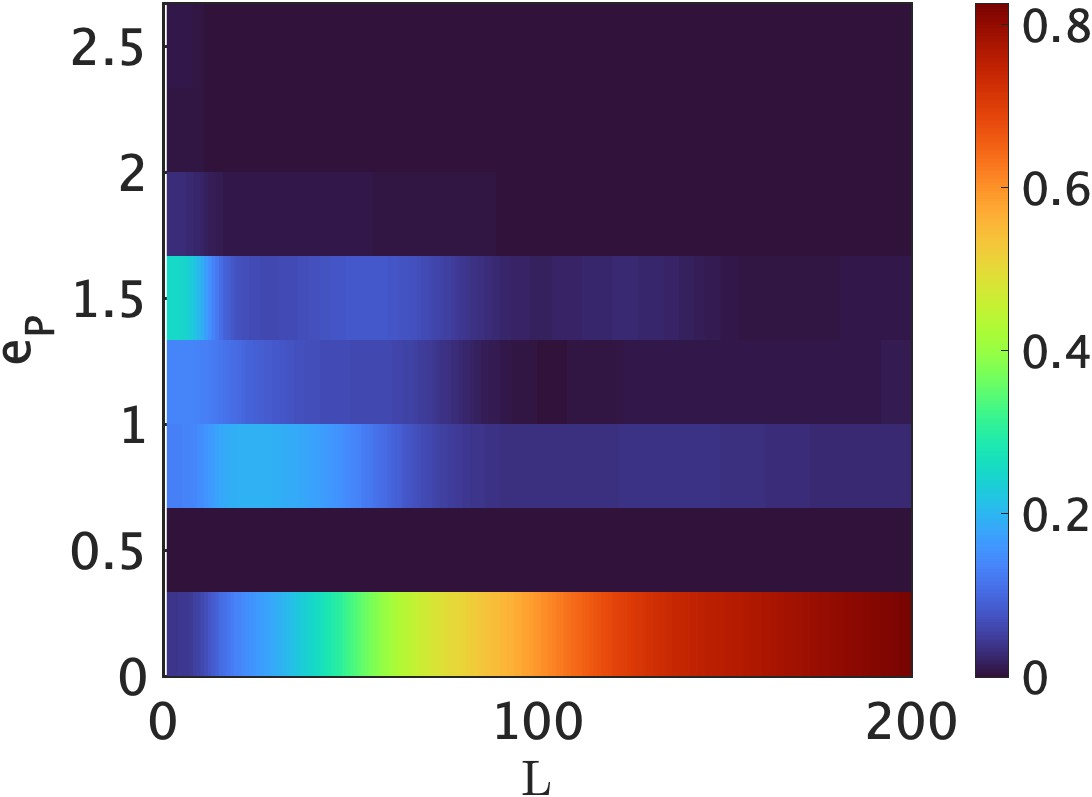
\includegraphics[scale=0.1]{3D-FQA0.jpg}\ } 
    \sidesubfloat[]{\label{b}\!\!\!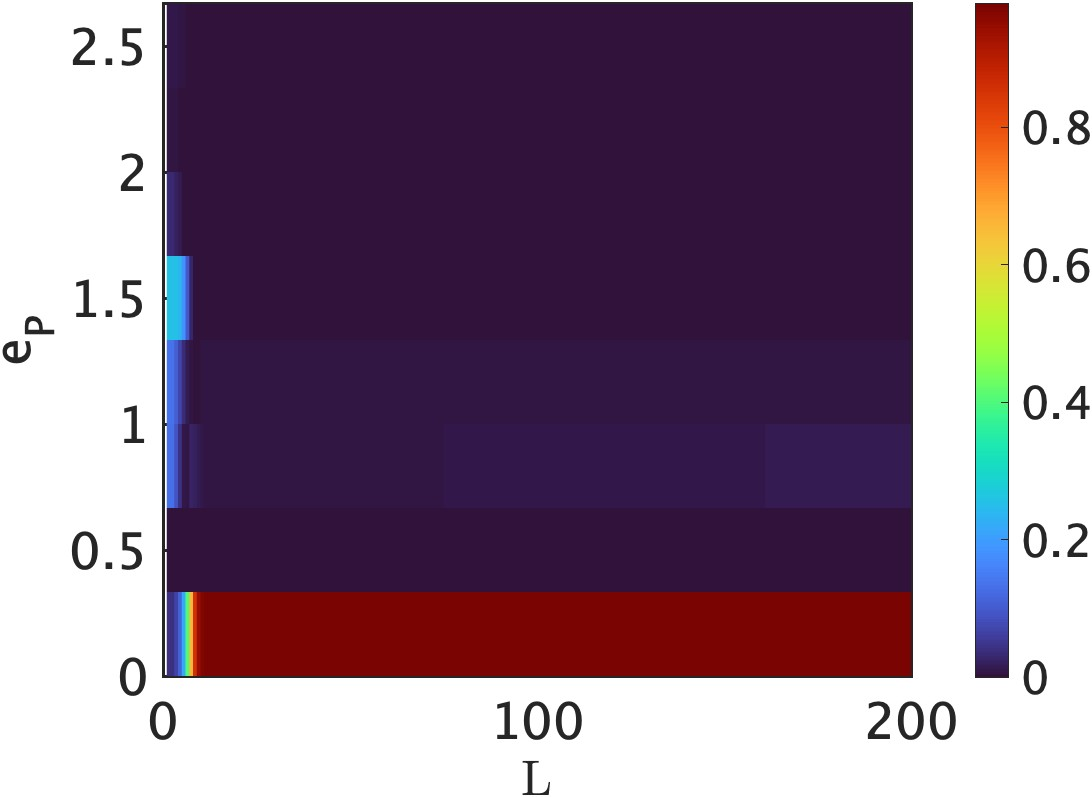
\includegraphics[scale=0.1]{3D-FQA1.jpg}}\\
    \sidesubfloat[]{\label{c}\!\!\!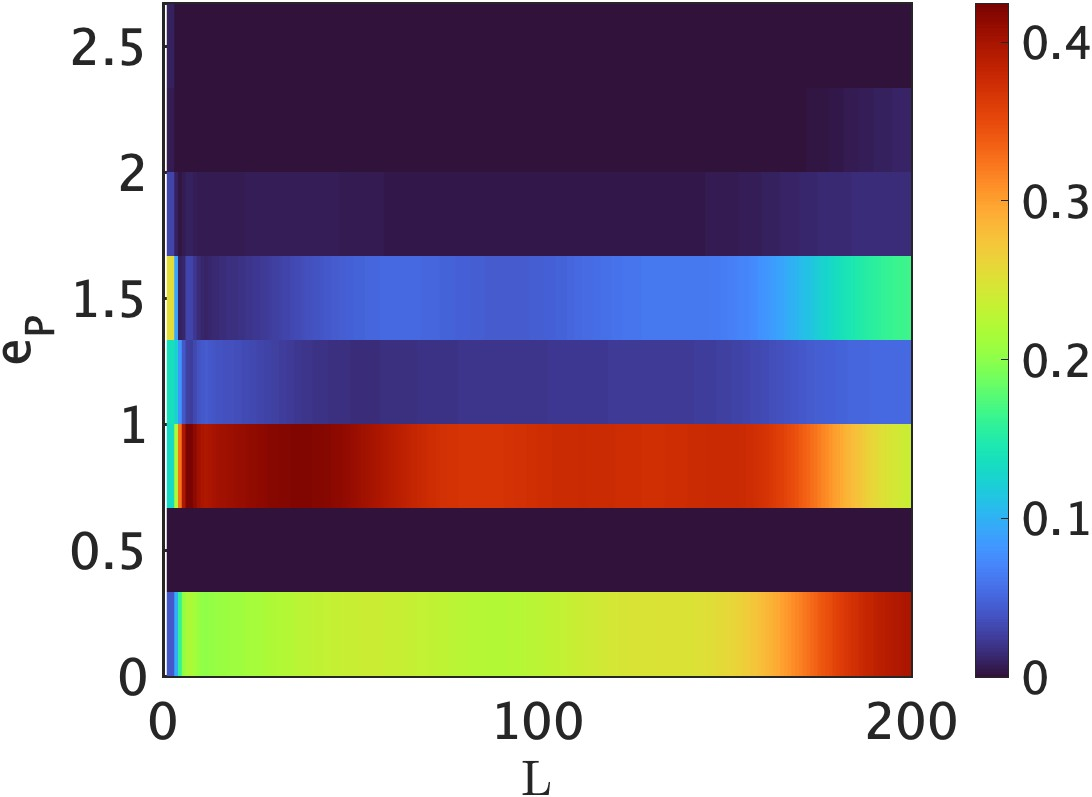
\includegraphics[scale=0.1]{3D-FQA2.jpg}\ }
    \sidesubfloat[]{\label{d}\!\!\!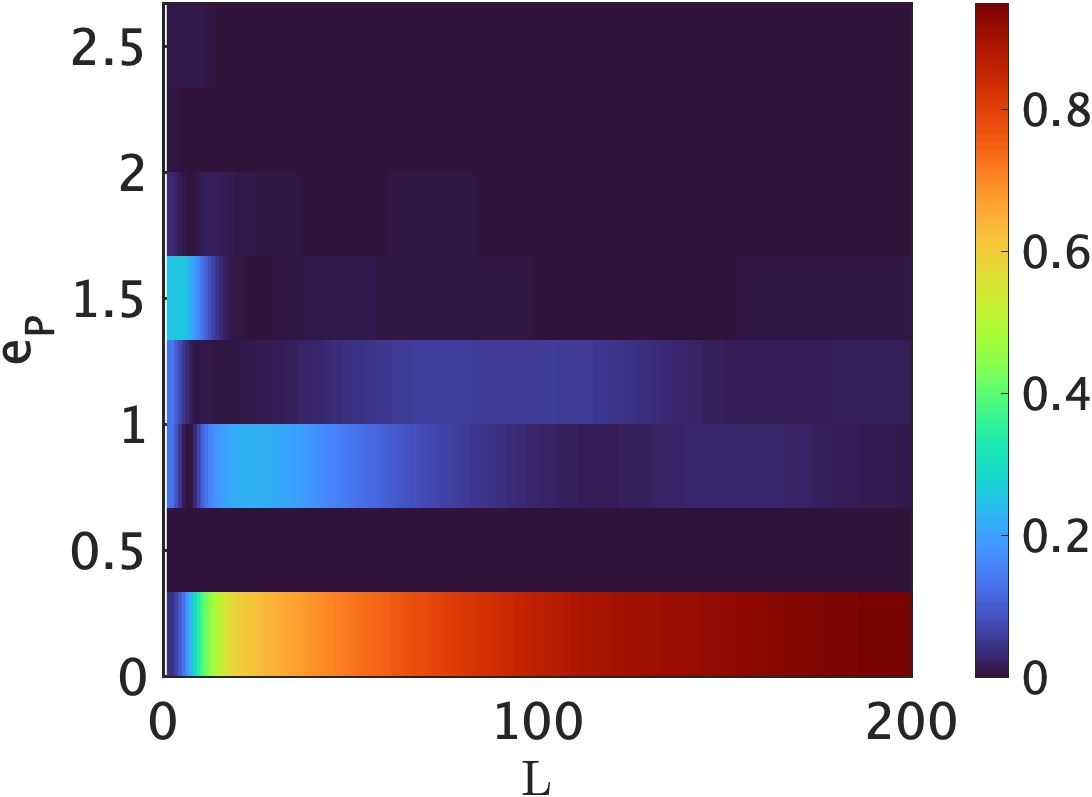
\includegraphics[scale=0.1]{3D-FQA3.jpg}}
\caption{
 % Average 
   Binned energy distribution % occupation 
   of the state $\psi$  vs. circuit depth for the MFI
   for the simulation of \Fig{MFI}.
 % of the eigenenergies of the MFI
 % Hamiltonian is shown as a function of the number of layers.
 % The parameters are the same as in  Fig. \ref{fig:MFI}, and
   The panels % color plots 
   represent CD-FQA protocols with operators
      (a) $I$ (i.e., plain FQA),
      (b) $Y$,
      (c) \YZ, and
      (d) \YX, respectively.
 % The black color corresponds to low occupation while the red color
 % represents high occupation. 
 % AW: this is apparent from the colorbar
   The average energies per site $e_P$
   are coarse-grained % put 
   into 8 bins of equal width % where each bin contains an energy range of
   $2J$. For each circuit depth,
   the energy densities integrate to $1$ vertically
   over all energies.}
\label{fig:MFIcolor}
\end{figure}
%%%

 
% %%%%%
% \begin{figure}
% \begin{center}
% 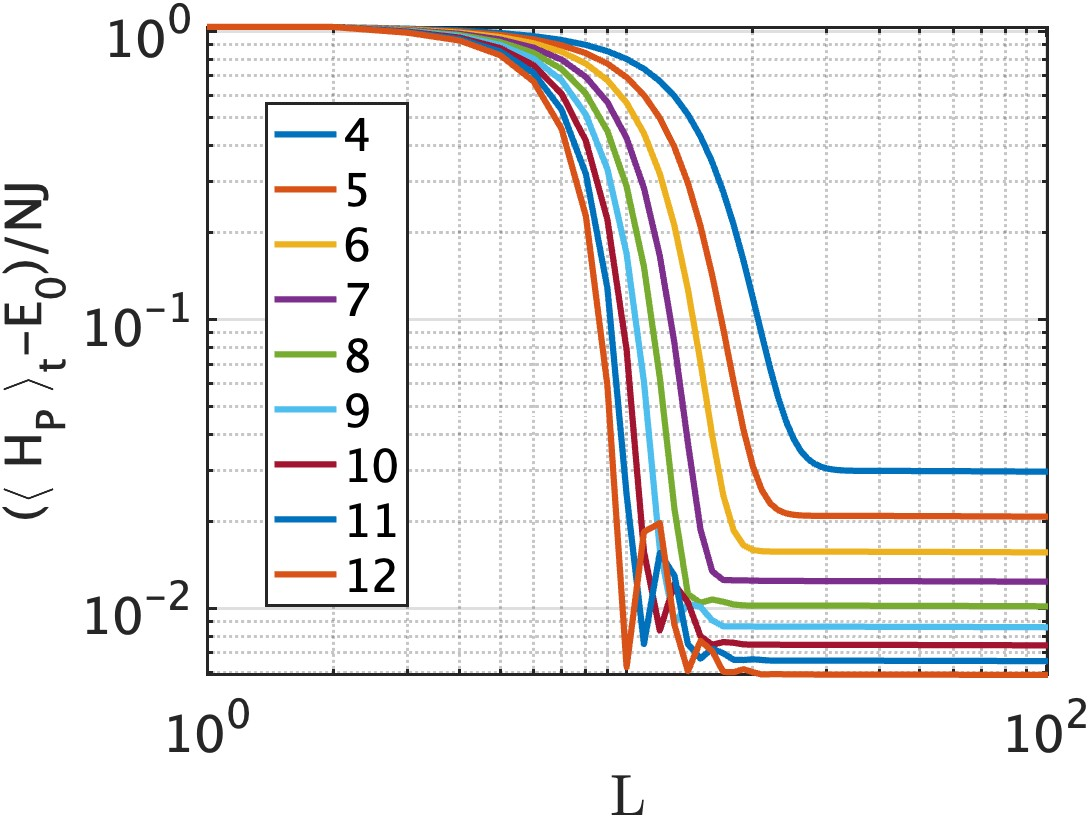
\includegraphics[scale=0.20]{MFIdifferentsize.jpg}
% 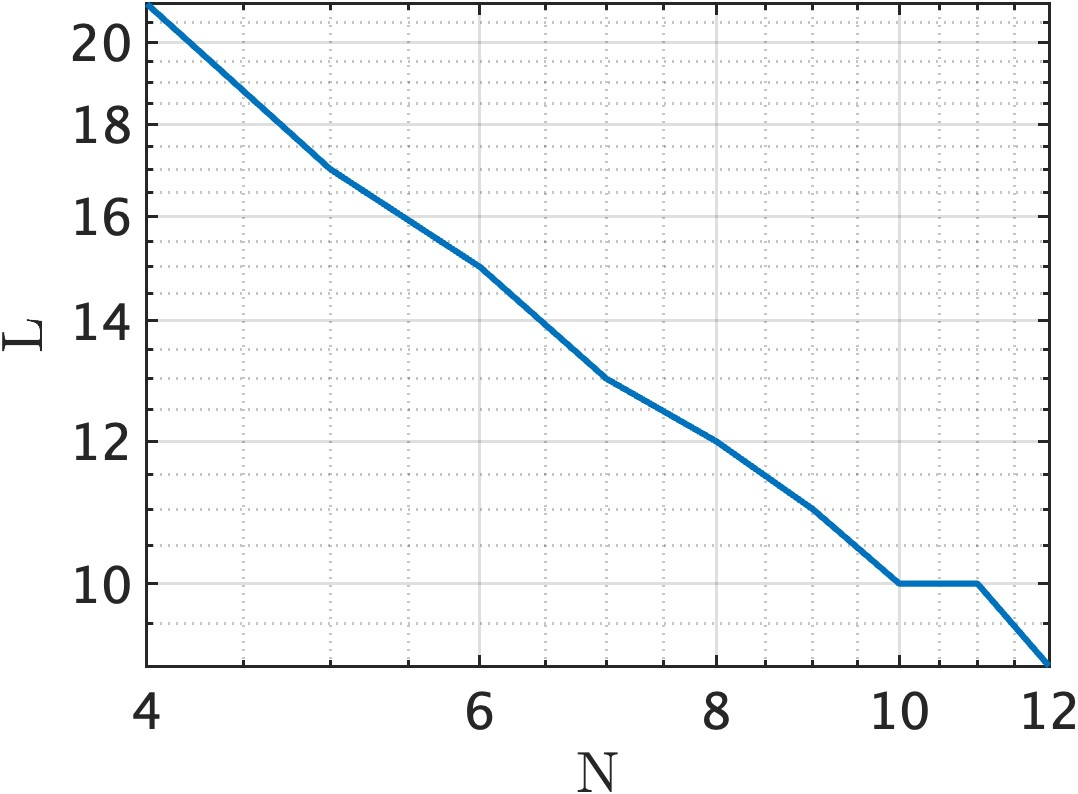
\includegraphics[scale=0.20 ]{errorplot.jpg}
% \end{center}
% \caption{ % The 
%    Average energy per site for \aw{the MFI 
%    ($h_z=h_x=0.4$, as in \Fig{MFI}, % AW check values ??
%    $\Delta t=0.005$ and $\mathcal{L} = ??$ layers)}
%    for CD-FQA protocol with $Y$ as second
%    control Hamiltonian % is shown in loglog plot for different 
%    for various system sizes \aw{$N$ as indicated in the legend}.
%    \awc{please remove `N=' in the legend}.
%     % AW: just show value; also remove box around legend?
%  % for the MFI model %. Here $\Delta t=0.005$.
%    \awc{get $n:=x$ value (number of layers)
%       where $y=0.1$, e.g., by interpolation,
%       then add panel plotting $n$ vs $N$
%       e.g. on log-log plot
%    }
%    \awc{comment on increasing energy, since by construction
%    $\dot{E}_P \leq 0$; effect of finite $\Delta t$?
%    Show results for different $\Delta t$ for one examplary case?}
% } %\hir{[HS:What are the two lowest curves for? ($N=13,14$?)]}}
% \label{fig:CDYdifferentsize}
% \end{figure}
% %%%%%

\section{Results: Preparing the ground-state of Ising spin models}
\label{sec:results:Ising}

We apply the CD-FQA to Ising chains
of length $N$  % models of the form
\begin{eqnarray}
   H_{I} % (J,h_z,h_x)
   &=& \sum_{i}^N \Bigl(
        -J \sigma_{i}^z\sigma_{i+1}^z
     - h_z \sigma_{i}^z
     - h_x \sigma_{i}^x
   \Bigr)
\label{eq:IsingModel} \\
  &\equiv& - \ZZ - h_z \, Z - h_x \, X
\text{ ,}\notag
\end{eqnarray}
and for various parameter settings.
The nearest-neighbor interaction $J:=1$ 
sets the unit of energy, throughout,
while $h_z$ and $h_x$ specify % denote the magnitudes of
 the longitudinal and transverse fields, respectively. The operators
$\sigma_{i}^a$ with $a \in \{x,y,z\}$ are the standard Pauli
operators acting on site $i$.
We use periodic boundary
conditions (PBC) in all classical simulations except for Fig. \ref{fig:experiment}
where we use open boundary conditions  (OBC) for quantum simulation.  
%
For convenience, we employ shorthand notations to describe the
sums of Pauli operators. The sum of local operators
is denoted by $A \equiv \sum_{i}^N \sigma_{i}^a$,
with $A \in \{X,Y,Z\}$ corresponding to $a\in \{x,y,z\}$, respectively.
Similarly, two-body terms are denoted by
$AB \equiv \sum_{i}^N \sigma_{i}^a\sigma_{i+1}^b$.
With this, the Hamiltonian in~\Eq{eq:IsingModel}
can be written as shown in the line below it.

By varying the parameters
%\awc{J is always 1?} % $J$, 
$h_z$ and $h_x$,
we investigate four distinct types of Ising models:
(i)   longitudinal field Ising (LFI) when $h_x$ = 0,
(ii)  transverse field Ising (TFI) when $h_z$ = 0,
(iii) mixed-Field Ising (MFI) with non-zero values for all % three
parameters, and
(iv)  A special case $h_x=h_z=0$. % where both $h_z$ and $h_x$ are zero.  
% We apply periodic boundary conditions (PBC) for
% all models, however, emphasize that these findings can readily
% extend to open boundary conditions (OBC). 
% comprehensive
This study showcases the versatility of the CD-FQA approach in
tackling various Ising models with different field
configurations. 

In all considered cases, the first control Hamiltonian is
defined as $H_1=X$. This Hamiltonian, commonly referred to as a
mixer Hamiltonian, is a standard choice in QAOA and quantum
annealing protocols, particularly when the problem Hamiltonian
consists of Z % $\sigma^{z}$ 
terms. Here, we set the initial state
to be the ground state of $-H_1$ % $H_1$:
% AW: strictly speaking, the GS of +X is |-X>
$|\psi_{0}\rangle = |X\rangle \equiv
|\rightarrow\rightarrow \ldots \rightarrow\rangle$,
where all spins
are aligned along the $x$-axis. This initial state, being a
product state, can be readily prepared on a quantum circuit
using only Hadamard gates. Equivalently,
$|X\rangle = e^{-i\frac{\pi}{4} Y} |Z\rangle$
with $|Z\rangle \equiv |{+}Z\rangle
\equiv |\uparrow \uparrow \ldots \uparrow \rangle$.

The second control Hamiltonian in our approach draws inspiration
from the counterdiabatic protocol as discussed in 
\Sec{sec:CD}, % Sec. III
and is selected from an operator pool generated by the nested
commutator Eq.~(\ref{gauge}). Importantly, we restrict
the operator pool to include only local and two-body terms. When
the problem Hamiltonian and the first control Hamiltonian are
real then the operator pool comprises solely operators with imaginary matrix elements.
%\hir{[``Imaginary operator" might be misread as an anti-hermitian operator. The operator itself is very much real.]}. 
The counterdiabatic operator pool $A_{\text{pool}}$
is a subset of the operator pool consisting of all the local and
two-body operators and is given by
\begin{equation}
   A_{\rm pool}\subseteq 
   H_{\rm pool} = \{Y, \ZY, \YZ, \XY, \YX \}
\text{ .}\label{pool}
\end{equation}
% It is straightforward to verify that certain 
The terms in \Eq{pool} are generated by commuting individual
terms of $H_P = H_I$ with $H_1=X$. As it turns out, % Note that 
\YZ and \ZY exhibit identical behavior,
similar to \YX vs. \XY. % demonstrate the same characteristics.
With this, we eliminate \ZY and \XY from the pool above.
Yet for the sake of the presentation, we include the
identity $I$ to the pool, which then simply represents
the standard FQA.
% Therefore, we present only one member from each pair for
% brevity.

\subsection{$h_z\neq 0$ (LFI and MFI)}
First, we consider the case of non-zero
longitudinal field % is non-zero,
$h_z = 0.4$ where we find that both LFI ($h_x=0$, \Fig{LFI})
%as well as 
and MFI ($h_x=h_z$, \Fig{MFI}) yield
% since the CD-FQA protocol for both models yields 
similar results.
% In Fig. \ref{fig:LFI} we present key results
% for the CD-FQA applied to the LFI with $\{ h_z,h_x\}=\{0.4,0\}$.
The system consists of $N=6$ spins, 
and the simulation is performed up to $200$
circuit layers using % and the time step is
$\Delta t=0.01$. The parameter $\alpha$ in the QLC protocol is assumed to be $6$, so that the prefactor $\alpha/N=1$. 

We depict three distinct CD-FQA protocols, each associated with
a different operator selected from the pool, characterized by
$H_{\rm CD} \in % =
\{ Y, \YZ, \YX \}$. These % operators $Y$ and \YZ 
are derived from terms that arise from
the nested commutators (\ref{gauge}),
$Y$ and \YZ at % in the
first order, and % while 
\YX at % is a 
second-order. % derivation.
The performance of CD-FQA, for each choice of $H_{\rm CD}$,
is compared against the standard FQA represented by the black
curves. 

In \Fig{LFI}a we plot
the average energy per site relative to the ground state energy
$E_0^P$ of $H_P$,
% AW: e_P also suggests `error' which, matter of fact, it is
\begin{eqnarray}
   e_P &\equiv& 
 % \tfrac{1}{N}\, \Delta E_P \equiv
   \tfrac{1}{N}\, (\langle H_P\rangle_t -E_0^P)
\label{eq:ep}
\end{eqnarray}
% is plotted 
% where $E_0$ denotes the ground-state energy, is plotted
against the number of circuit layers. While, by construction,
all four curves show monotonic decay,
there are significant qualitative differences. 
% demonstrating the effectiveness of the QLC protocol. 
The % curves for 
CD-FQA approaches demonstrate a strongly accelerated 
reduction of the energy at early times, i.e.,
% exhibit a noteworthy acceleration compared to the standard FQA
% across all three $H_{\rm CD}$ choices for a 
small number of layers. However, with
an increasing number of layers, the CD-FQA protocol associated
with \YZ shows early plateau-like behavior, 
thus failing to decrease the energy to $E_0$. 
We find that the CD-FQA with $Y$ achieves the
most favorable results, followed by the \YX protocol.
These findings highlight the effectiveness of CD-FQA in the
ground-state preparation, yet also reveal clear differences
depending on the choice of the
% revealing subtle distinctions influenced by the selected 
operator for $H_{\rm CD}$.

The control fields $\beta(t)$ and $\gamma(t)$ are presented in
\Fig{LFI}b and \Fig{LFI}c. 
Starting from % Initially set at
zero, these fields decrease rapidly towards a minimum, before returning to zero at large times
with an irregular oscillatory intermediate behavior.
% decrease to minimum values, followed
% by an increase, ultimately converging to zero at large times.
The initial changes in $\gamma(t)$ [\Fig{LFI}c] strongly
surpass those in $\beta(t)$ [\Fig{LFI}c], thus
contributing to a significantly more rapid decay in average
energy as
% This observation emphasizes the accelerated performance of CD-FQA
compared to standard FQA. 
The control fields in the CD-FQA with
$Y$ and \YZ reach zero within a short time, while in the
standard FQA and CD-FQA with \YX
% \hir{[``with \YX" was missing]} 
they have sizeable value over a significantly longer
times.
% reach zero at large time.

We repeat exactly the same simulation as in \Fig{LFI}
but this time also with $h_x = 0.4\, (= h_z)$ turned on (MFI).
The data presented in \Fig{MFI} % we present the CD-FQA applied to the
% MFI model, with parameters ${h_z,h_x}={0.4,0.4}$, same as in
% Figure \ref{fig:LFI}a. 
% The counterdiabatic operator pool for the
% MFI remains identical to that of the LFI. 
is very similar to \Fig{LFI}a,
% We observe a similar
% decreasing trend in average energies across various CD-FQA
% protocols for the MFI model, echoing the outcomes observed in
% the LFI scenario.
except that the system starts out a somewhat lower
energy in the system when adding the transverse term.

The key distinction between the LFI and MFI models lies in the
additional $X$ term present in the problem Hamiltonian.
% The rate of energy change is dependent on the commutators in
% $\beta \sim \langle [H_P,H_1]\rangle$ % for $\beta$ 
% and $\gamma\sim \langle [H_P,H_{\rm CD}] \rangle$. % for $\gamma$.
Since $H_1=X$, the introduction of the $X$ term in $H_P$
has minimal influence on $\beta \sim \langle [H_P,H_1]\rangle$.
% the $[H_P,H_1]$ commutator, as $H_1=X$, thereby having little effect on $\beta$.
On the other hand, % Conversely, 
$\gamma\sim \langle [H_P,H_{\rm CD}]\rangle $ % commutator 
does acquire % involve
additional terms. %  from the $[X,H_{\rm CD}]$ commutator. 
However,
given that the initial state is the ground state of $X$,
these % additional commutators 
contribute insignificantly to the rates $\gamma$ at early times
since for the transverse term $X$ in $H_P$,
$\langle[X, H_{\rm CD}]\rangle \sim 0$.
% compared to the impact of $[\ZZ - h_z Z, H_{\rm CD}]$. 
Further discussions on the rate of energy change and its
dependence on various commutators and the initial state are
elaborated in \Sec{sec:discussion} % Section VII 
in the context of different CD-FQA
protocols.

The emergence of plateaus in \Fig{LFI}a and
\Fig{MFI} raises questions on the nature of the `steady'
state reached. In the worst case, the system might converge to an
excited eigenstate of $H_P$, in which case also
$\beta,\gamma \to 0$. Hence in order
to gain deeper insights into the impact of CD-FQA on ground
state preparation, \Fig{MFIcolor} 
tracks the energy distribution in the system
vs. circuit depth with respect to the eigenspectrum of $H_P$.
% provides a visual
% representation of how the population of various eigenstates
% evolves with an increasing number of layers for the MFI. 
For this purpose, we partitioned % visual clarity, 
the full many-body energy window % spectrum is partitioned
into eight bins. The general behavior % observations 
in \Fig{MFIcolor} largely aligns with those in \Fig{MFI}.
In the standard FQA [\Fig{MFIcolor}a], the
population gradually transfers to the ground state, reaching
approximately a weight of $p_0 \sim 0.825$ in the lowest bin, where $p_i$ is the overlap of the wavefunction with all the eigenstates in the $(i-1)^{\text{th}}$ bin. 
In contrast, the Y-FQA protocol achieves % a population of 
$p_0 \sim 0.976$ within just a few layers.
%
Similarly, % Finally, 
the YX-FQA protocol, in agreement with the results in
\Fig{MFI}a reaches %, demonstrates a population of 
$p_0 \sim 0.948$.
%\awx{This detailed analysis further establishes the efficacy of
%CD-FQA in facilitating rapid and efficient ground-state
%preparation.}

The YZ-FQA protocol [\Fig{MFIcolor}c]
notably fails to reach the
ground state with % the population in the first bin at
$p_0 \sim 0.398$.
This is consistent with the plateau observed in \Fig{MFI}a
for YZ-FQA. However, as seen with the energy resolution here,
by having considerable weight at low
energy, the energy distribution remains broad, overall.
Therefore the CD-FQA protocol {\it does not} drive
the state into an excited eigenstate. Instead, several
eigenstates of $H_P$ over a wider energy window conspire
to form an approximate steady state for the FQA protocol.
Despite the variations vs. circuit depth in the
energy distribution, the average energy in the system
barely changes. For example toward the largest times
(circuit depth), there are three bins
with pronounced weight ($p_0$, $p_2$, and $p_4$).
While $p_0$ gains weight, for $l\gtrsim 175$,
so does $p_4$, at the cost of the intermediate 
energy bin $p_2$. Therefore overall, the energy
expectation value remains nearly the same.

 
% is substantiated by
% the fact that bins representing excited states also maintain
% finite populations. Typically, if a state is evolved
% approximately to an energy eigenstate of $H_P$, then the control
% parameters vanish, i.e., $\langle \psi_k| [H_1,H_P] | \psi_k
% \rangle \simeq 0$ and $\langle \psi_k| [H_{\rm CD},H_P] |
% \psi_k \rangle\simeq 0$. Hence, when the state is accidentally
% driven to a random energy eigenstate, a plateau-like behavior
% occurs. However, in our CD-FQA protocol, the plateaus do not
% indicate an eigenstate, see Fig.~\ref{fig:MFIcolor}.
%
%\hir{$\leftarrow$[However, in our CD-FQA protocol, the plateaus do not indicate an eigenstate, see Fig.~\ref{fig:MFIcolor}.]} 

So far, we have illustrated the behavior of CD-FQA protocols for different second-control Hamiltonians while keeping all the other parameters fixed. In the following paragraphs we present the effect of CD-FQA protocols for different values of $\alpha$, systems size $N$, and the time-step $\Delta t$.

\subsubsection{CD-FQA for different values of $\alpha$}
The parameter $\alpha$ assumes a pivotal role in the CD-FQA protocol, as shown by the proportional relationship between the rate of change of average energy and $\alpha$ in Eq.~\ref{alpha}. The dependency of $\alpha$ on the protocol for arbitrary circuit depth, however, is non-trivial. Our findings are presented in Fig. \ref{fig:alpha_final}, where the average energy is plotted against circuit depth for four distinct values of $\alpha$.
In the context of standard FQA
[\Fig{alpha_final}a] % illustrated in Fig. \ref{fig:alpha_final}a, 
a larger $\alpha$ induces a rapid reduction in energy for shallow circuit depths, while for large circuit depth the protocol with a smaller $\alpha$ demonstrates superior convergence. Notably, in the CD-FQA protocol with $Y$
[\Fig{alpha_final}b],
performance improves with increasing $\alpha$. However, beyond a certain value % threshold  // AW
of $\alpha$, the average energy exhibits pronounced oscillations, failing to decrease after a few layers. 
Similar behaviors are observed in CD-FQA with $YZ$ and $YX$
[\Figs{alpha_final}c and d, respectively].
The monotonic decrease of the energy
is guaranteed in \Eq{EP-dot} only for the differential
setting with infinitesimally small $\Delta t$.
Hence the onset of oscillations in the energy, where
the energy also intermittently increases, is necessarily
due to the finite $\Delta t$ chosen.
\FIG{alpha_final} thus suggests an upper limit
$\alpha \, \Delta t \lesssim 0.1/J$, above which
\Eq{EP-dot} fails to decrease energy (see \Fig{deltat_final}
for a more detailed analysis still). This
%It is important to note that there exists a maximum $\alpha$ at a fixed $\Delta t$, beyond which the energy oscillates, as evident in the purple curve in Fig.~\ref{fig:alpha_final}. 
% These figures 
underscores the importance of $\alpha$ 
together with $\Delta t$
in governing the performance dynamics of CD-FQA protocols, providing valuable considerations for the optimized CD-FQA protocol for a given quantum circuit depth.

\begin{figure}
    \centering
    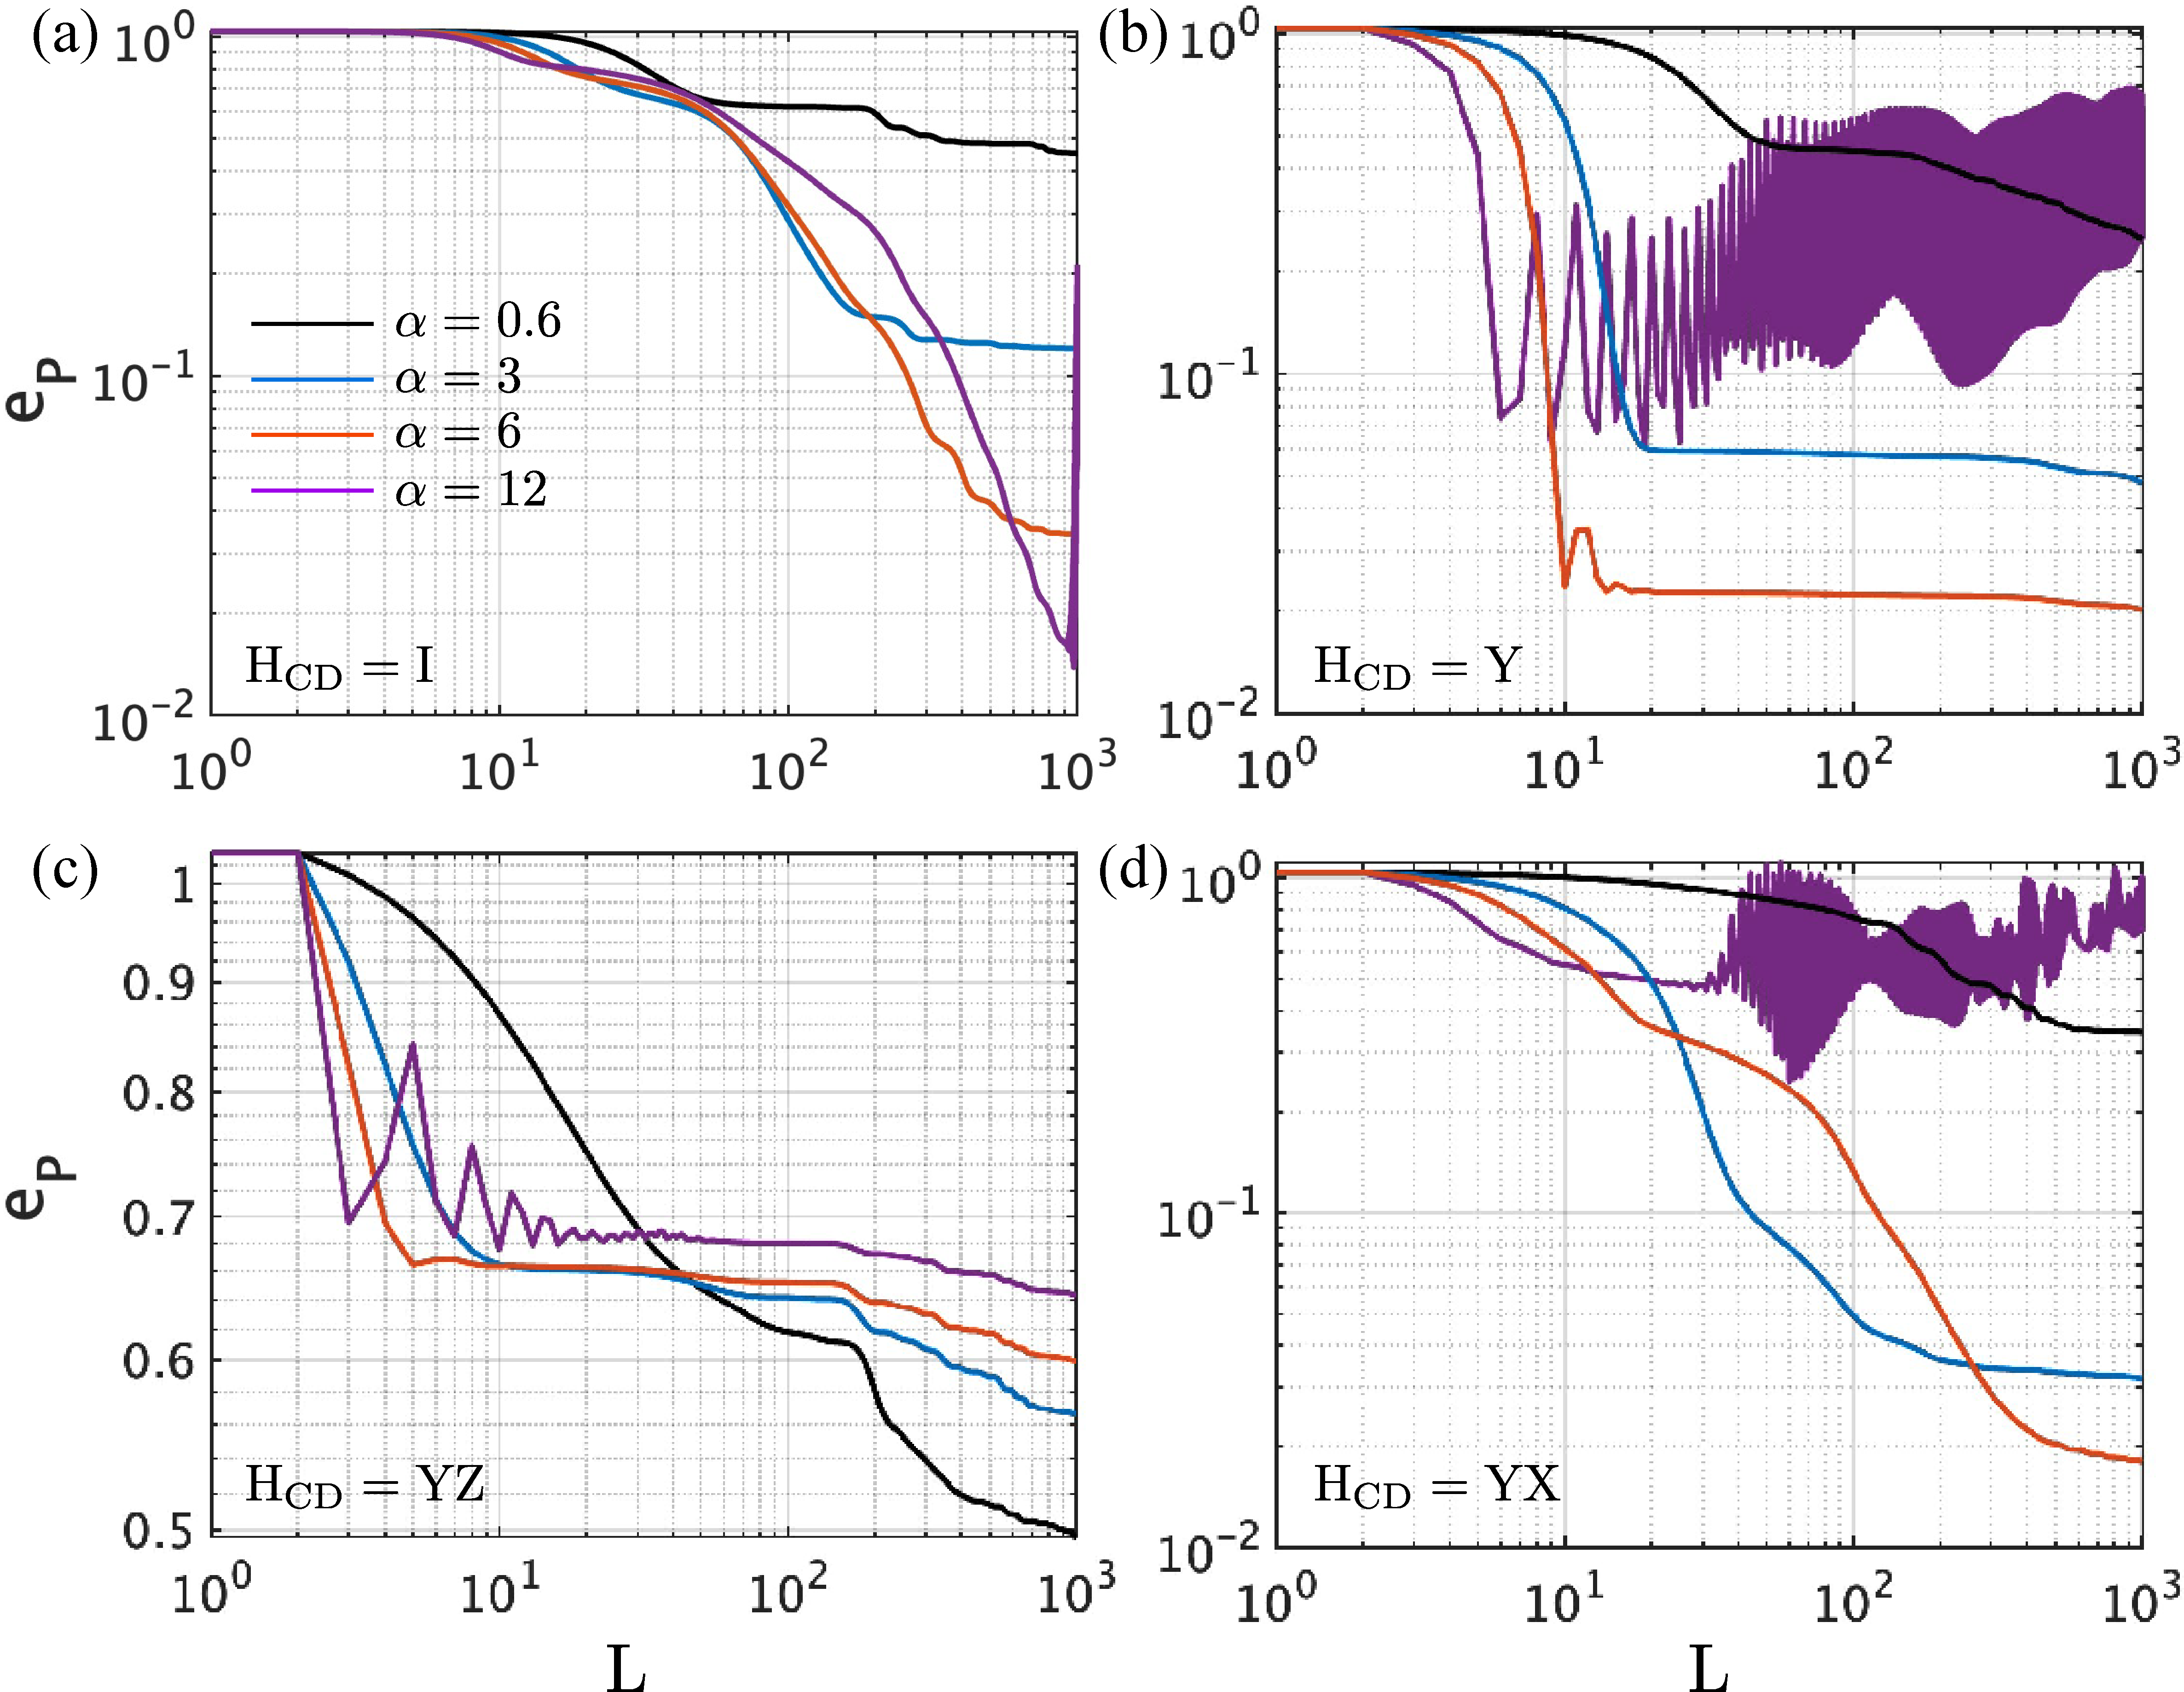
\includegraphics[scale=0.11]{alpha_final.pdf}
    \caption{Average energy difference per site shown as a function of circuit depth in log-scale for the MFI model
    for % different values of $\alpha$
    various $\alpha$ as specified in the legend
    in (a) for all panels, having $N=6$,
    $\Delta t = 0.01 / J$. % $\Delta t=0.01\,J$. // AW
    Each panel % plot
    corresponds to a different CD-FQA protocol
  % labeled by $H_{\rm CD}$ in the inset.
    for the $H_{\rm CD}$ as specified.
}\label{fig:alpha_final}
\end{figure}


\subsubsection{CD-FQA for different system sizes}
In Fig.~\ref{fig:N_final}, we present a comprehensive analysis of energy reduction versus circuit depth across a range of system sizes ($N=4$ to $N=10$) using various CD-FQA protocols, maintaining a fixed $\alpha=4$. The results depicted in all four figures underscore the \textit{robustness} of the CD-FQA protocol, demonstrating its independence from system sizes up to $100$ layers where $L\Delta t\sim 1$. Deviations in the curves for $N=4$ and $N=5$ are attributed to the influence of small system size. A noteworthy comparison can be drawn with the findings in Ref.~\cite{FeedbackPRL}, where the authors establish a linear relationship between the number of layers and system sizes. It is crucial to highlight a key distinction: unlike the approach in Ref.~\cite{FeedbackPRL}, our methodology involves normalizing the prefactor, as illustrated in \Eq{alpha}. Here, the parameters $\beta$ and $\gamma$ are normalized by a factor of $N$. 
For large circuit depth, % For a large number of layers, 
on the other hand,
we find across all panels in \Fig{N_final}
that the smaller system sizes show a somewhat
improved performance. This may be attributed
to the larger finite-size level spacing within
the excited states.
%the energy reduction for smaller system sizes
%outpaces that of larger system sizes. 
% This phenomenon is consistently observed across all four panels in Fig.~\ref{fig:N_final}, providing valuable insights into the efficiency dynamics of CD-FQA protocols with respect to circuit depth and system size.

The observed  
independence of the circuit depth for the above case is due the finite correlation length of the system
bearing in mind that the system is gapped. This 
has the advantage that
% non-trivial, yet highly desirable, as 
one can use the results of small sizes as an insight to design the protocol for large sizes.
%\awx{, for which numerical simulations are not possible. } 
Another relevant
comparison can be drawn with the findings in Ref. \cite{yao2021reinforcement}, where the authors, employing a
Reinforcement Learning method, observed similar independence of the number of layers on system sizes in a QAOA-type
architecture. In their study, unitaries composed of the MFI
Hamiltonian, $X$, and $Y$ were strategically ordered using a
policy derived from Reinforcement Learning techniques. The signature that the number of layers in a CD-FQA circuit is
nearly independent of the system size for the MFI model highlights the practical usage of such a protocol for large-system sizes. 








% As the system size increases, the slope of the curves
% becomes progressively steeper, indicating a more rapid rate of
% energy change, ultimately converging to the ground state energy
% within an error margin of $10^{-2}$. This observation results in
% a reduction in the number of layers required in the CD-FQA
% quantum circuit \aw{for larger systems. This suggests
% % Remarkably, for larger system sizes, these
% % curves are closely spaced indicating 
% an upper bound for the number of layers, and that the circuit depth}
% becomes independent of the system size for MFI % the MFI model
% in the CD-FQA protocol for the control field % when
% $Y$. %  serves as an additional control field. */==///


\begin{figure}
    \centering
    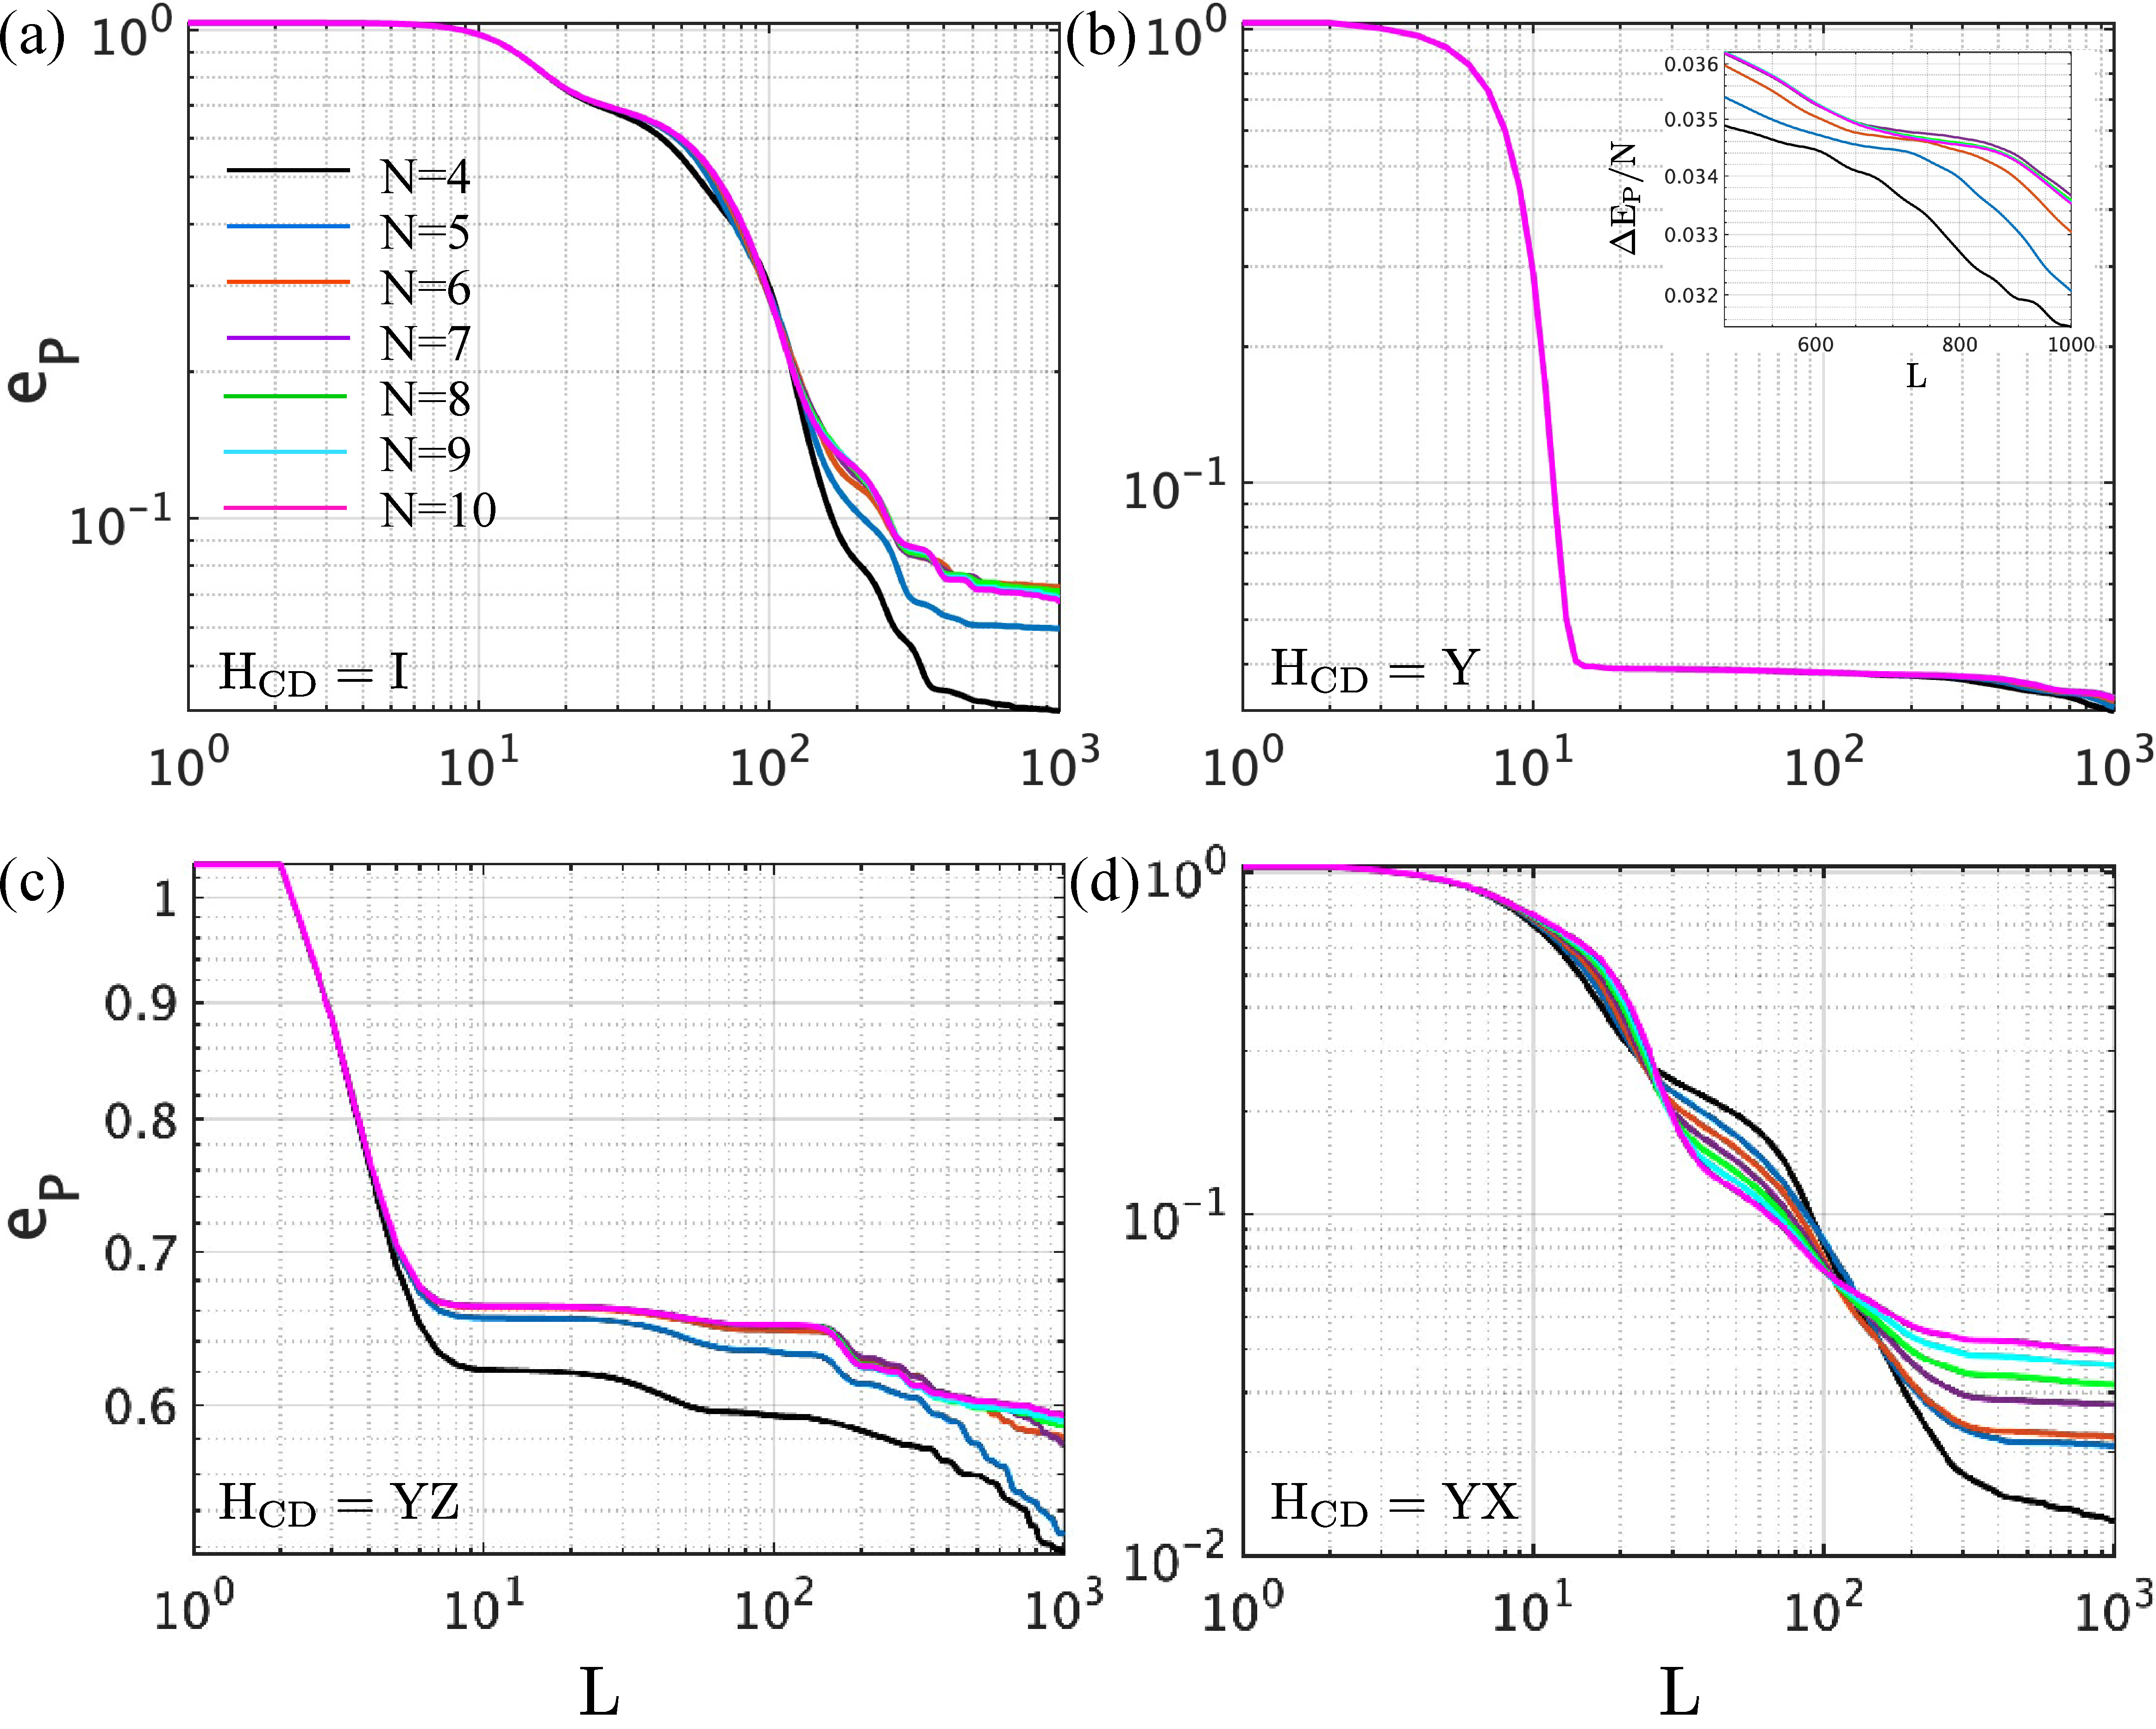
\includegraphics[scale=0.11]{N_final.pdf}
    \caption{Average energy difference shown as a function of circuit depth in log-scale for the MFI model
    for % different values of $N$
    various values of $N$ as specified in the
    legend in (a) for all panels,
    having $\alpha=4$, $\Delta t=0.01/J$. %  $\Delta t=0.01\,J$.
    Each panel % plot // AW
    corresponds to a different CD-FQA protocol
  % labeled by $H_{\rm CD}$ in the inset.
    for the $H_{\rm CD}$ as specified.
    The inset in (b) demonstrates the large-time behavior.
}\label{fig:N_final}
\end{figure}

\subsubsection{CD-FQA for different time-steps $\Delta t$}

Finally, % For completeness,
we also 
analyze the dependence % present the analysis
of the CD-FQA protocols on % for different values of
the value of $\Delta t$.
Larger % Smaller 
$\Delta t$ leads to a shallower % larger
circuit depth which is   
desirable % undesirable
for the implementation in a quantum circuit.
Too large a % Larger
$\Delta t$, however, can lead to a deviation from the QLC protocol that results in an energy increase
in \Eq{EP-dot}. In \Fig{deltat_final} we present the average energy decay as a function of 
the total simulated time
$T\equiv  L\Delta t$ for four values of $\Delta t$. For
$\Delta t \gtrsim 2\tau$,
% $\Delta t= 0.02 J$ and $\Delta t=0.03 J$,
and therefore $\alpha \Delta t \gtrsim 0.1/J$,
the CD-FQA protocol starts to oscillate after a few layers and the average energy does not decrease with circuit depth. 
The limit on $\Delta t$ to describe the differential
setting in \Eq{EP-dot} is thus comparable
to what one may use in a Trotterized setting,
bearing in mind that $\alpha$ enters as a scale
factor to the full Hamiltonian in \Eq{Schrodinger}.
Nevertheless, since we are not interested in the
the trajectory of the prepared state per se, but only
in the final result, in principle, this opens the
possibility to use adaptive $\Delta t$ along
the circuit starting from larger values.
We leave this additional fine-tuning as an
outlook for future studies.
For the present paper, however,
we keep $\Delta t$ constant throughout the circuit.

\begin{figure}
    \centering
    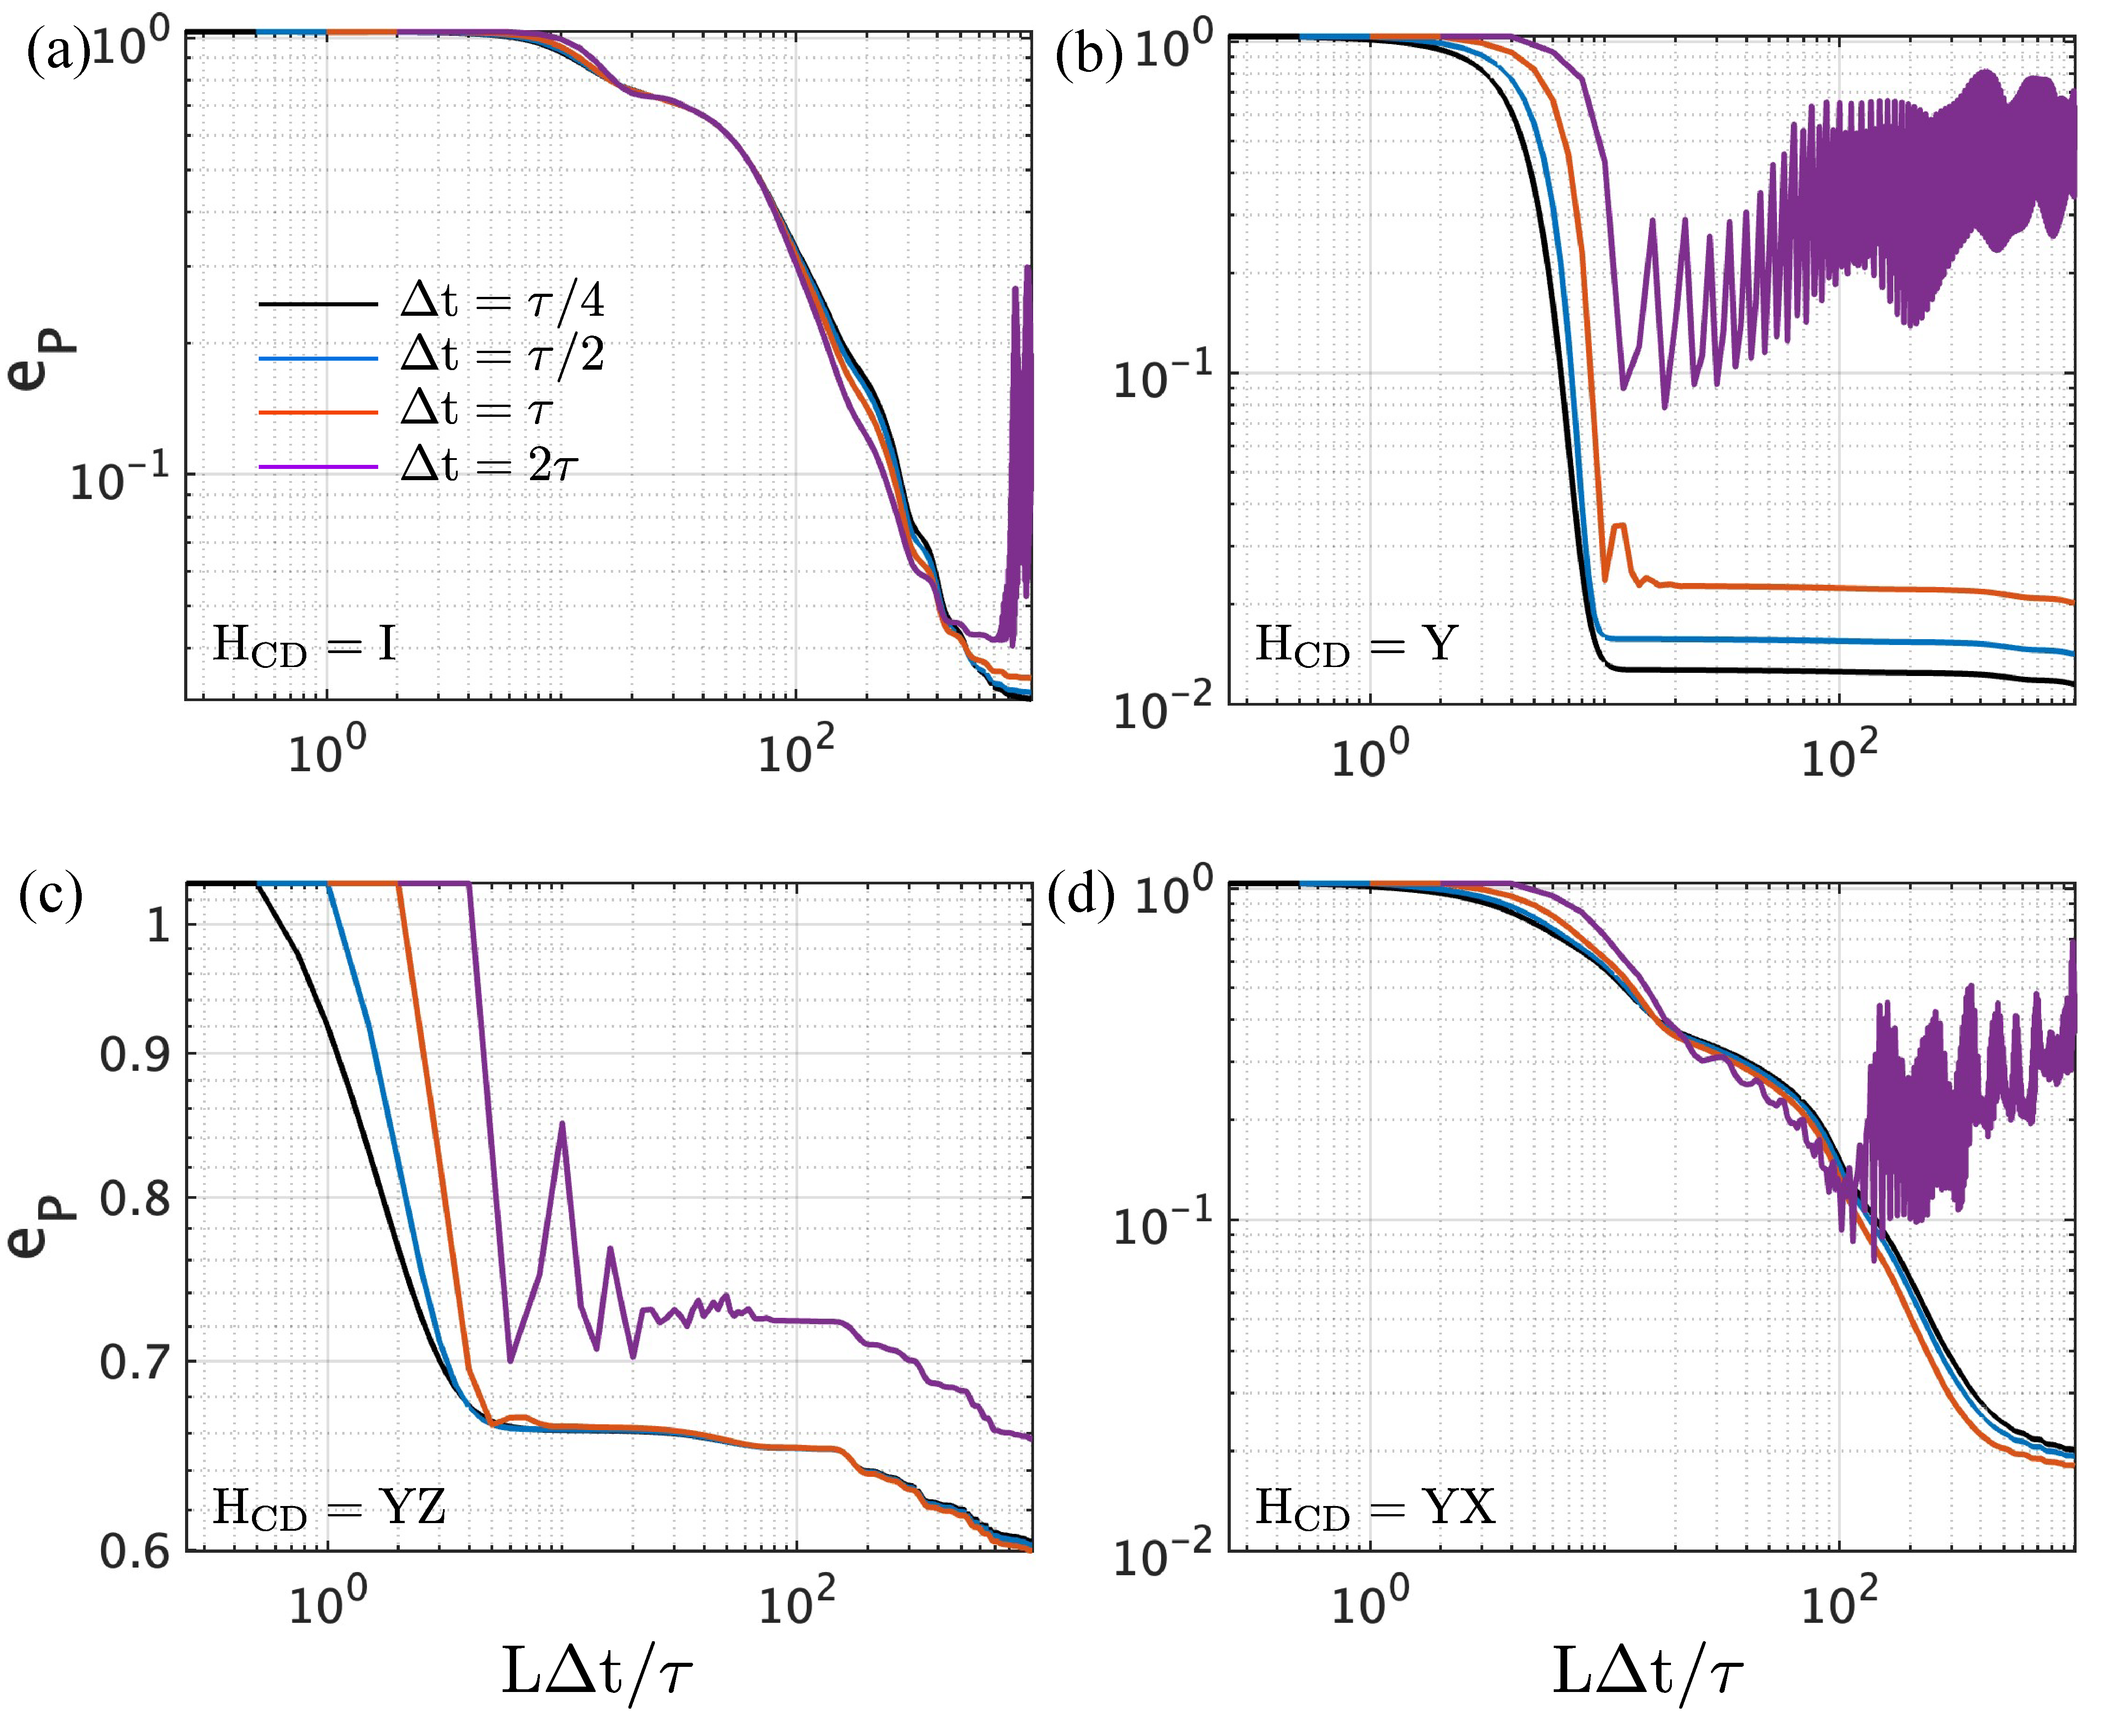
\includegraphics[scale=0.11]{deltat_final.pdf}
    \caption{
    %{\color{red}The y-axis labels on pancel c) above aren't correct, I think.} {\color{blue} This is in log-scale and YZ do not decrease the energy significantly.}
    Average energy difference shown as a function of circuit depth in log-scale for the MFI model
    for % different values of 
    various $\Delta t$ relative to the constant
    $\tau = 0.01/J$ % $\tau = 0.01\,J$ 
    used previously,
    with values specified in the legend of (a) for
    all panels, having $N=6$, and $\alpha=6$.
    Each panel % plot
    corresponds to a different CD-FQA protocol
  % labeled by $H_{\rm CD}$ in the inset.
    for the $H_{\rm CD}$ as specified.
  % labeled by $H_{\rm CD}$ in the inset.
    % Note that // AW
    Panel (c) demonstrates the early plateau behavior.
  % The system size is $N=6$, and $\alpha=6$.
  % \newline\awc{rather inlude $\tau/4$ instead of $3\tau$?}
  % \newline\awc{move blue and black lines to the foreground}
  % \newline\awc{in (c), why is the first blue data point at x=4
  % and not x=N=6? From the first data point, I'd think
  % that violett corresponds to $2\tau$?}
% AW: L=0 data point, i.e., "t=0" (initial value)
% is seen at -infty on log axis;
% first data point already should deviate from 
% initial value; currently it seems initial state is shown
% as first data point which suggests L=1, but is L=0 ?
}\label{fig:deltat_final}
\end{figure}
 
% In CD-FQA protocols with $H_{\rm CD}=Y$ and \YX, 
% by comparison [see \Fig{L1000} in \App{app:system-size}],
% % as we increase the system size, 
% the energies decrease at a faster rate initially
% when increasing system size.
% This slows down, however, at later times.
% followed by a slower rate at large times. These results are
% presented in \App{app:system-size}. % Appendix A.


\begin{figure}[tbh!]
\centering
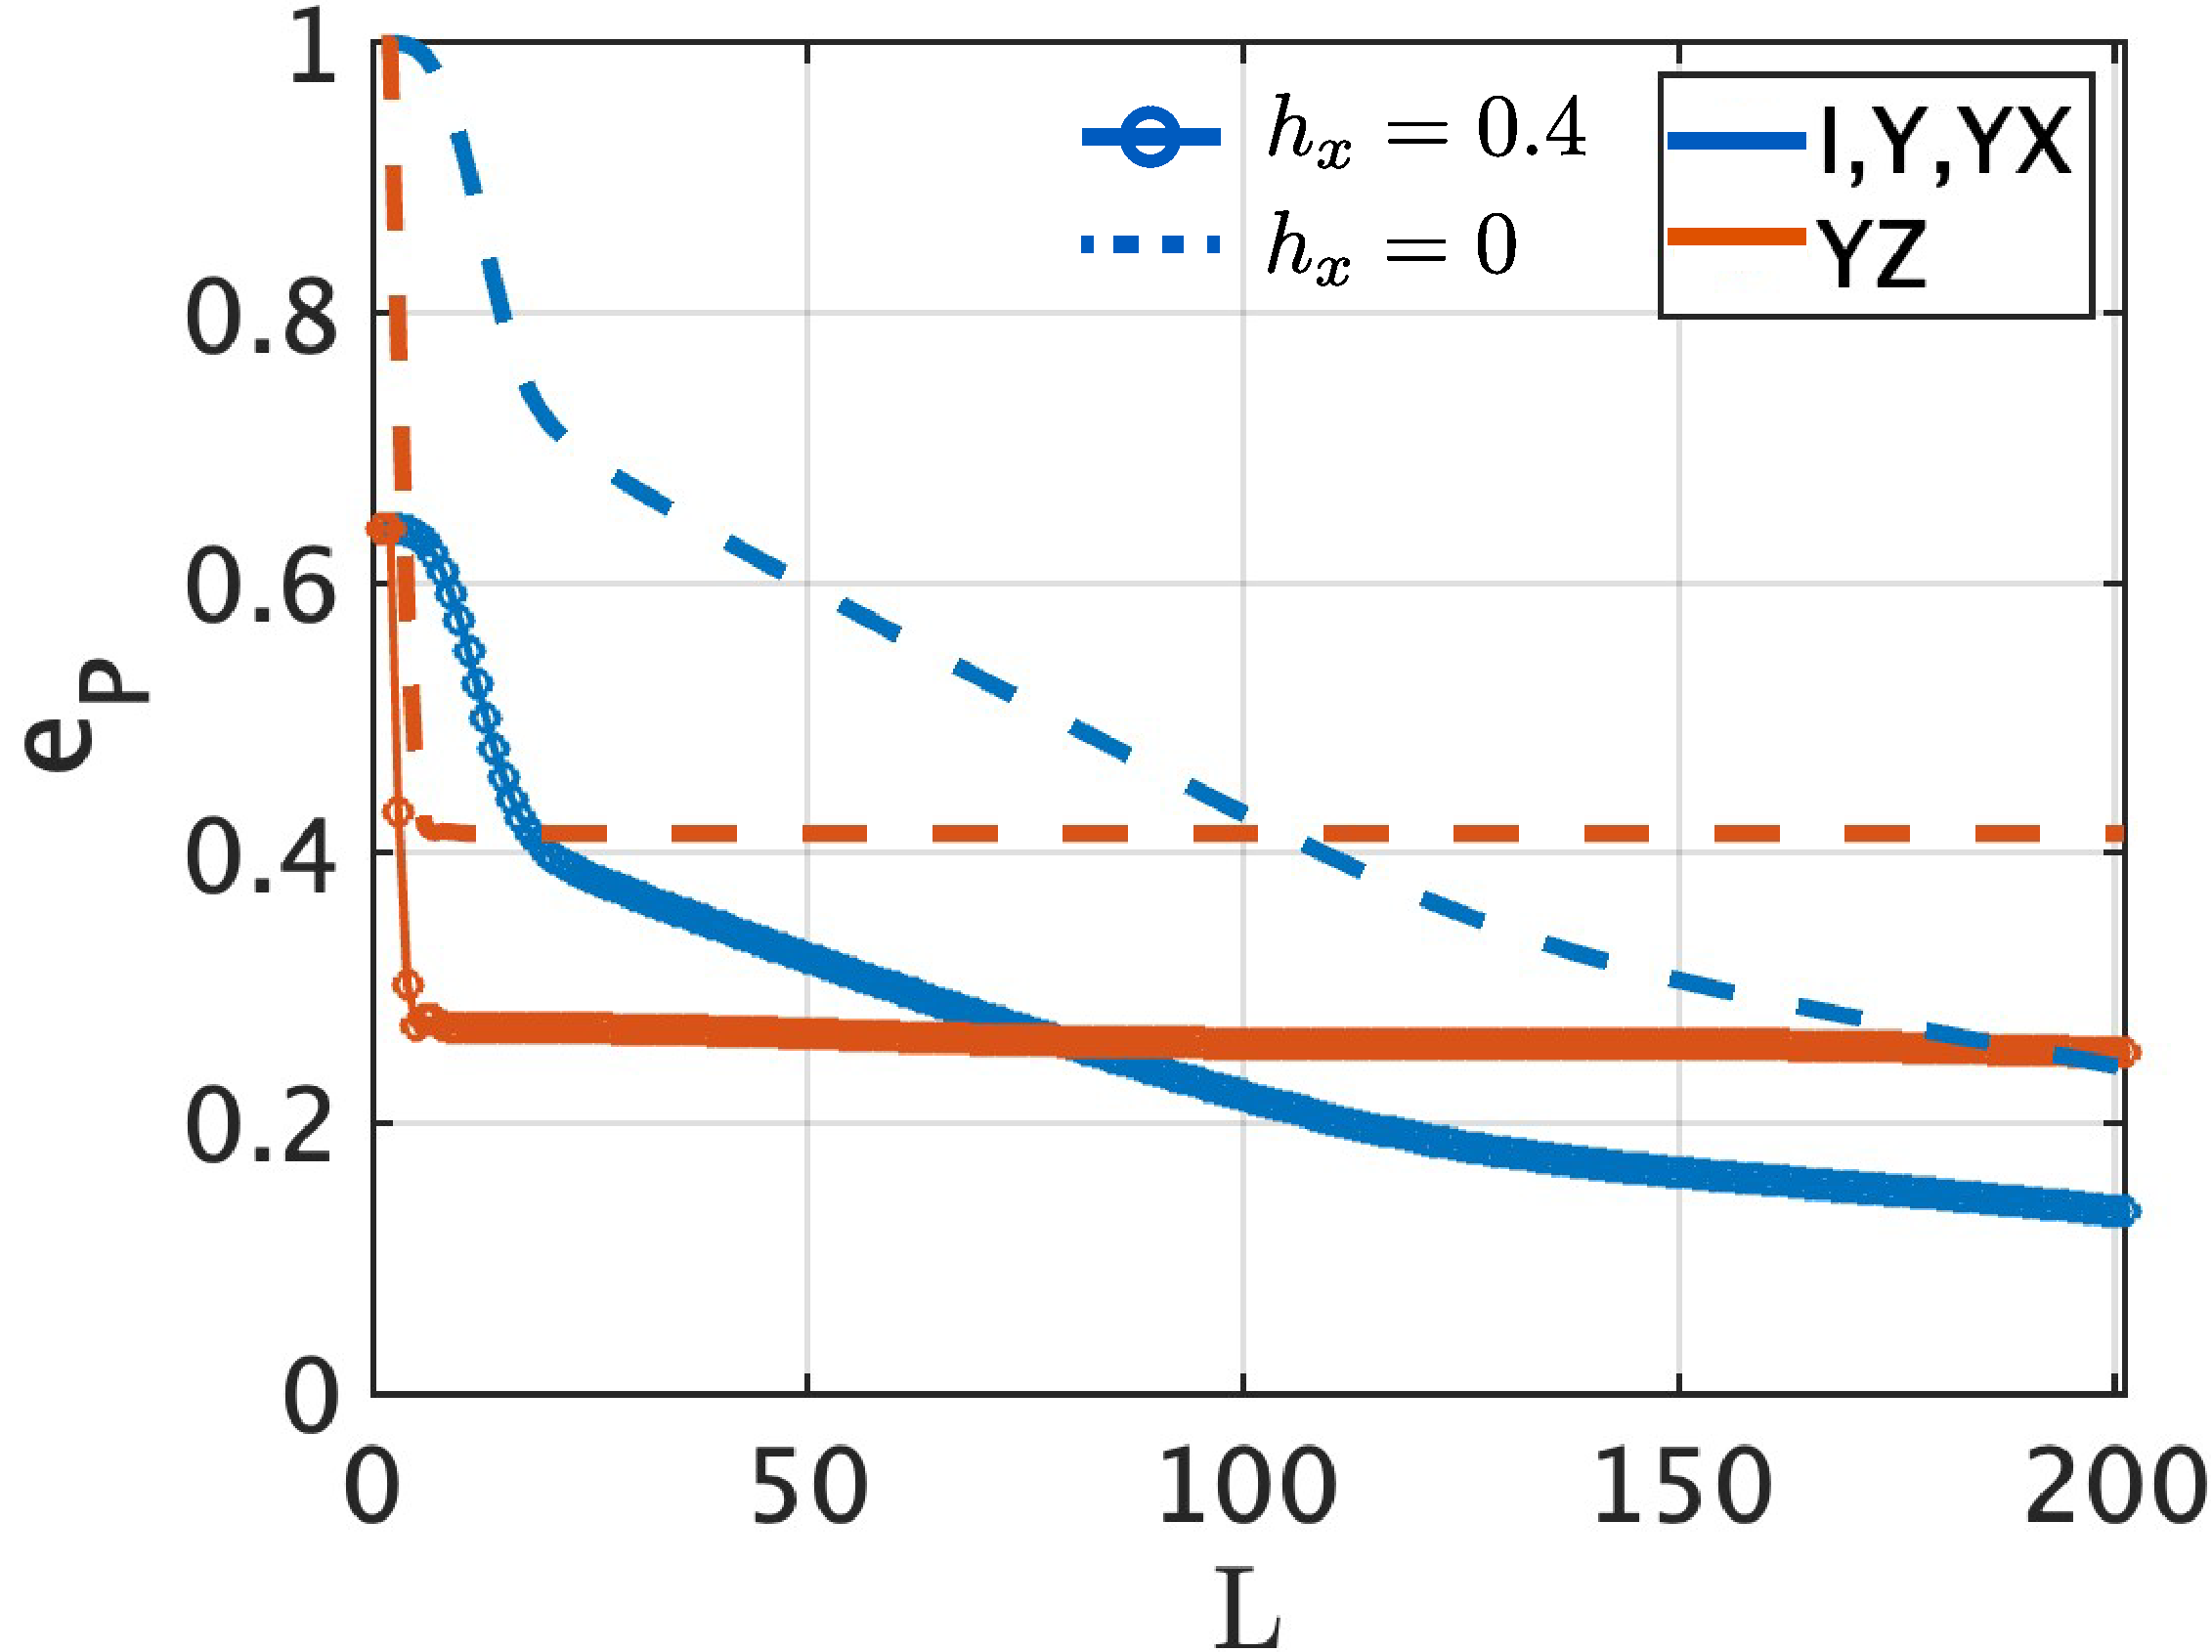
\includegraphics[scale=0.185]{TFIM.pdf}
% merged figures // AW
%\sidesubfloat[]{\label{:b}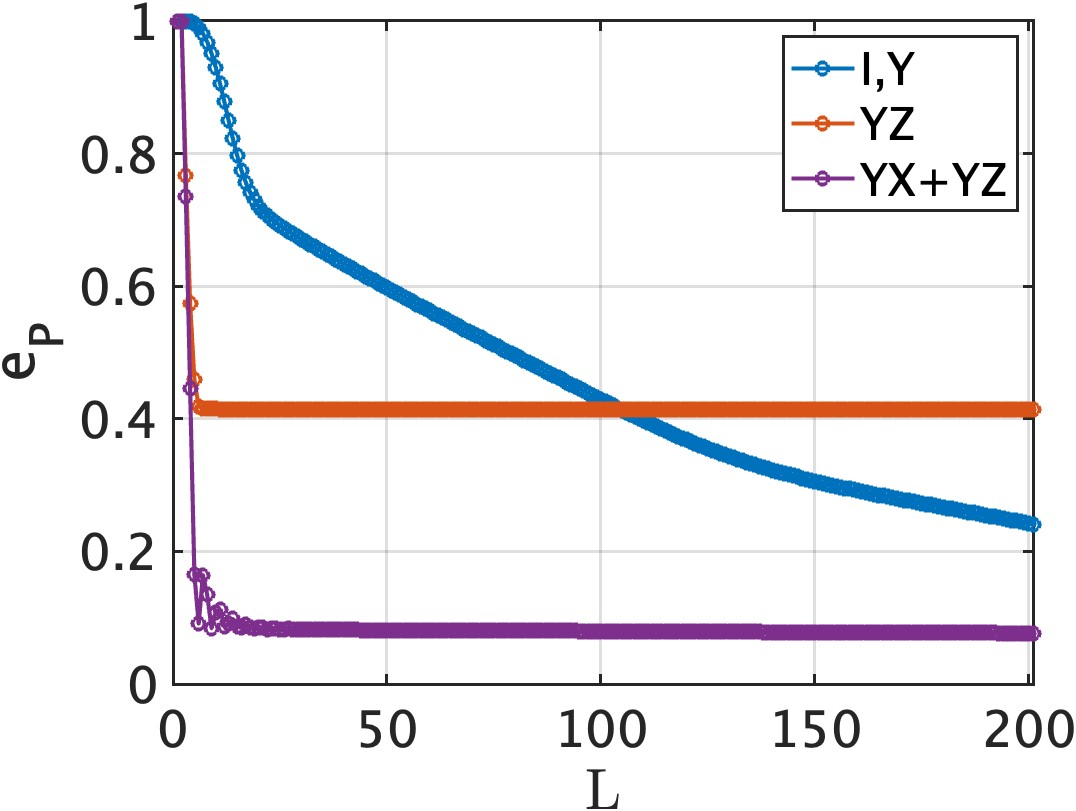
\includegraphics[scale=0.18]{special.jpg}}
\caption{
   Average energy % is shown as a function of the number of layers 
   vs. circuit depth for TFI with  $h_x=0.4$ (solid lines)
   and $h_x=0$ (dashed lines). The standard FQA and CD-FQA with $H_{\rm CD}=Y$ and $YX$ yield the same result. 
   %The purple curve represent $H_{\rm CD}=YZ+YX$, instead of $YX$ since the curve corresponding to $YX$ behaves similar to the standard FQA.
   %\awc{legend mismatch: there is no violet, but black?
  % make blue line black?}
}\label{fig:TFI}
\end{figure}
% AW: keep these figures together, as they belong together?

\begin{figure}
    \centering
    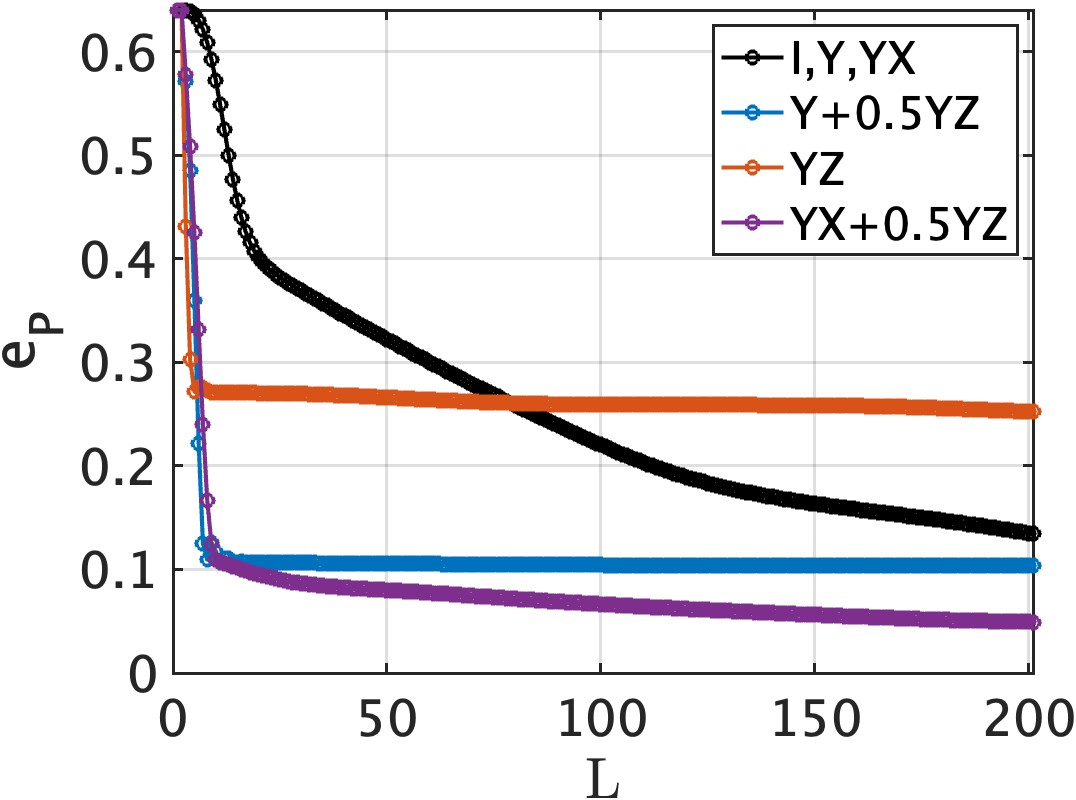
\includegraphics[scale=0.185]{Lcomb.jpg}
    \caption{Average energy
   vs. circuit depth for TFI with  $h_x=0.4$ with CD-FQA operator is a linear combination of two operators from the pool.
   }
    \label{fig:Lcomb}
\end{figure}



\begin{figure}[tbh!]
\centering
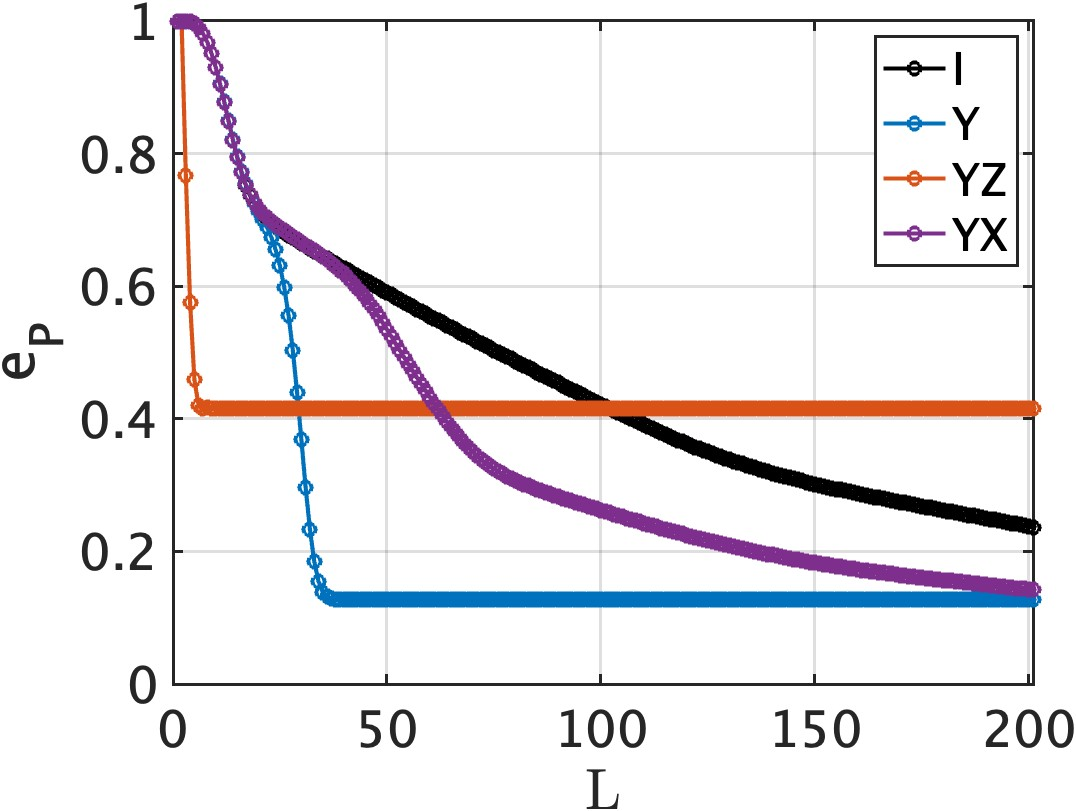
\includegraphics[scale=0.185]{GHZ100_pert.jpg}
\caption{ % The
   Average energy % is shown as a function of the number of layers
   vs. circuit depth for the TFI at $h_x=0$,
   % the special case where both $h_z$ and $h_x$ are zero
   but now including the  term
   $H_{\rm add}(k) % t
   =e^{-(k-1)/5} \, Z$ for layer $k$. % the $k^{\text{th}}$ layer.
   % \awc{match color coding with previous figure
   % where they agree?}
   % {\color{red}I'm not sure how the additional perturbative term is helping.  It looks like $H_{CD}=Y$ in Fig. 9 is no better than $H_{CD}=YX + YZ$ in Fig. 8b.}{\color{blue} This figure is an illustration that a small perturbation can accelerate a certain counterdiabatic protocol. YX+YZ demonstrates that a linear combination may be employed. Both are considered variations of standard CD-FQA protocol. I think I will add these arguments.}
}\label{fig:GHZpert}
\end{figure}


% AW: merged with above figure
% \begin{figure}
% \centering
% 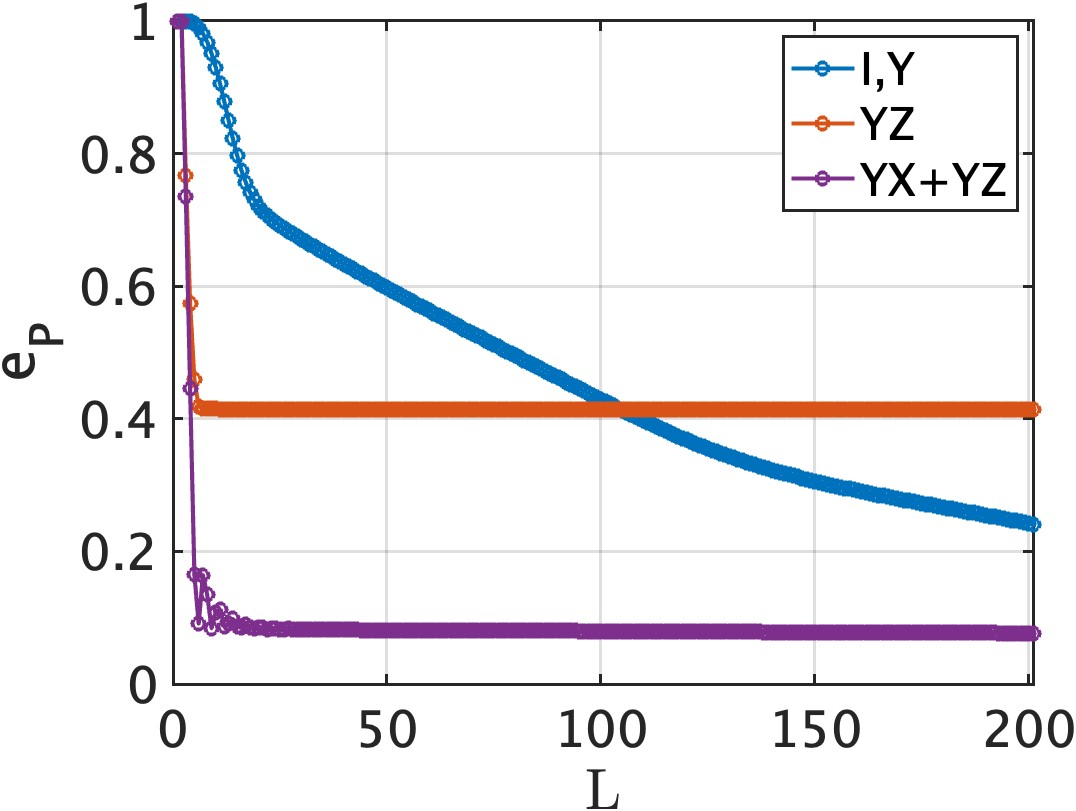
\includegraphics[scale=0.2]{special.jpg}
% \caption{
%    The average energy is shown as a function of the number of
%    layers for the special case $h_z=h_x=0$. % AW //  where both $h_z$ and $h_x$ are zero.
%    The standard FQA and CD-FQA with $H_{\rm CD}=Y$ yield the same result.
% }\label{fig:GHZ}
% \end{figure}

%%%%%%%%%%%%%%

% The TFI and the special case where $h_z=0$ and $h_x=0$
\subsection{TFI (including $h_x=0$)}
Now we apply the CD-FQA protocols to Ising chains with the longitudinal field turned off, i.e., $h_z=0$,
with the results presented in 
\Fig{TFI} for $h_x=0.4$, and  $h_x=0$.
% the CD-FQA protocol is
% presented for the TFI with ${ h_z, h_x}={0, 0.4}$ and the case
% where ${ h_z, h_x}={0, 0}$, respectively. 
The ground state of
the TFI is in the ferromagnetic phase and at $h_x=0$ there are
two degenerate ground states
$|\psi_{g1}\ra=|\uparrow\uparrow...\uparrow\ra$ and
$|\psi_{g2}\ra=|\downarrow\downarrow...\downarrow\ra$. 

The CD-FQA protocol employing the $H_{\rm CD}=\YZ$ operator
demonstrates a rapid energy reduction initially but becomes
exceedingly slow as we increase the number of layers, exhibiting
a plateau similar to the ones seen for LFI and MFI. This
protocol fails to reach the ground state, rendering it
undesirable. Notably, CD-FQA with $H_{\rm CD}=Y$ and \YX
mirrors the outcomes of the standard FQA, since $\gamma=0$ for all time steps.

In situations where the CD-FQA faces challenges in
convergence such as in \Fig{TFI} one may consider various approaches to improve the performance of the protocol. For instance, one may choose $H_{\rm CD}$ as a linear combination of operators from the pool of operators as the second control Hamiltonian, or add a small time-dependent Hamiltonian that vanishes at the end of the protocol.  


\subsubsection{Improving CD-FQA with linear combination of operators}

To address the limitations of the \YZ operator in the TFI model,
we first introduce the counterdiabatic operator as a linear
combination of two operators from the operator pool. In
\Fig{Lcomb}, we plot the CD-FQA protocol with $H_{\rm CD}=Y+
\frac{1}{2} % 0.5 // AW
\YZ$ and $\YX + \frac{1}{2} % 0.5 // AW
\YZ$ together with $H_{\rm CD}=\YZ$ and
the standard FQA.  The combination of these imaginary operators
promotes a better mixing between instantaneous eigenstates
compared to individual operators from the pool. As depicted in
\Fig{Lcomb} the CD-FQA protocol with linear combination achieves
a rapid decrease in average energy, surpassing the energy
obtained with the \YZ term alone. Although employing a linear
combination of multiple counterdiabatic operators circumvents
the plateau observed with a single counterdiabatic operator, the
implementation on a quantum circuit requires more than a single
layer. 

% The CD-FQA for the
% special case with $\{h_z,h_x\}=\{0,0\}$, yields similar results
% as the TFI. This similarity between the TFI and the special case
% mirrors the similarity between LFI and MFI.  Additional CD-FQA
% protocols for three other TFI models with parameters ${h_x}={
% -0.4}$, ${1.4}$, and ${-1.4}$, provided in Appendix A, exhibit
% similar behavior to Fig. \ref{fig:TFI}. 

\subsubsection{Improving CD-FQA with an additional time-dependent Hamiltonian}

Another viable strategy to improve the CD-FQA is to introduce a time-dependent term
into the dynamics. It is crucial to configure the time
dependence of the additional term in a manner such that the magnitude 
of the term gradually diminishes throughout the protocol,
ultimately reaching zero upon the protocol's completion.
Furthermore, the additional term must commute
with the problem Hamiltonian so that the protocol does not
introduce additional measurement for $\beta$ and $\gamma$.
%\hir{[The last sentence is not clear. Perturbation with $Z$ does affect $\beta$ and $\gamma$.]}

Let us illustrate this approach with a specific example,
considering the case where $H_P=-\ZZ$ and $H_1=X$. As previously
demonstrated, the counterdiabatic protocol with \YZ fails to
converge to the ground state, resulting in the average energy
plateauing at a value higher than the ground state. To address
this, 
% %{\color{red}I'm not sure how it addresses the poor performance of the choice $H_{CD}=YZ$?  It seems to be me still pretty poor. It does help  $H_{CD}=Y$ however.} {\color{blue} I agree. YZ is the worst. Y and YX give the same result as standard FQA. Therefore, 
% a perturbation helps us to improve Y and YX protocol. However, YZ still remains bad.}
we introduce a commuting time-dependent term,
denoted as $H_{\text{add}}=f(t_{k})Z$, where $t_k$ corresponds
to the time at the $k^{\text{th}}$ layer. The modified total
time-dependent Hamiltonian is now expressed as
$H(t)=H_{P}+H_{\text{add}}(t)+\beta(t)H_1+\gamma(t)H_{\rm CD}.$
The QLC protocol continues to be determined by the condition
$d\la H_P \ra/dt \leq 0$. However, the introduction of
$H_{\text{add}}(t)$ alters the effectiveness of counterdiabatic
operators, allowing the utilization of $Y$ as $H_{\rm CD}$ for
constructing the CD-FQA protocol. In Fig. \ref{fig:GHZpert}, we
present the average energy as a function of the number of
layers, incorporating the additional term and selecting
$H_{\rm CD}=Y$. The CD-FQA protocol with the additional term
exhibits better performance compared to the protocol with the
\YZ operator.

It is important to note that the introduction of the $Z$ term
breaks the degeneracy of the ground state of $H_{P}=-\ZZ$ as well as some of the excited states. 
Depending on the sign of the $Z$, the CD-FQA converges
to a state closer to one of the degenerate states within the
ground state manifold. Indeed, in our protocol, if it were not for the
$Z$, the state would be forced to flow to the GHZ
state, which is known to have a linear circuit
complexity~\cite{bravyi2006lieb, yu2023learning}, since both the initial state and the unitaries in CD-FQA are symmetric under $\prod_j X_j$.  

To see this, recall that we start with an initial state  $|{+}X\rangle$, and both $H_P$ and $H_1$ commute with $\prod_j X_j$. Operators from nested commutators (i.e., the \YZ operator) also commute with $\prod_j X_j$. Since we minimize the energy of $H_P=\ZZ$, when we are restricted to the $\prod_j X_j=1$ subspace, we are forced to flow to GHZ. An additional $Z$ term in the Hamiltonian biases the system towards either $|{+}Z\rangle$ or $|{-}Z\rangle$ and breaks away from the symmetry subspace. This addition of $Z$ further allows us to utilize $Y$ as a second control Hamiltonian. So one possible strategy to expedite conversion to a ground state is to select a
symmetry-breaking operator as the additional term when an obstruction due to long-range order is expected.


% Regarding what you mentioned, the $Y$ operator doesn't commute with $\prod_j X_j$, so it lifts the obstruction and the state can indeed flow to $|{+}Z\rangle$ or $|{-}Z\rangle$. The $Y$ operator results from the perturbation and helps go outside the symmetric subspace.]}
% %
% Introduction of the
% perturbation $Z$ breaks the symmetry $\prod_j X_j$ of the
% GHZ state and lets the state flow to one of the
% ferromagnetic states, which is reachable in a short-depth
% circuit. Therefore, one possible strategy to expedite
% conversion to a ground state is to select a
% symmetry-breaking operator as a perturbation when an
% obstruction due to a long-range order is expected.}
% %

Both strategies  employed above highlight the importance of alternate approaches to tweak the CD-FQA protocol to navigate
the quantum landscape effectively. However, one must take into
account that the introduction of an additional Hamiltonian
always increases the number of gates and thereby the depth of
the quantum circuit. 

Furthermore, in Appendix A, we extend our investigation for the TFI by exploring an alternative first control Hamiltonian, specifically $H_1=Z$, and the corresponding initial state $|\psi_0\ra=|\uparrow \uparrow ...\uparrow\ra$. The CD-FQA under this configuration exhibits superior performance compared to the scenario shown in Fig. \ref{fig:TFI}. All three counterdiabatic operators demonstrate better performance in achieving ground-state compared to the standard FQA Consequently, it is evident that the choice of $H_1$ significantly impacts the CD-FQA's performance in the context of the TFI. In this comparison, $Z$ emerges as a more favorable first control Hamiltonian than $X$ for the TFI, highlighting the importance of the specific control Hamiltonian selection in the CD-FQA.

\section{Demonstration on cloud quantum computers}
\label{sec:experiment}

% \begin{figure}
% \centering
% \includegraphics[width=1.0\textwidth]{FQAExperiments.png}
% \caption{
%    The average energy is shown as a function of the number of
%    layers for 4-qubit Ising model with Z perturbations performed
%    on ibm\_cairo. The parameters are $J=1$, $h_z=h_x=0$ and
%    $\Delta t = 0.02$. The dashed line indicates the exact ground
%    state energy.
% }
% \label{fig:experiment1}
% \end{figure}

\begin{figure}
\centering
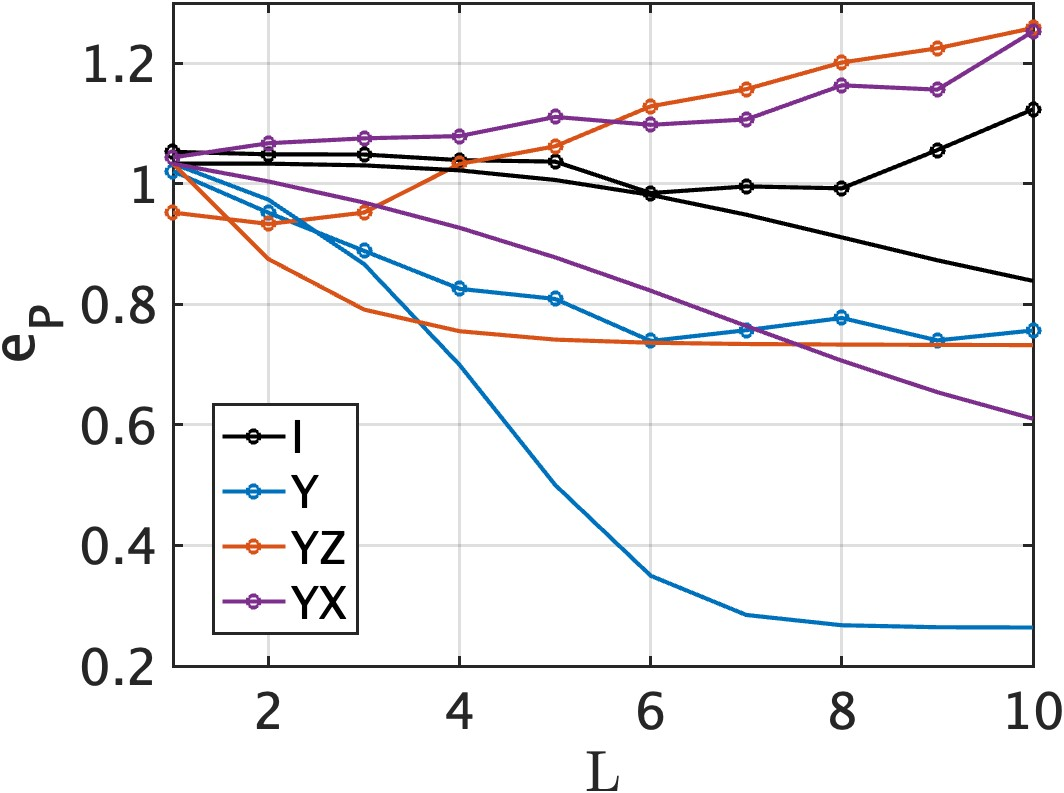
\includegraphics[scale=.2]{experiment.jpg}
\caption{
    The average energy is shown as a function of the number of
    layers for 4-qubit MFI with $h_z=h_x=0.4$ and $\Delta t = 0.02$.
    The simulation is performed on ibm\_hanoi with 8192
    repetitions for each measurement. The curves with markers
    represent data from quantum computers while the solid lines represent
    classical simulations.
}\label{fig:experiment}
\end{figure}


% \awc{describe what were the main bottlenecks here?
% likely obtaining $\beta$ and $\gamma$ was the most
% time consuming? was this obtained using an auxiliary qubit?}
%

To showcase the enhanced performance of CD-FQA over FQA on an
actual quantum platform, we conducted demonstrations
%; also see \url{https://journals.aps.org/pra/edannounce/cloud-quantum-computing-demonstrations-pra}. It is said ``We expect the layout of the computing device and its characteristics (qubit frequencies, qubit coherence times, couplings, gate and measurement fidelities, etc.) at the time of the demonstration to be presented in the paper. '']}
on IBM's
superconducting quantum computer through cloud-based
simulations. Employing CD-FQA for the MFI with a four-spin system with OBC, for parameters $h_x=h_z=0.4$. The outcomes,
illustrated in Fig. \ref{fig:experiment}, reveal a consistent
monotonic decay of energy in FQA and Y-FQA up to the
$6^{\text{th}}$ layer. Conversely, in the \YZ case, we observed a
decrease only up to the $2^{\text{nd}}$ layer, and \YX failed to
exhibit any decay even in the first layer.

Considering the impact of gate noise inherent in quantum
circuits, deploying a substantial number of 2-qubit gates
 resulted in undesirable outcomes. Therefore, in conventional FQA 
% {\color{red}Conventional FQA corresponds to $I$, correct? From Fig. 10 it doesn't look so good.  I would say instead the CD-FQA with Y outperforms all other choices.} {\color{blue} Okay}.
and CD-FQA utilizing the Y operator, where local operators are
employed as $H_1$ and $H_{\rm CD}$, we found such circuits demonstrated a decrease in energy performance up to the $6^{\text{th}}$ layer. Moreover, the CD-FQA with $Y$ performs the best.
The state generated after the application of numerous layers
exhibited an undesirable growth in energy, a phenomenon
unsuitable for any protocols. The influence of noise became
evident in measurements, where all Pauli operator expectation
values approached zero. Nevertheless, for a limited number of
layers, we observed an enhancement of CD-FQA over conventional
FQA in terms of both energy accuracy and convergence speed,
particularly in the case of Y-FQA.


% For the special case $h_x=h_z=0$, we added a decaying
% perturbation term $\sum_i Z_i$ to break the symmetry of the
% original Hamiltonian, which leads to much faster convergence.



% is
% shown in Fig.~\ref{fig:experiment1} and \ref{fig:experiment}.

\section{Discussion}
\label{sec:discussion}

% {\it (i)} Originally counterdiabatic driving was introduced to
% correct nonadiabatic transitions. Unlike the original idea,
% here, we exploit the interplay between the QLC and the
% counterdiabatic driving protocol to accelerate the
% feedback-based quantum algorithm for the ground state
% preparation of a many-body quantum system.  In the QLC
% protocol, the system starts with a superposition of many
% eigenstates of the problem Hamiltonian. If the system follows
% the adiabatic path then it would end up with a superposition
% state. So, finding an exact gauge potential to make the system
% adiabatic for the QLC  is rather counterproductive.  Instead,
% we only use the counterdiabatic operators to build a control
% Hamiltonian that can facilitate the mixing between
% eigenstates. Together with the constraint imposed on the
% Lyapunov function counterdiabatic operator enhances the
% population transfer to the desired state.   

An important aspect of 
CD-FQA lies in the strategic selection of the
additional % second
control Hamiltonian, % denoted as 
$H_{\rm CD}$,
within the given context of the provided $H_P$ and $H_1$.
This choice significantly influences the evolution of the control
field $\gamma(t)\propto \la [H_P,H_{\rm CD}] \ra$  % AW: removed |...|
which depends on % a quantity linked to 
both, the commutator and the state $\psi(t)$. % under consideration.
In our investigation with $H_1=X$,
the initial state is chosen as the ground state
of $-H_1$, % $H_1=X$, represented as 
$|\psi_{0}\rangle = |X\rangle \equiv |\rightarrow\rightarrow \ldots \rightarrow\rangle $.
As this extremizes $\la X \ra$,
a strategy to enhance the energy
reduction via $\gamma \sim \langle [H_P, H_{\rm CD}] \rangle$
at early times is to look for operators $H_{\rm CD}$ that yield
$ [H_P, H_{\rm CD}] \sim X$. Given our initial state, 
therefore the commutators resulting in $X$ or \XX lead
to the largest $\gamma$'s at early times. This leaves only
a few choices for $H_{\rm CD}$:
\begin{subequations}\label{eq:HCD:dominant}  \\
\begin{eqnarray}
   H_{\rm CD} &=& Y                   \label{eq:HCD:Y}  \\
   H_{\rm CD} &=& \YX \text{ or } \XY \label{eq:HCD:YX} \\
   H_{\rm CD} &=& \YZ \text{ or } \ZY \label{eq:HCD:YZ}
\end{eqnarray}
\end{subequations}
since for \Eq{eq:HCD:Y}, $[(H_P \to Z),Y] \sim X$, 
for \Eq{eq:HCD:YX}, e.g., $[(H_P \to Z), \YX] \sim -\XX + \YY$.
For these to occur, this also shows the importance of the
longitudinal term $Z$ in $H_P$ to be present. 
The last option in \Eq{eq:HCD:YZ} arises since, e.g., 
$[(H_P \to \ZZ), \YZ] \sim - \mathit{XZZ} - \mathit{ZXZ}$
where the diagonal terms in \ZZ lead to $X$.
In all cases, $H_{\rm CD}$ needs to include $Y$.
This makes intuitive sense, since $Y$ is required to rotate
the initial state $|X\rangle$ to $|Z\rangle$ which is close
to the Ising ground state, exactly so for $h_x=0$.


% Therefore when the commutator $[H_P,H_{\rm CD}]$
% closely aligns with the $X$ operator, the initial values of
% $|\gamma(t)|$ reach their maximum. For the four cases considered
% in our study, the set of possible commutators includes
%    $[Z,Y]\propto X$, 
%    $[\ZZ,Y]\propto \XZ+\ZX$, 
%    $[Z,\YZ] \propto \XZ$,
%    $[\ZZ,\YZ] \propto X + ZXZ$, 
%    $[Z,\YX] \propto \XX+\YY$, and
%    $[\ZZ,\YX] \propto \XY + \XY$. 
% Given our chosen initial state, only the
% commutators involving $X$ or \XX survive in the beginning. 

In the presence of the $Z$ term in the Hamiltonian
(LFI and MFI) % scenarios of LFI and MFI, 
% the commutators involving $Y$
% and \YZ generate $X$, while the commutator with \YX yields
% \XX. Consequently, 
all three counterdiabatic operators in \Eqs{eq:HCD:dominant}
exhibit a rapid reduction in average energy values over a small
number of layers.
% This behavior is clearly seen in the corresponding figures. 
As seen in \Figs{LFI} and \ref{fig:MFI},
the best performance for long times is given by $a>b>c$
% (Y > YX) > YZ
[based on the subequation numbering in \eqref{eq:HCD:dominant}].
Notably, the one with the worst long-term performance ($c$) 
%{\color{red}isn't $c$ meant?}{\color{blue} Yes}
demonstrates the fastest energy reduction at early times.
% YZ > (Y > YX)
This shows that focusing solely on the most rapid energy reduction in the choice of $H_{CD}$
can drive the system into barren plateaus in terms of quasi-steady
states at elevated energy [cf. \Fig{MFIcolor}c].
% \awc{actually would expect $\YX \to \XX$ being
% fastest at early times, because $\langle \XX \rangle
% \gg \langle X \rangle $ for the initial state $|X\rangle$;
% why \YZ?}\raj{RM: I think $\langle \XX \rangle = \langle X \rangle $, since the number of terms are same and all the spins are aligned along x.}


In stark contrast, in % for the TFI and the special case,
the absence of the $Z$ term in the Hamiltonian (TFI,
 including $h_x=0$), only the option in \Eq{eq:HCD:YZ} remains in order to effectively reduce the energy, as also seen in \Fig{TFI}. 
 %{\color{red}I don't understand.  From \Fig{TFI} it is YZ+ZX that is best -- which is not even an option in Eqn. 17.} {\color{blue} I agree. The eq. 17 basically includes one layer gates. But a linear combination will require more than one layer to implement. However, I think we should make some comments on YZ+ZX. }
% $(YZ+YX) > YZ > (Y=I)$
In this case, using \Eq{eq:HCD:Y} has no effect
whatsoever, with the data identical to plain FQA.
Similar to the LFI case, however, the \YZ operator
is prone to getting stuck at finite energy.
As seen in \Fig{TFI},
adding \YX, while irrelevant at early times,
nevertheless does permit to drive the system to
lower energy after the initial stage. 


We have also addressed variations of the CD-FQA protocol to overcome the early plateaus seen in \Fig{TFI}. The two approaches involve incorporating a linear combination of two operators from (\ref{eq:HCD:dominant}) or adding a time-dependent term to the $H_{P}$ that diminishes over time. Such variations yield excellent results for the TFI.

% AW: commented out remainder
% renders the
% commutators with $Y$ and \YX incapable of generating $X$, and
% \XX terms, respectively. Therefore, the CD-FQA with \YZ yields
% a different curve than the standard FQA.  The subtle interplay
% between the choice of control Hamiltonian and the specific
% characteristics of the Hamiltonian terms contributes to the
% effectiveness and adaptability of the CD-FQA across diverse
% quantum systems.

 Feedback-based quantum algorithms require a deep circuit with many layers and are beyond the scope of the current NISQ devices. However, a shallow FQA circuit can be utilized to ``warm start" a QAOA-type quantum circuit, i.e., to use the FQA parameters $\beta_{k}$ to initialize the QAOA algorithm. Note that, each layer in QAOA is parametrized by two real numbers, and one of the parameter is $1$ and the second parameter is approximated by $\beta_{k}$. 
 We observe that a similar extension is also possible for the CD-FQA, where one can utilize the parameters of CD-FQA circuit to warm start a VQA, where each layer is parameterized by three layers. This translates to a digitalized-counterdiabtic inspired QAOA \cite{chandarana2022digitized} where the initial parameters are selected from the CD-FQA.    

\section{Conclusion}
\label{sec:conclusion}

In this study, we have extended the FQA by incorporating the
principles of QLC  with the counterdiabatic driving protocol.
Departing from the conventional use of a single control field,
we propose the integration of a second control field inspired by
the counterdiabatic driving protocol. This modification proves
instrumental in accelerating ground state preparation,
showcasing its effectiveness for implementation on digital
quantum circuits. The CD-FQA has been systematically applied to
four distinct variants of the Ising models. Our results showcase
the intricate interplay between various parameters involved in
the CD-FQA and how a proper selection of the second control
Hamiltonian depends on the problem Hamiltonian, first control
Hamiltonian, and the initial state for fast preparation of the
ground state. On the one hand, % Furthermore, 
the introduction of a second
control field contributes to an increase in complexity within a
single layer. On the other hand, this % while 
effectively reduces the overall circuit complexity.  
These two system-dependent aspects need to be
balanced for optimal performance.
% As an application, we highlight that 
The parameters of the presented FQA can serve
as an initial seed for further classical optimization.
% Inspired by these findings, we emphasize the
This opens the
potential for extending the CD-FQA parameters to set up QAOA
circuits, thus allowing one to combine % bridging the gap between 
quantum and classical
optimization methodologies. This is particularly noteworthy, as
previous research has successfully demonstrated a three-unitary
QAOA utilizing a similar operator pool
\cite{chandarana2022digitized}. Beyond its applications in
quantum optimization algorithms, the CD-FQA unveils novel
possibilities in the realm of fast quantum control methods
employing counterdiabatic driving protocols. This convergence of
quantum algorithmic advancements and control theory holds
promise for shaping the future landscape of quantum computing.
In conclusion, our work not only enhances the understanding of
ground state preparation in quantum many-body systems but also
adds insights for quantum control strategies with far-reaching
implications in the field.

\section{Acknowledgments}

The authors thank Ning Bao and Ananda Roy for useful discussions. All authors of this work were supported in its production by the U.S. Department of Energy, Office of Basic Energy Sciences, under Contract No. DE-SC0012704.
%\raj{\bf{[Please add the funding info...]}}  \textcolor{blue}{[For SBU part, we don't need to acknowledge any other federal grants, only to acknowledge an internal fund. All of us can be attributed to DOE and we don't need to explicitly write RKM, AW and RMK...; instead: This work was supported by the U.S. Department of Energy,...]} 
TCW acknowledges the support of an SBU Presidential Innovation and Excellence (PIE)
Fund.

\appendix
% \begin{figure}[h!]
% \centering
% 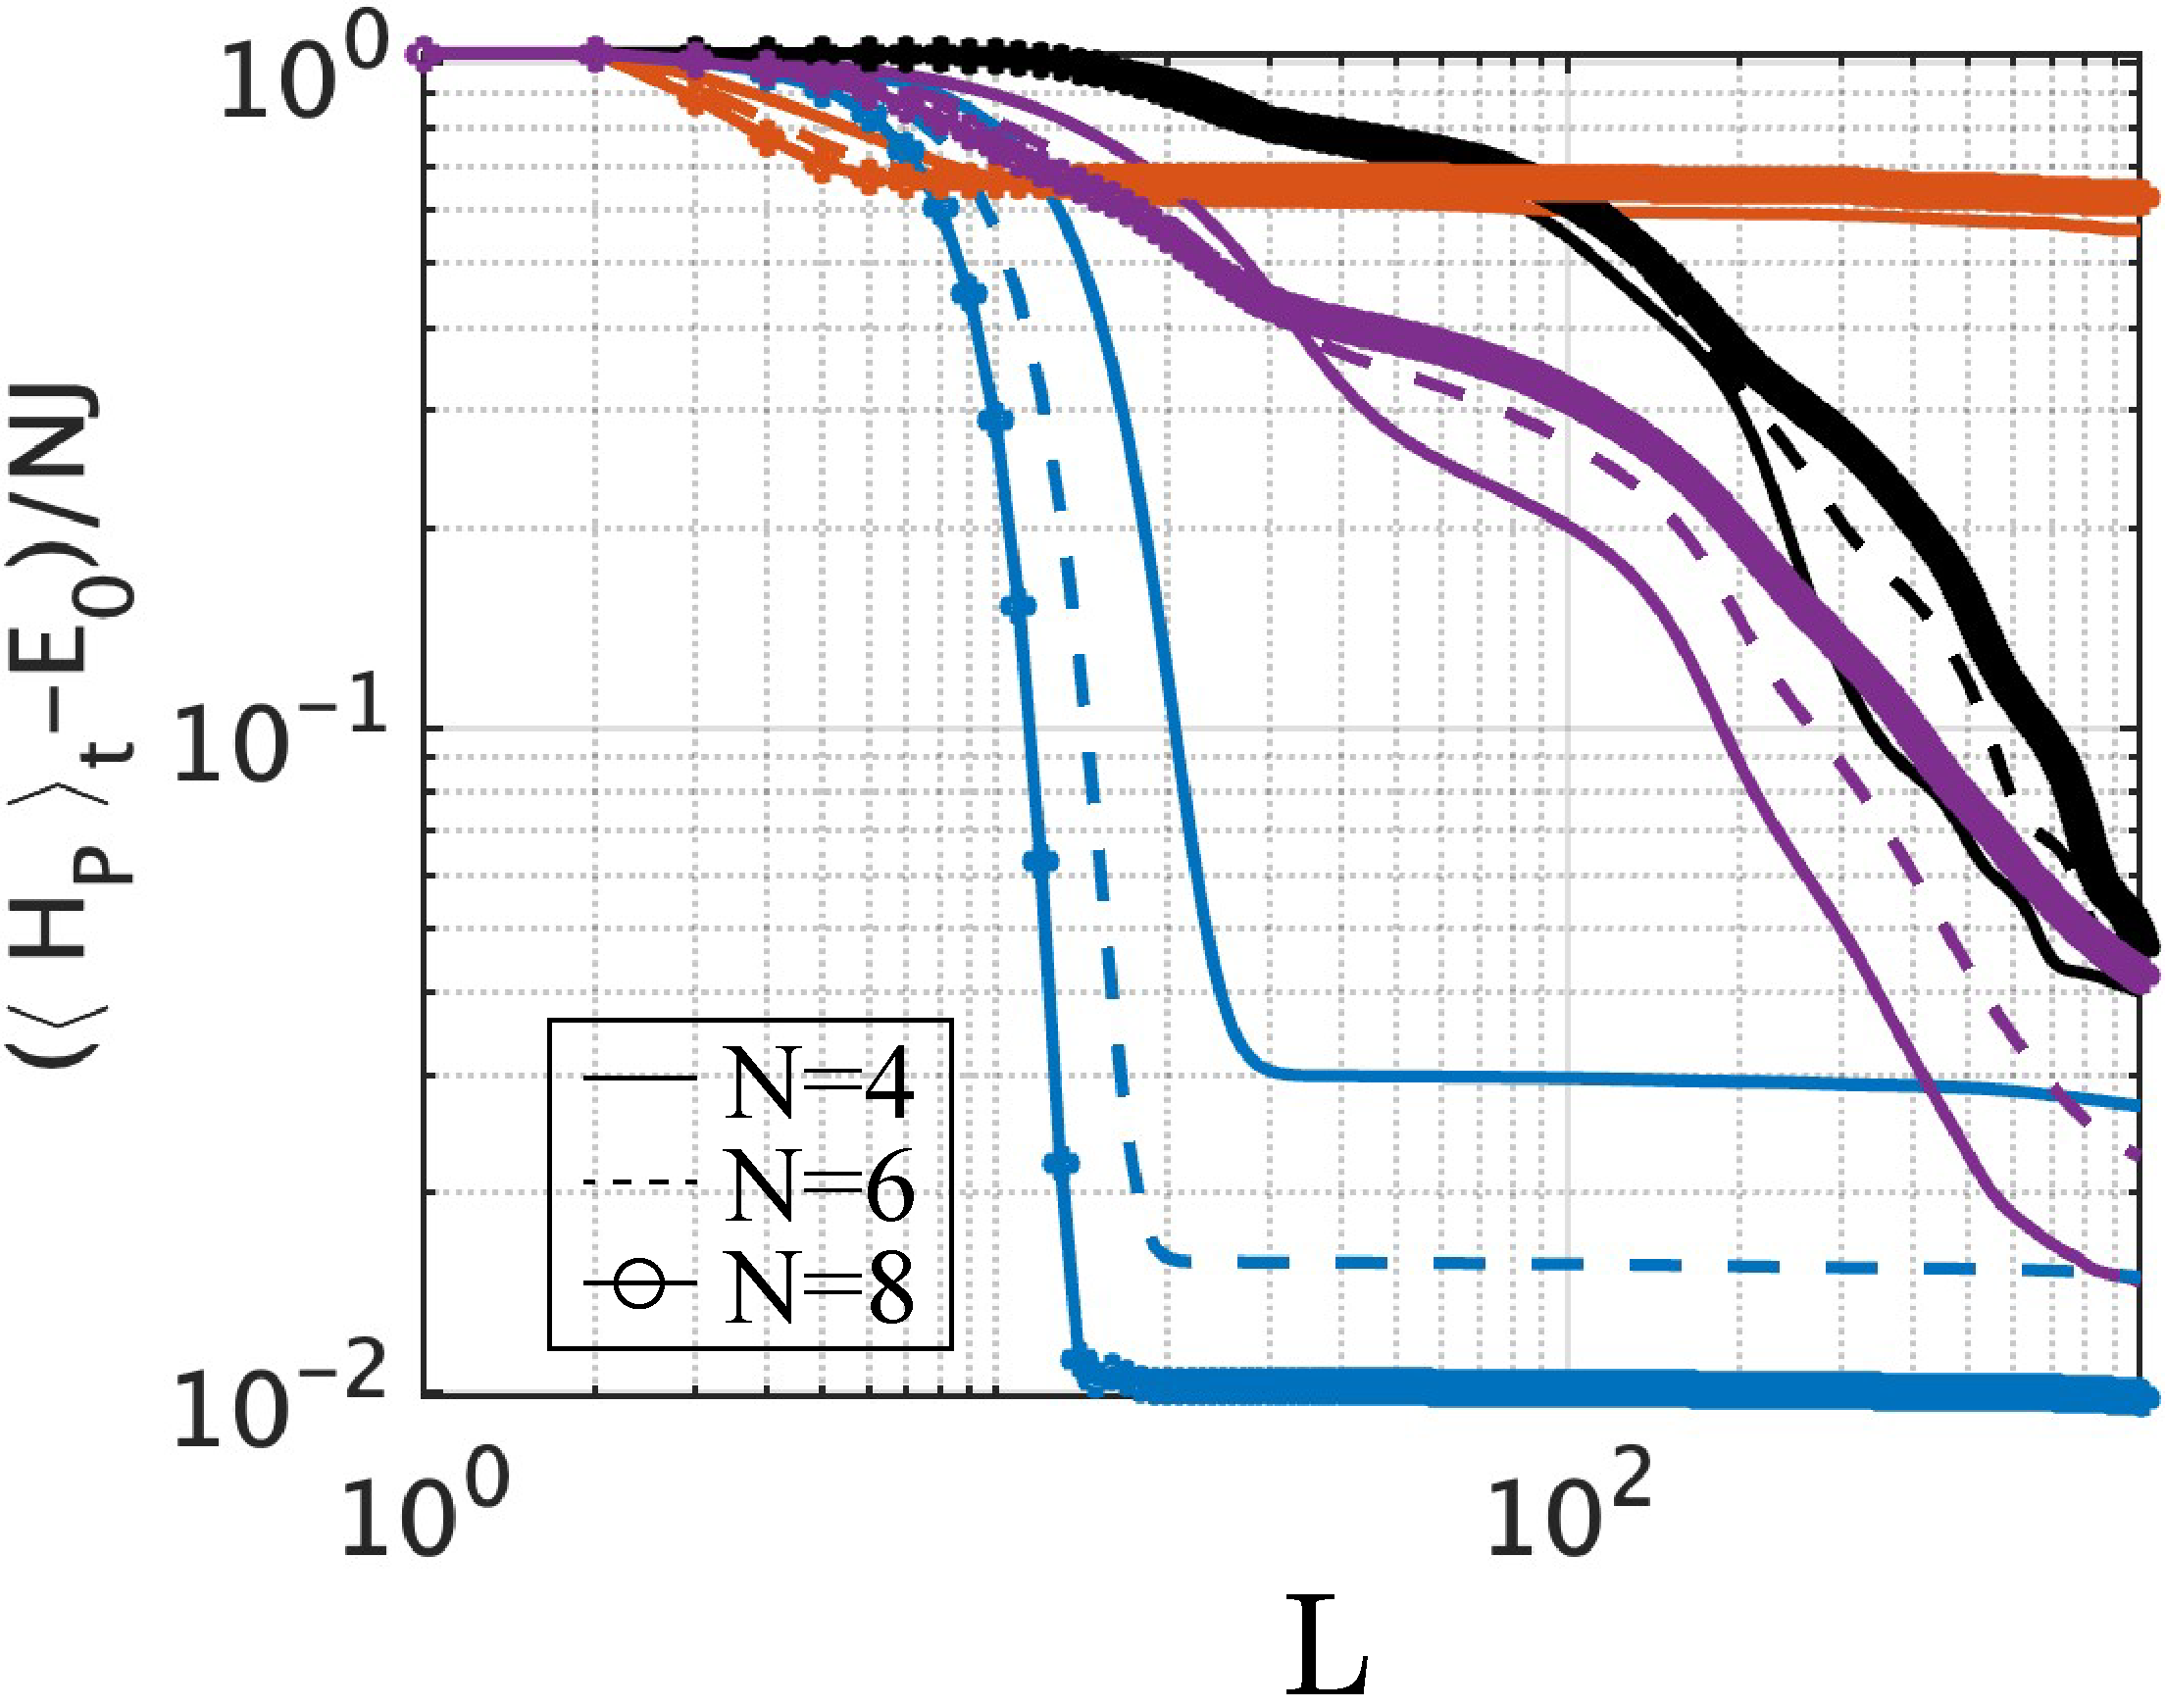
\includegraphics[scale=0.2] {MFIMA1.pdf}
% \caption{
% (a) The average energy in the CD-FQA protocol 
%   % up to % for 
%   % 1000 layers 
%     is shown for the MFI \aw{using the parameters
%     as in \Fig{MFI}, yet for various system sizes % with
%     $N=4,6,8$.} \awc{move legend to panel (a); 
%     also repeat legend from \Fig{MFI}; align panels}
% (b) \aw{Same as panel (a) but for significantly extended
%     circuit depth and plotted on log-log scale}.
%   % The average energy in the CD-FQA protocol for MFI is shown
%   % for different system sizes in log scale. For clarity, we
%   % have used $\Delta t=0.005$. All other parameters are same
%   % as Fig. \ref{fig:MFI}.
% }\label{fig:L1000}
% \end{figure}

\begin{figure}[h!]
    \centering
    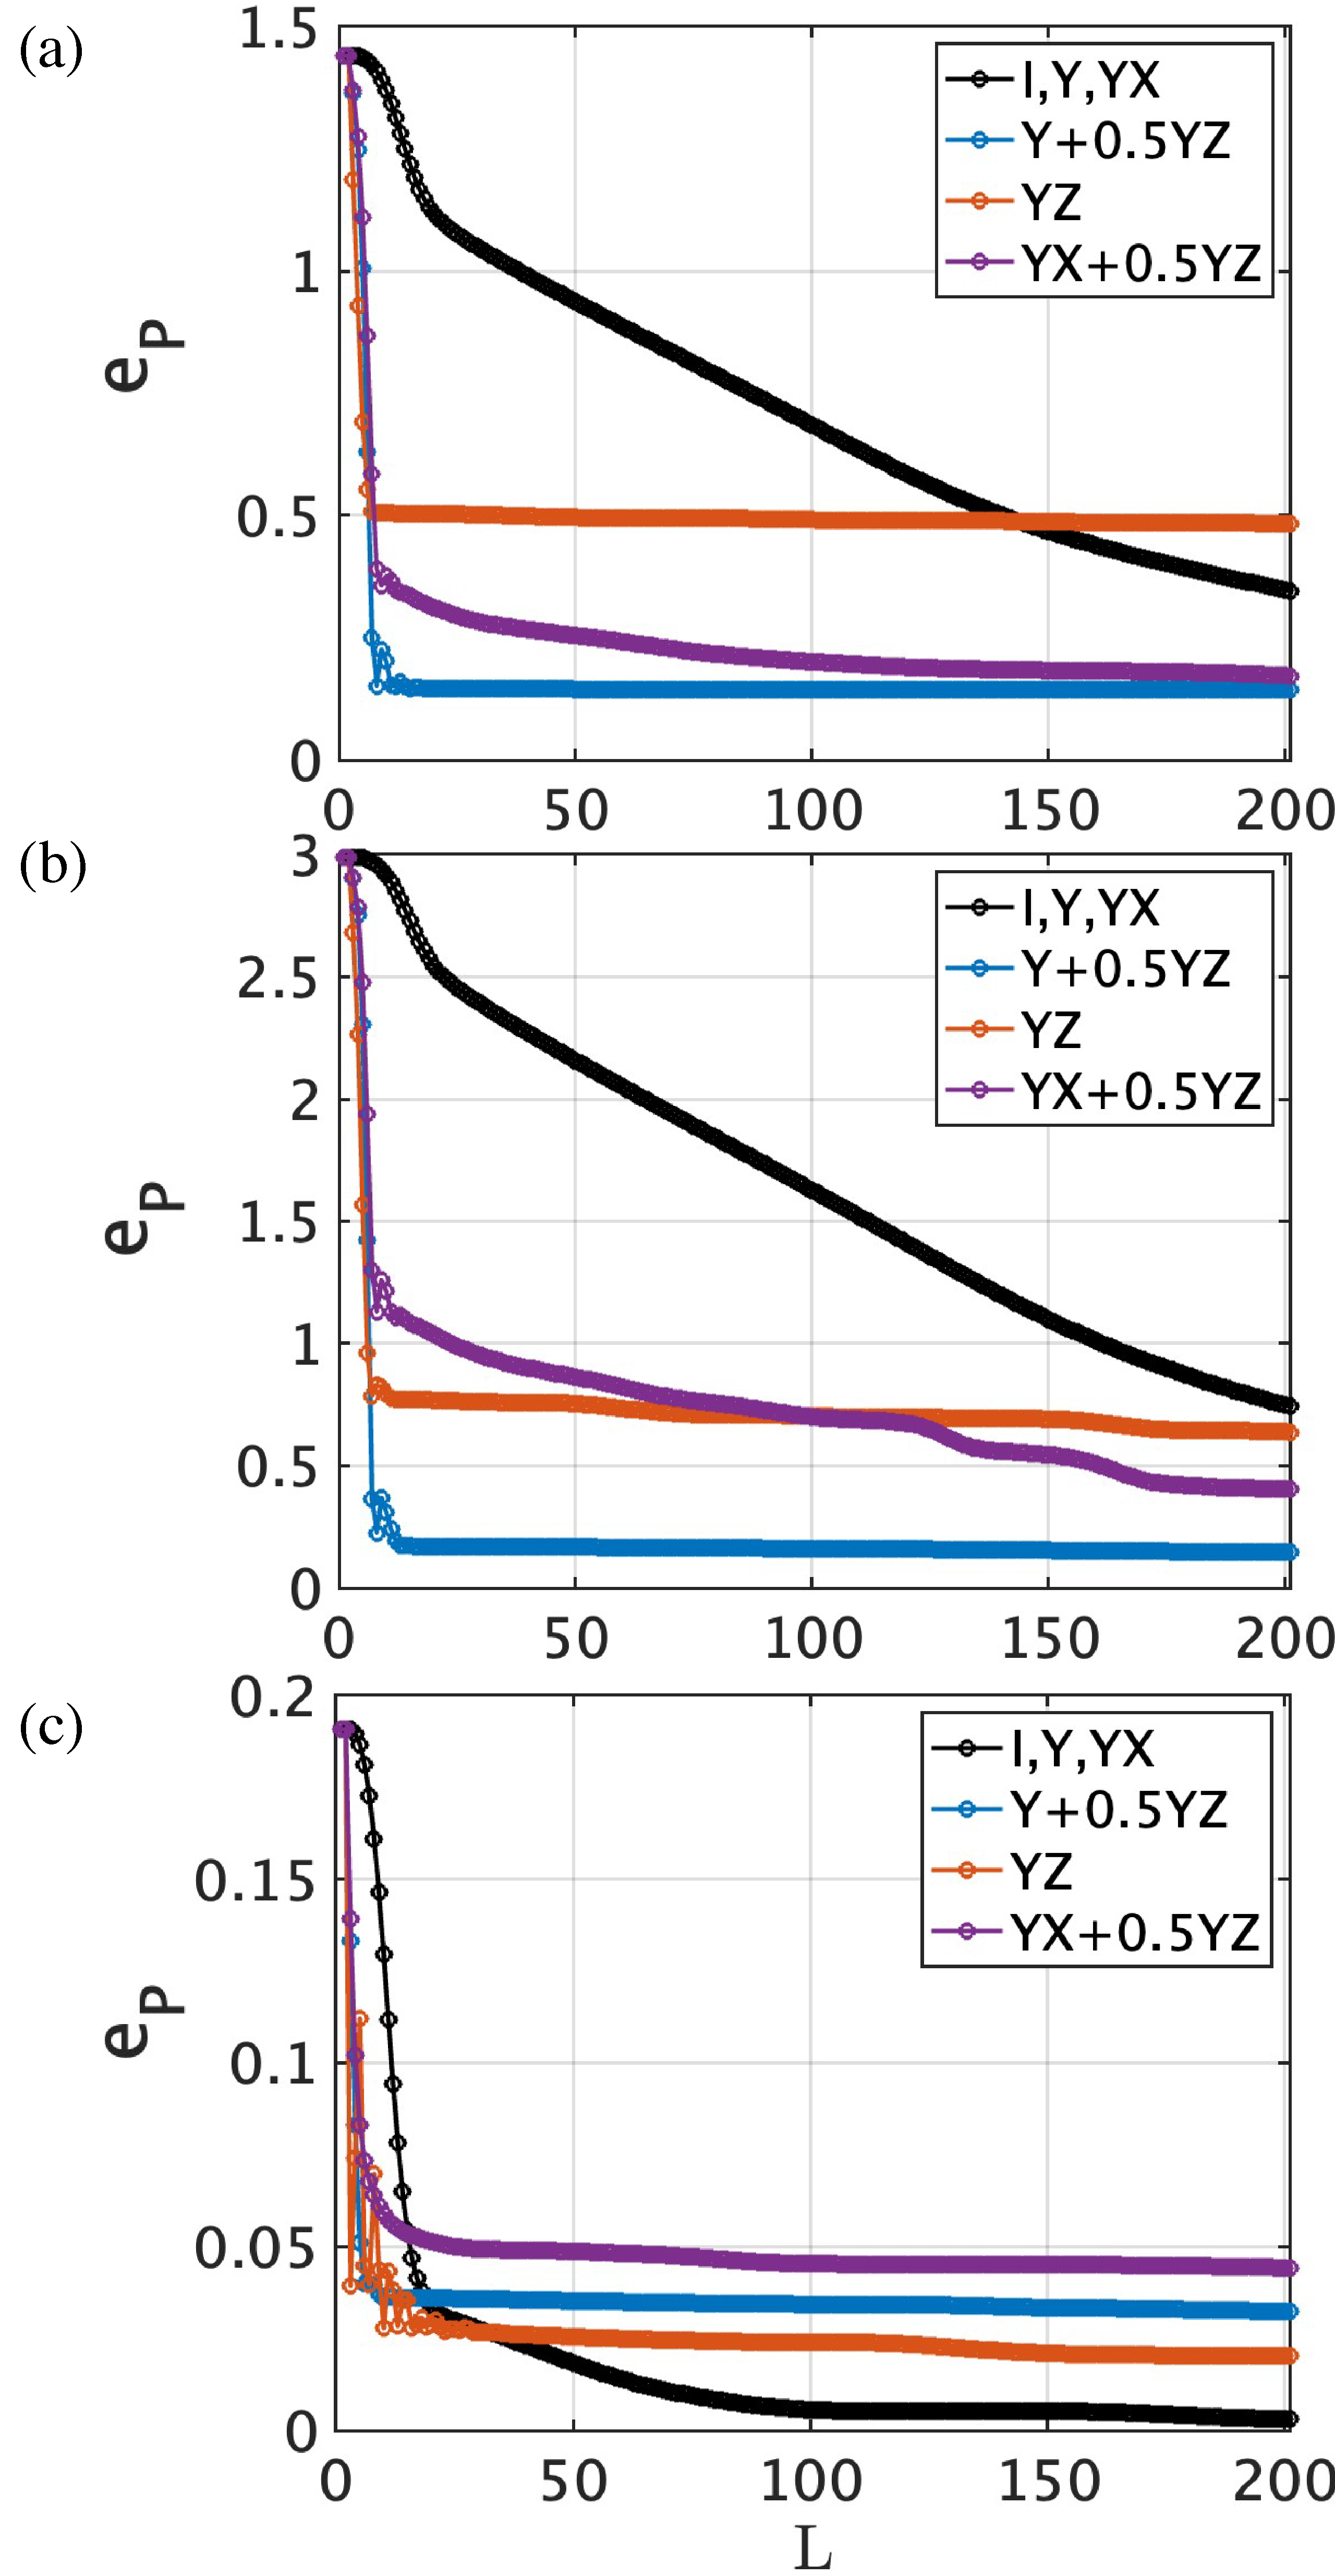
\includegraphics[scale=0.2]{TFIadd.pdf}
    % \sidesubfloat[]{\label{:a}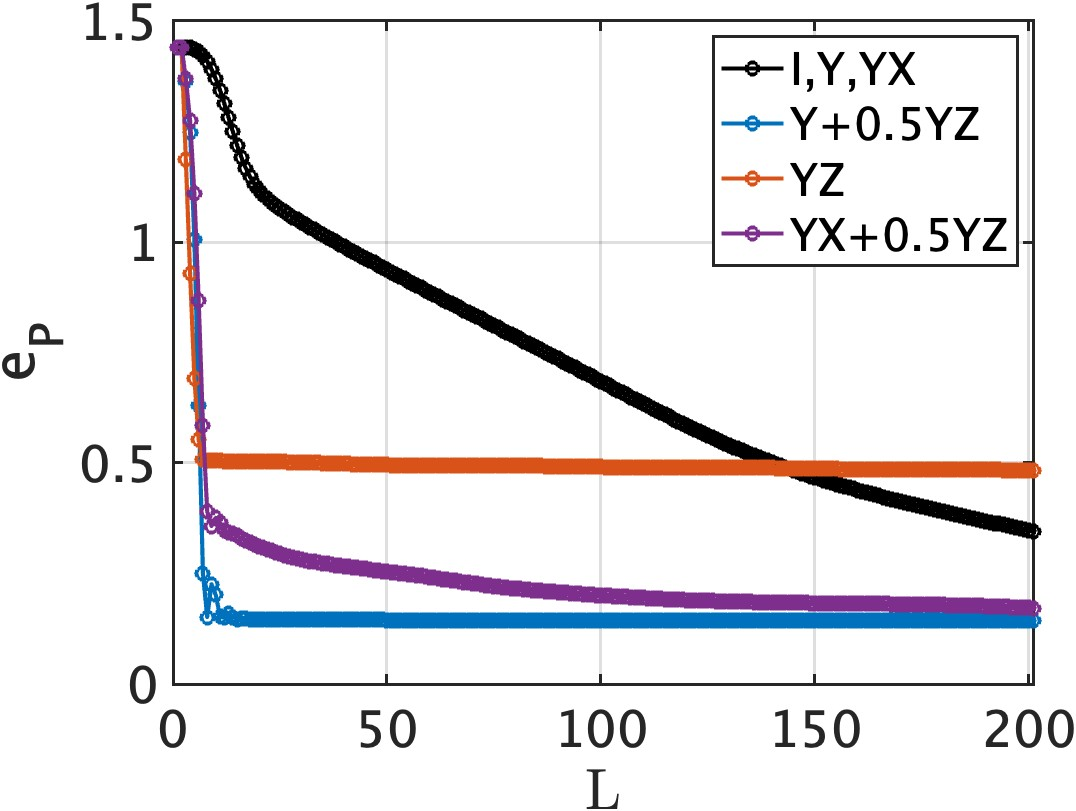
\includegraphics[scale=0.2,trim = 0in 1.6in 0in 0in,clip=true]{TFI1-04.jpg}} \\
    % \sidesubfloat[]{\label{:b}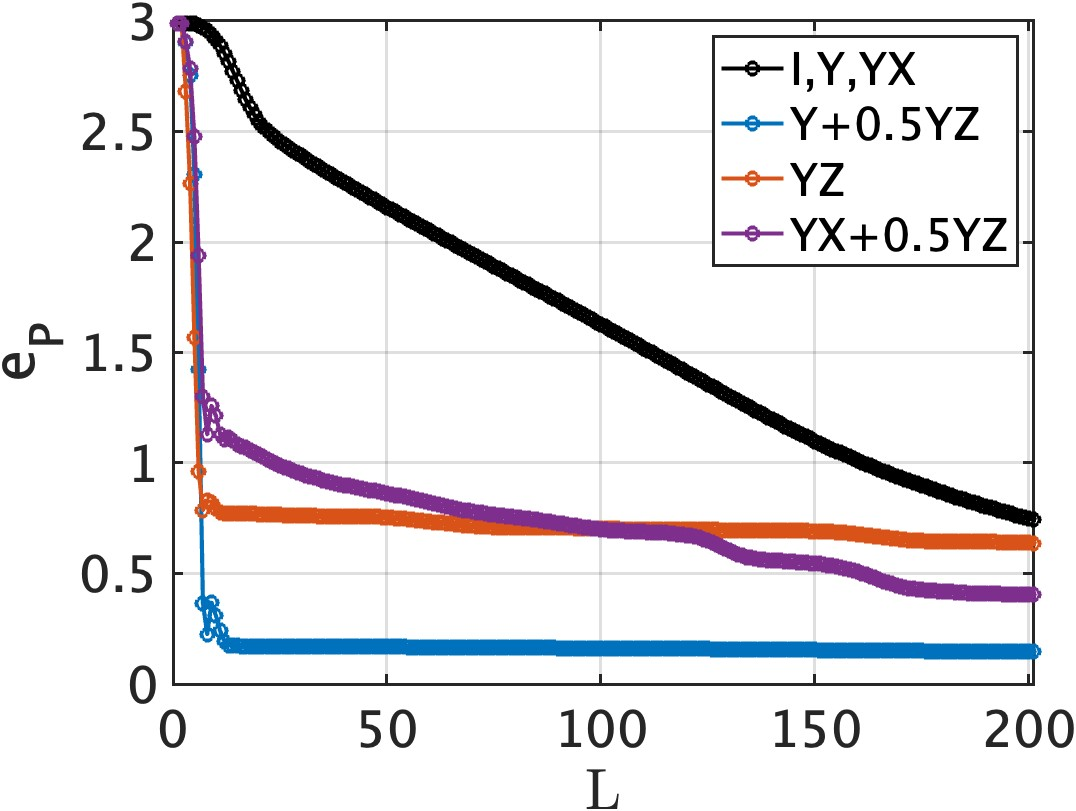
\includegraphics[scale=0.2,trim = 0in 1.6in 0in 0in,clip=true]{TFI1-14.jpg}} \\
    % \sidesubfloat[]{\label{:c}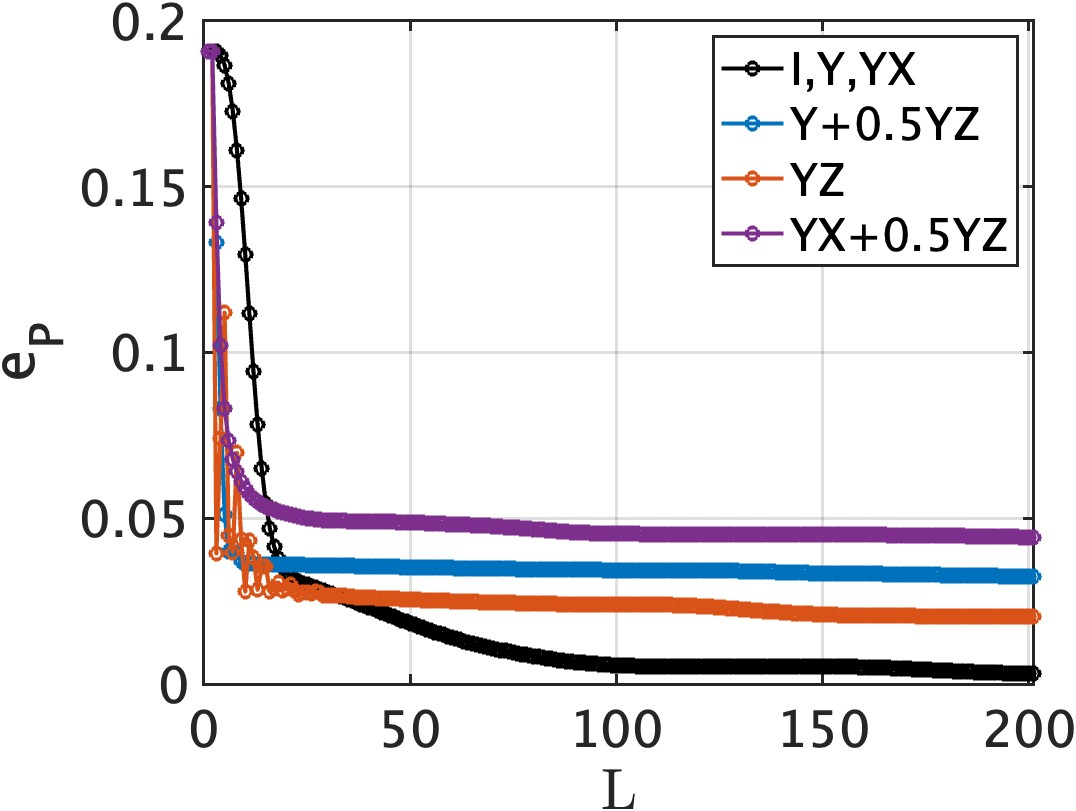
\includegraphics[scale=0.21]{TFI114.jpg}}
\caption{
   The CD-FQA protocol for additional cases for the TFI with
   $h_x$ = (a) $-0.4$, (b) $-1.4$,  (c) $1.4$.
}\label{fig:TFIappendix1}
\end{figure}


\begin{figure}[h!]
    \centering
    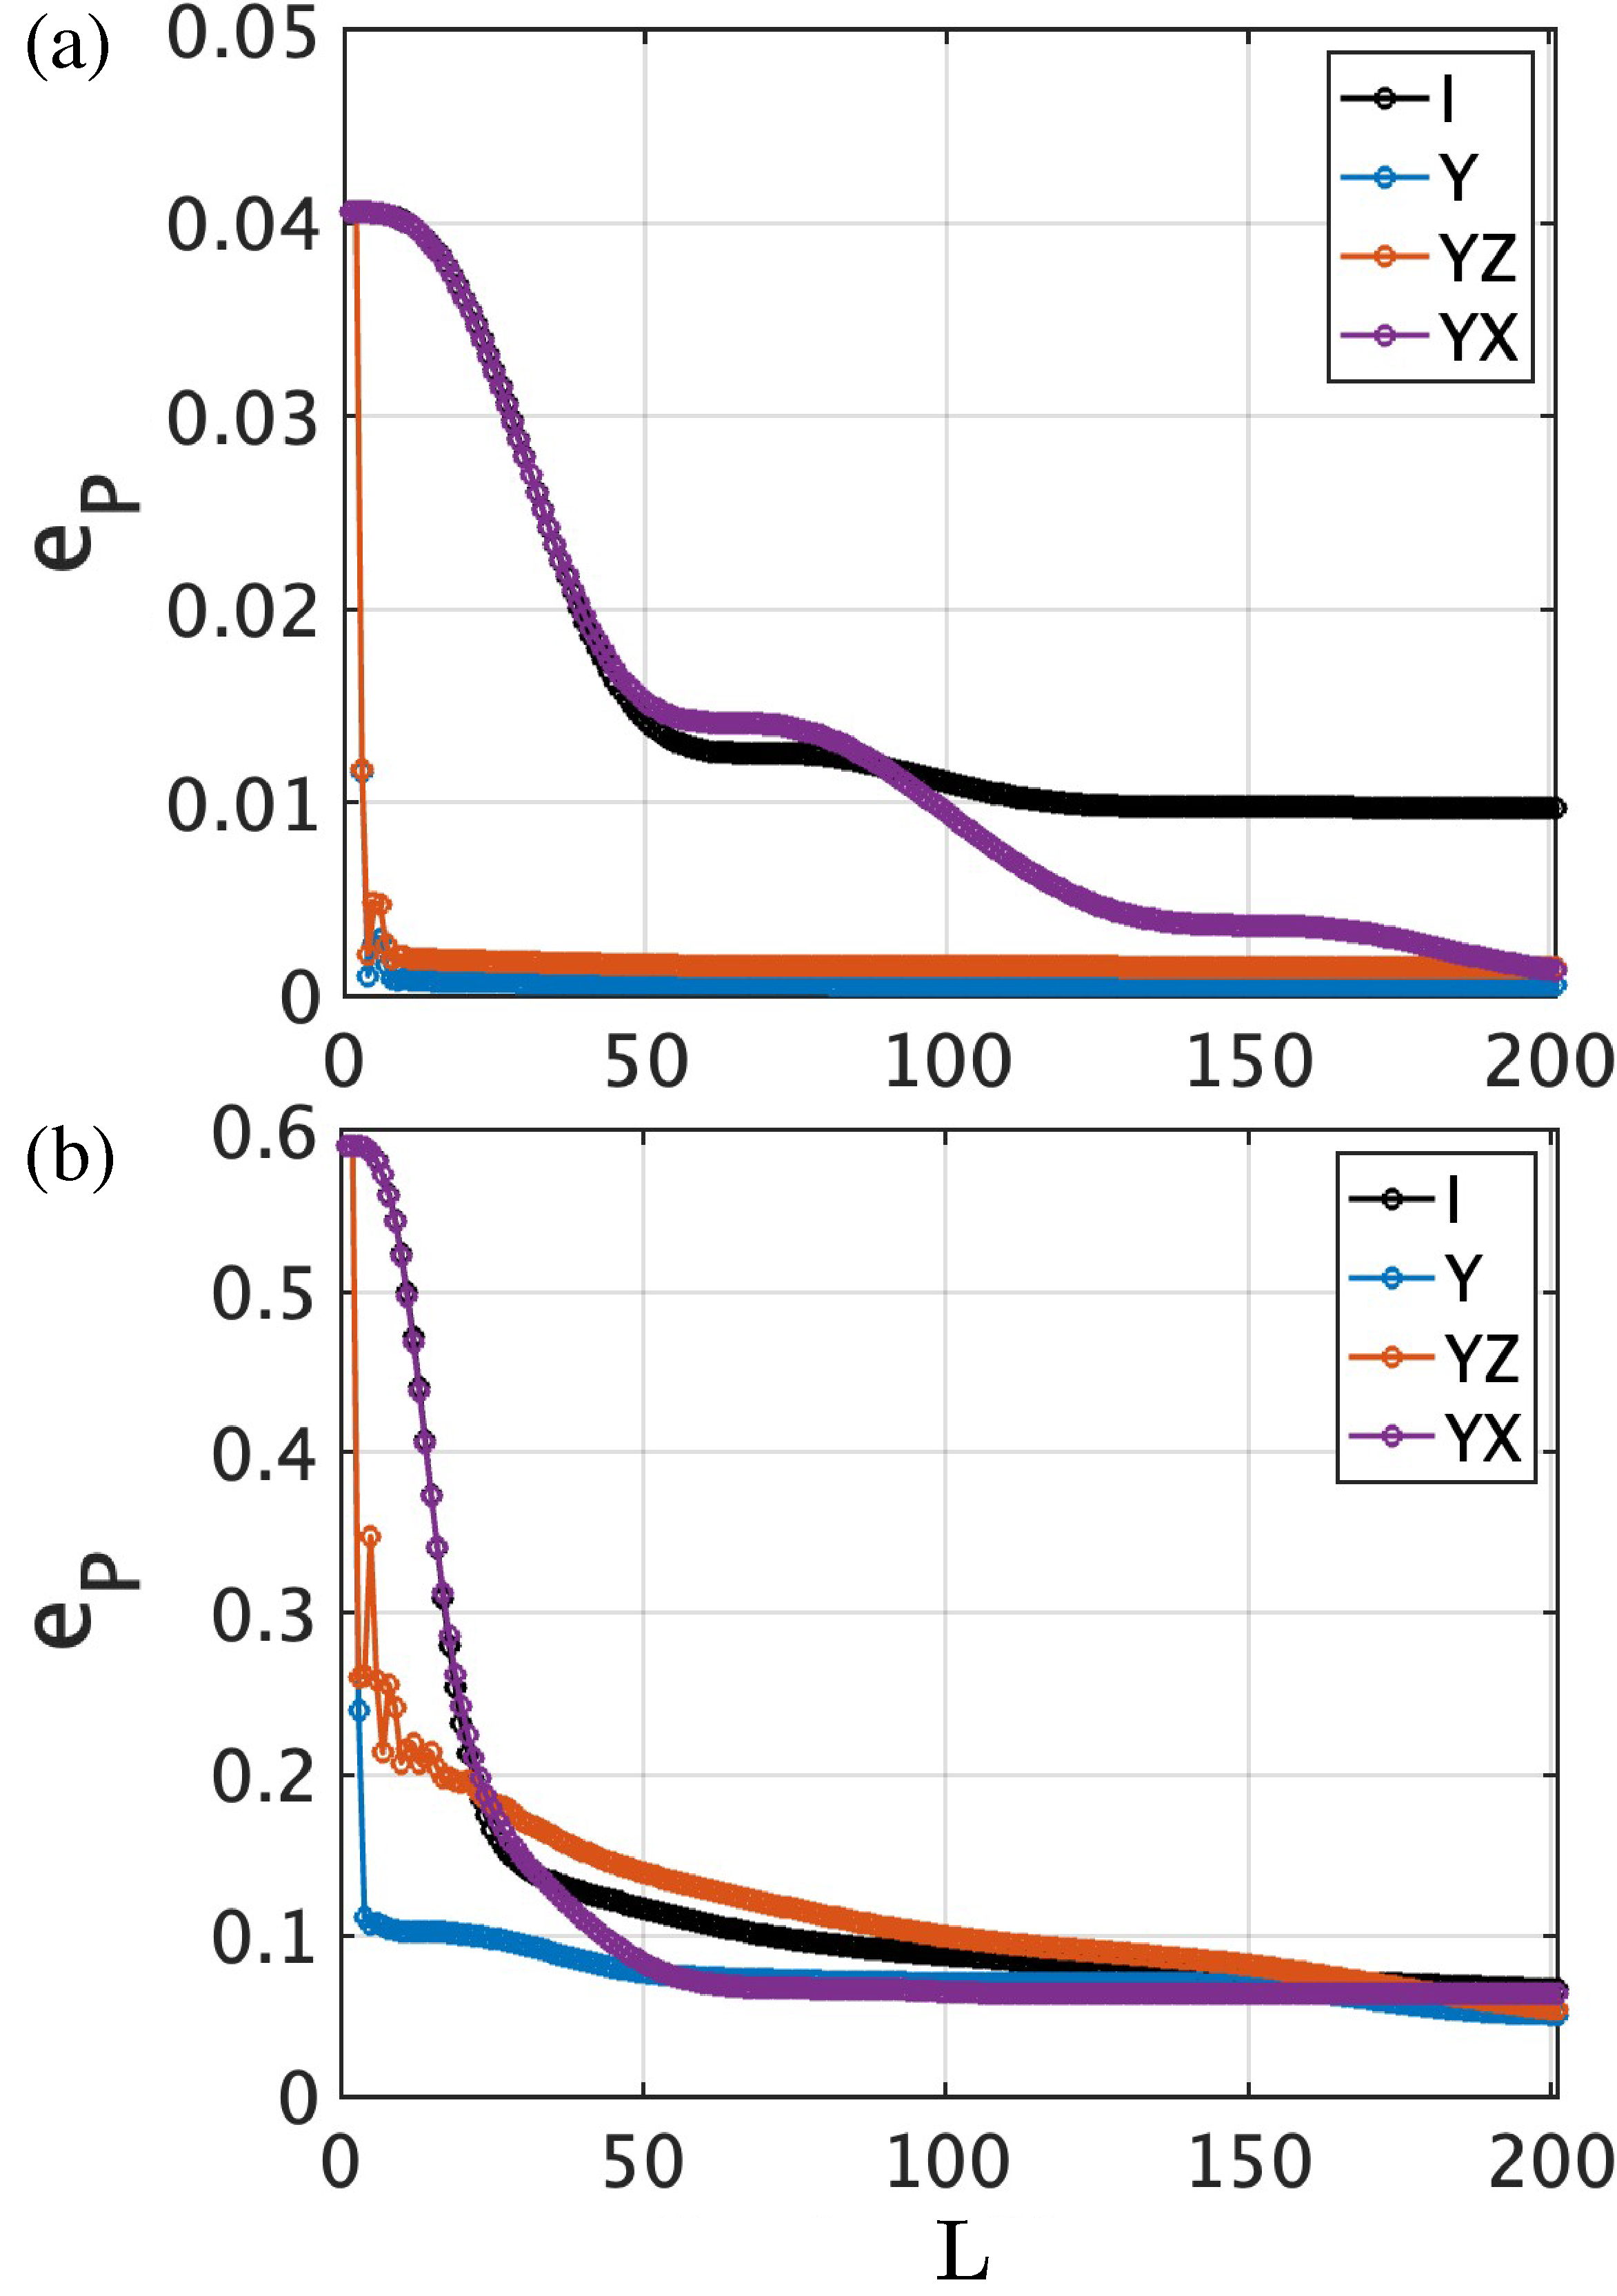
\includegraphics[scale=0.2]{zadd.pdf}
    % \sidesubfloat[]{\label{:a}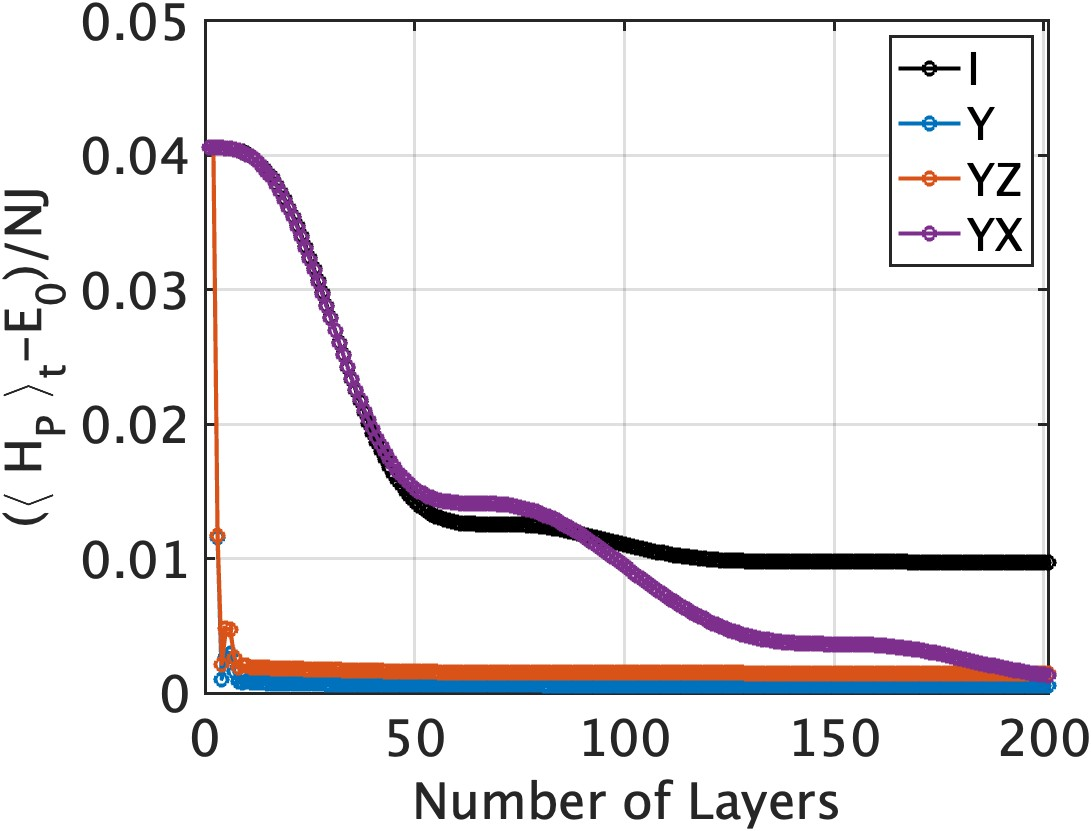
\includegraphics[scale=0.2,trim = 0in 1.6in 0in 0in,clip=true]{ZTFIM1004.jpg}}\\
    % \sidesubfloat[]{\label{:b}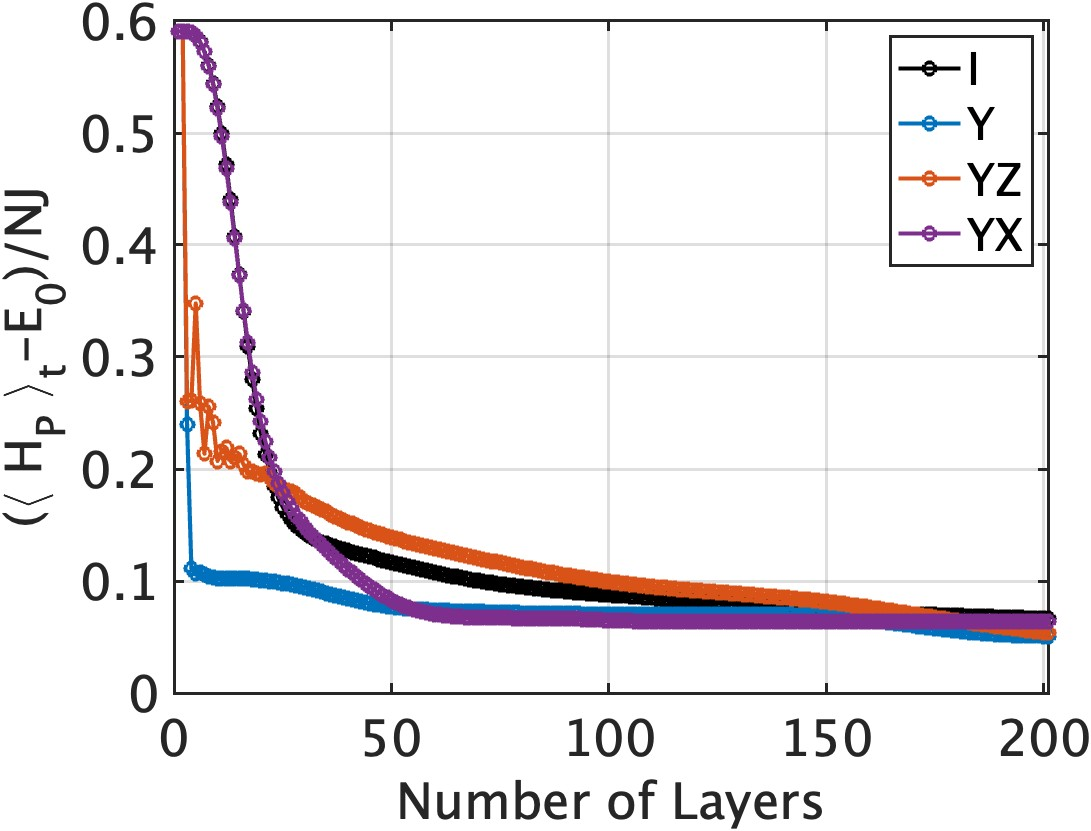
\includegraphics[scale=0.2]{ZTFIM1014.jpg}}
    \caption{The CD-FQA protocol for the TFI with alternate first control Hamiltonian $H_1=Z$ is shown for $h_x$ = (a) $0.4$, (b) $1.4$. The initial state is the ground state of $Z$.}
    \label{fig:TFIwithZ}
\end{figure}

\begin{figure}[h!]
    \centering
    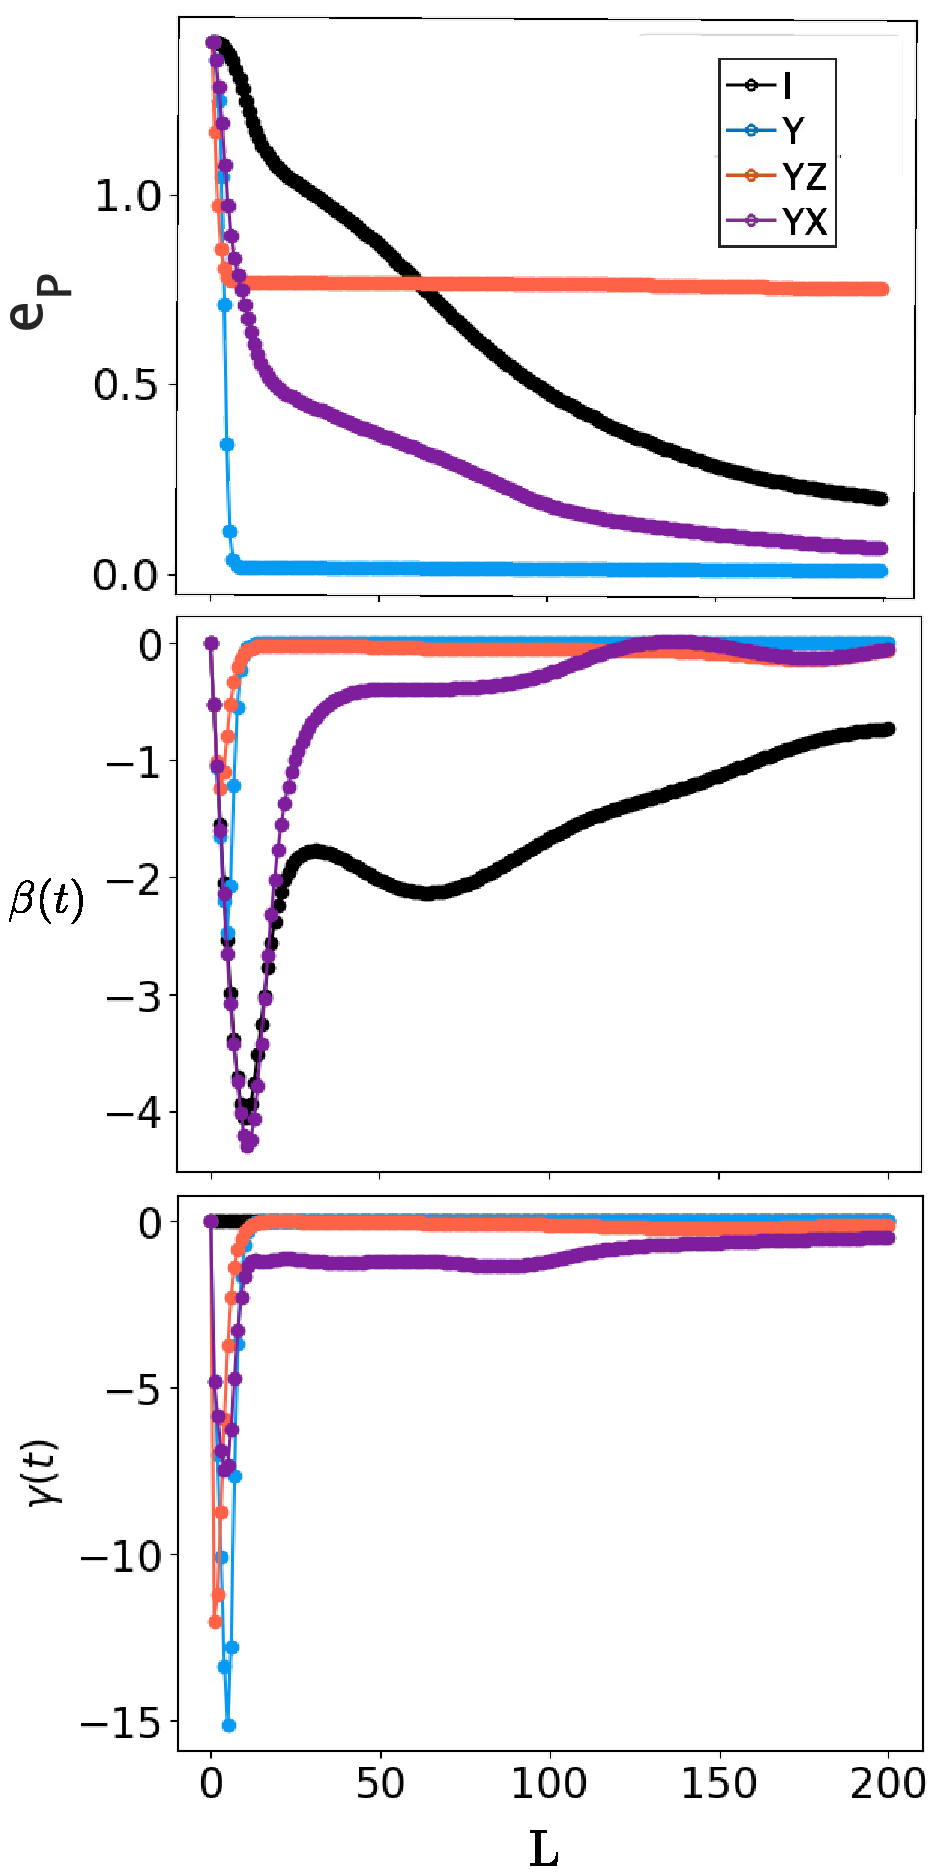
\includegraphics[scale=0.5]{pennylane_vf.pdf}
    % \sidesubfloat[]{\label{:a}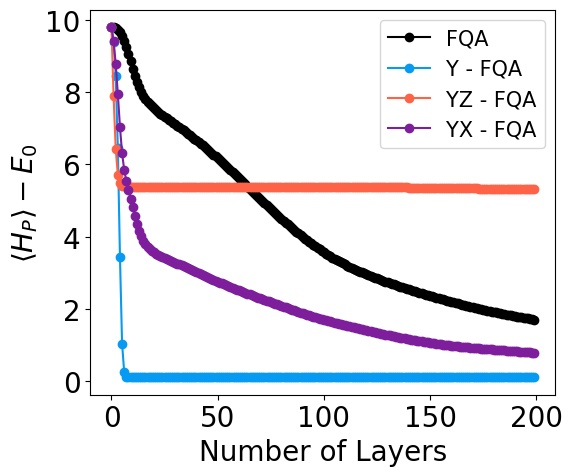
\includegraphics[scale=0.25]{PLLFIM1040.jpg}} \\
    % \sidesubfloat[]{\label{:b}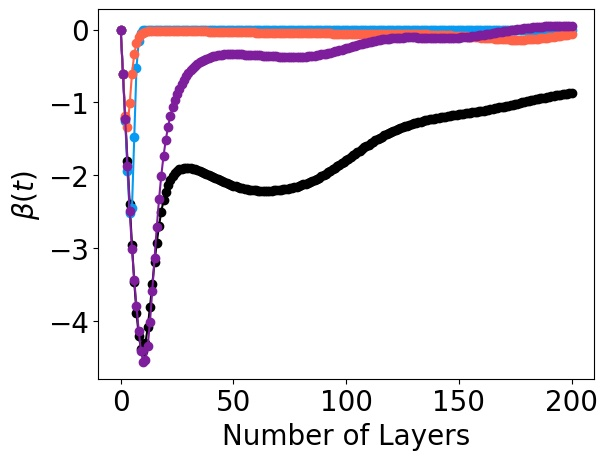
\includegraphics[scale=0.25]{PLLFIM1040_beta.jpg}}\\
    % \sidesubfloat[]{\label{:c}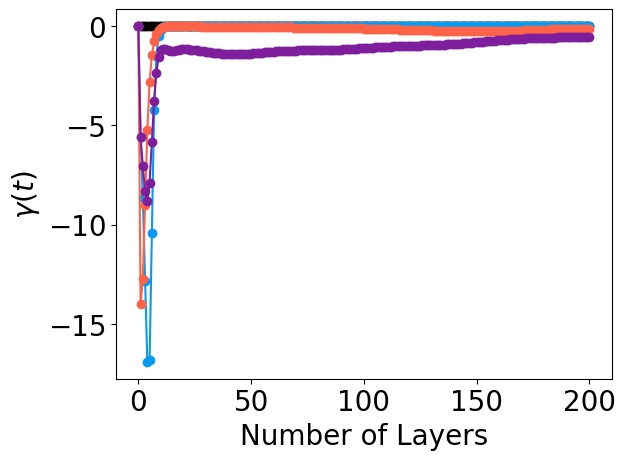
\includegraphics[scale=0.25]{PLLFIM1040_gamma.jpg}}
    \caption{FQA simulation results for LFI with $N=6$, $\Delta t = 0.01$, $\alpha=6$, and parameters $\{h_z,h_x\} = \{0.4,0.0\}$. The simulation was performed with PennyLane~\cite{bergholm2018pennylane}, where each unitary evolution is implemented with the first-order Trotter approximation. The result is consistent with the quasi-exact simulation without Trotterization presented in Fig.~\ref{fig:LFI}.}
    \label{fig:PLLFI}
\end{figure}

% \section{Convergence of CD-FQA across different system sizes} 
% \label{app:system-size}

% In this appendix, we present additional plots for MFI. In Fig.
% \ref{fig:L1000}a, we show the average energy as a function of
% the number of layers for three different system sizes up to 100
% layers and in Fig. \ref{fig:L1000}b the loglog plot is shown up
% to 1000 layers. As we increase the system sizes, the CD-FQA
% protocol and the stand FQA show slower convergence for larger
% system sizes except for the protocol with $Y$. This exception is
% detailed in the main text. The CD-FQA with $Y$ and \YX as the
% second control Hamiltonians exhibit convergence, while the
% protocol employing \YZ fails to converge even after 1000
% layers. The curves corresponding to protocols involving $Y$ and
% \YX consistently reside below the curve associated with the
% standard FQA, highlighting the superior performance of the
% CD-FQA protocol. 


% Figure \ref{fig:L1000}b highlights the CD-FQA dependency on the system size, where the average energy per site is plotted against the number of layers for various second control Hamiltonians for the MFI. As the system size increases, the CD-FQA demonstrates enhanced performance over smaller circuits while in larger circuits, the system with smaller size exhibits better convergence. This trend is evident in Fig. \ref{fig:L1000}b, where the curves for different system sizes intersect. A notable exception to this behavior is observed in the CD-FQA with $Y$, where the energies converge to a level of approximately $10^{-2}$ rapidly and the crossover does not occur. This observation suggests a subtle dependence of CD-FQA performance on both system size and control Hamiltonian. 
  


%RMK performed part of the work for this paper while visiting the Aspen Center for Physics, a center supported by the National Science Foundation under grant PHY-2210452.

% \begin{figure}
%     \centering  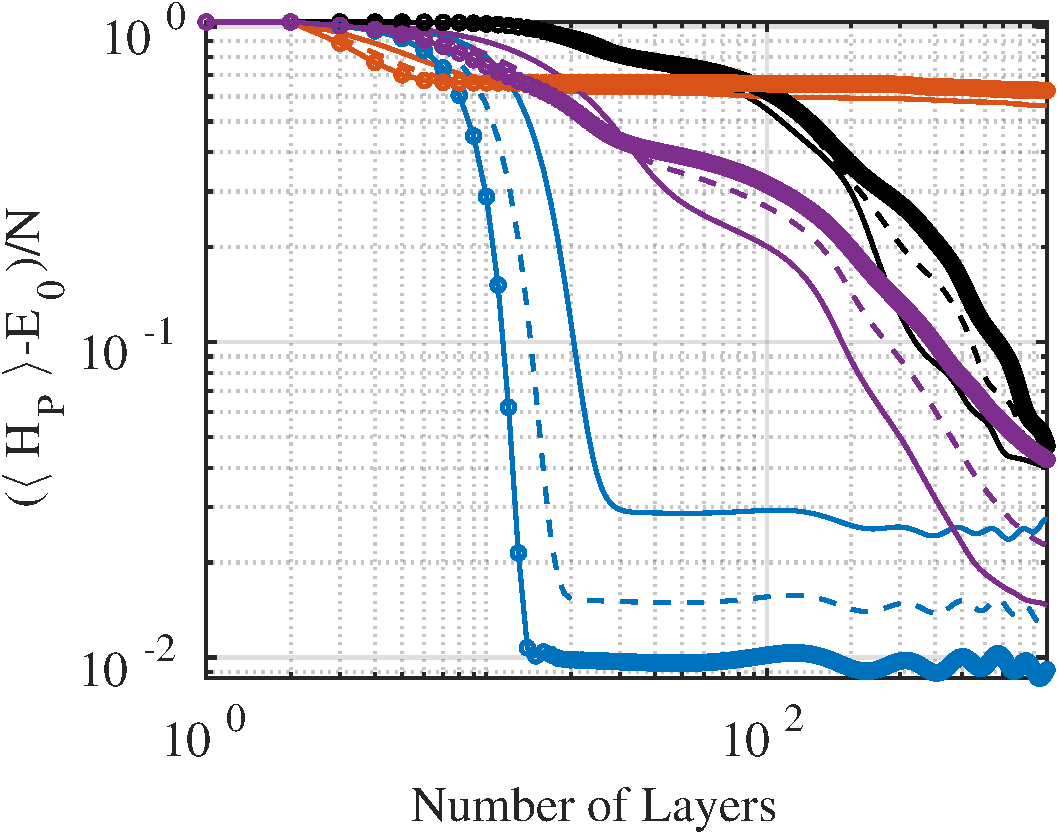
\includegraphics[scale=0.4]{MFIM1004systemsize.pdf}
%     \caption{The CD-FQA protocol is shown for the MFI for three different system sizes. All the other parameters are the same as in Fig. \ref{fig:MFI}}
%     \label{fig:differentsize}
% \end{figure}



\section{CD-FQA for the TFI: additional plots}

In this appendix, we introduce additional plots that extend the
analysis of the TFI model with variations in parameters. Fig.~\ref{fig:TFIappendix1} provides insights into the performance of
the CD-FQA across three TFI models characterized by distinct
parameter sets, $h_x=-0.4$, $-1.4$, and $1.4$. For the case of
$h_x=-0.4$, the ground state is in a antiferromagnetic phase.
The performance of CD-FQA protocol is similar to that shown in
Fig. \ref{fig:TFI} in the main text. When the $|h_x|>1$, the
spins in the ground state are more likely to be aligned along
x-axis. Therefore, the \YX operator does not play any
significant role compared to the \YZ operator, see Figs.~\ref{fig:TFIappendix1}b,c. Finally,  when $h_x>1$, the ground
state is close to the initial state and therefore we see a fast
convergence using the standard FQA. 

In Fig.~\ref{fig:TFIwithZ}, we apply the CD-FQA protocol to
two TFI models where $H_1=Z$ serves as the first control
Hamiltonian, coupled with the initial state
$|\psi_0\ra=|\uparrow \uparrow ...\uparrow\ra$. Unlike the
results observed in Fig. \ref{fig:TFI}, where the CD-FQA with
$Y$ and \YX aligns with the standard FQA, the CD-FQA protocols
in Fig. \ref{fig:TFIwithZ} yield different curves for the
average energy. The contrast between the two figures underscores
the significant impact of the first control Hamiltonian on the
overall performance of the algorithm. In the context of the TFI
model, the choice of $Z$ as the first control Hamiltonian tends
to be more effective than opting for $X$. 


\section{Simulation on PennyLane} 

In the main text, simulation results were presented for
unitaries without Trotterization. However, in practical quantum
devices, it is common practice to execute unitary (time)
evolutions using the Trotter approximation. In this appendix, we
showcase a classical simulation conducted through the
application of Pennylane tools in the first-order Trotter
approximation, as illustrated in Fig.~\ref{fig:PLLFI}. For
demonstration purposes, we choose the LFI model, and the plots
affirm the consistency of the curves with the results previously
depicted in Fig.~\ref{fig:LFI}.


\bibliographystyle{apsrev4-1}
%\bibliographystyle{jabbrv_vancouver}
\bibliography{bib}


\end{document}



% Figure 1:
% \begin{itemize}
%     \item J=1,hz=0.4,hx=0.4
% \end{itemize}

% Figure 2:
% \begin{itemize}
%     \item J=1,hz=0.4,hx=0
% \end{itemize}

% Figure 3:
% \begin{itemize}
%     \item J=1,hz=0,hx=0.4
%     \item J=1,hz=0,hx=-0.4
% \end{itemize}

% Figure 4:
% \begin{itemize}
%     \item J=1,hz=0,hx=0
% \end{itemize}

% All figures must contain 3 curves (FALQON, Y-FALQON, YZ-FALQON) and a reference line for ground state energy

% \section{Improving CD-FALQON using time-dependent perturbation}
% Figure 5: Include perturbation
% \begin{itemize}
%     \item J=1,hz=0,hx=0
% \end{itemize}

% \section{Experiment in IBM}
% Figure 6: Same as Figure 1 but in quantum circuit
% \begin{itemize}
%     \item J=1,hz=0,hx=0
% \end{itemize}

% Figure 7: Same as Figure 5 but in quantum circuit
% \begin{itemize}
%     \item J=1,hz=0,hx=0
% \end{itemize}
% \section{Ising spin models}

% Figure~\ref{fig:FALQON-CD-Mixed-Ising}.

% % \begin{figure*}
% %     \subfloat[]{\label{fig:MFI-100000}\includegraphics[width=.40\textwidth]{J10hz00hx00.pdf}}
% %     \hfill
% %     \subfloat[]{\label{fig:MFI-100400}\includegraphics[width=.40\textwidth]{J10hz04hx00.pdf}}
% %     \hfill
% %     \subfloat[]{\label{fig:MFI-100004}\includegraphics[width=.40\textwidth]{J10hz00hx04.pdf}}
% %     \hfill
% %     \subfloat[]{\label{fig:MFI-100404}\includegraphics[width=.40\textwidth]{J10hz04hx04.pdf}}
% %     \caption{Counterdiabatic-inspired FALQON algorithm for the mixed-field Ising model.}
% %   \label{fig:FALQON-CD-Mixed-Ising}
% % \end{figure*}

% \subsection{Integrable model}
% \subsection{Nonintegrable model}


% \section{Lipkin-Meshkov-Glick model}

% Figure~\ref{fig:FALQON-CD-LMG}
% \begin{figure}
%     \includegraphics[width=0.5\textwidth]{LMGJ10h04.pdf}
%     \caption{Counterdiabatic-inspired FALQON algorithm for the LMG model.}
%     \label{fig:FALQON-CD-LMG}
% \end{figure}


% We propose that additional control parameters can be constructed from a counterdiabaticity-inspired approach to accelerate the ground state preparation. Let us denote this ``new" Hamiltonian as $H_{\rm CD}$.



% \begin{figure}
%     \centering
%     \sidesubfloat[]{\label{:a}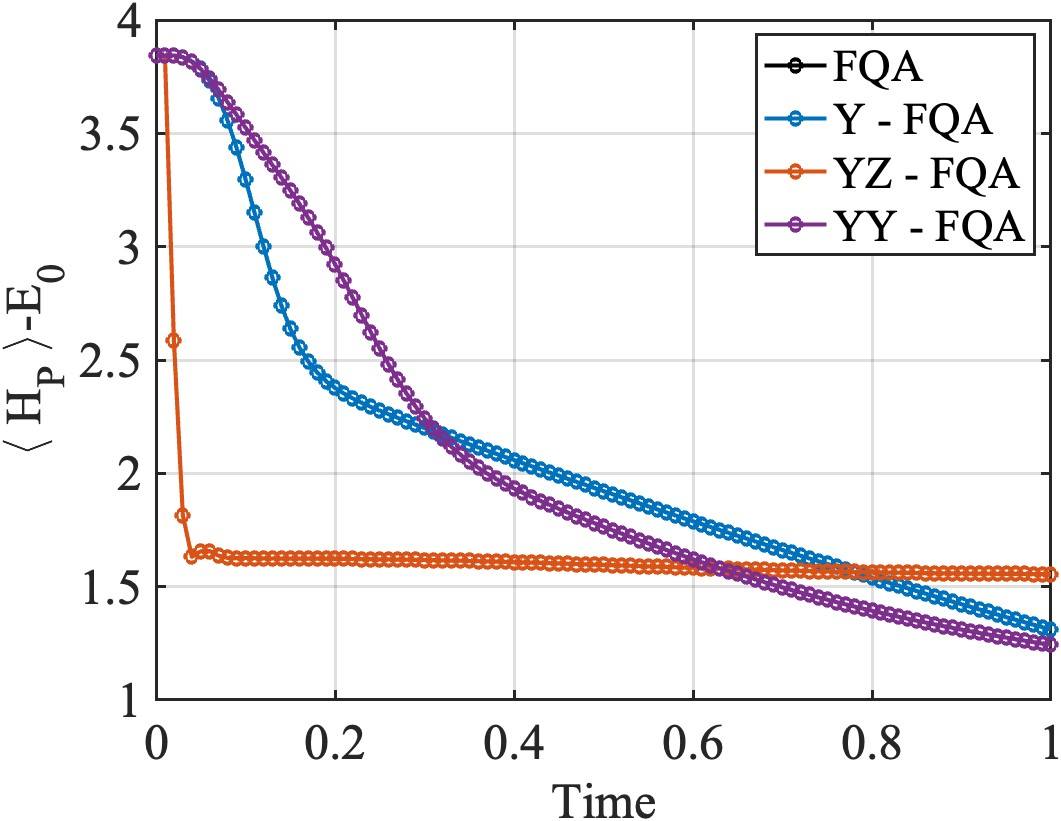
\includegraphics[scale=0.165]{TFIM-1004.jpg}} \\
%     \sidesubfloat[]{\label{:b}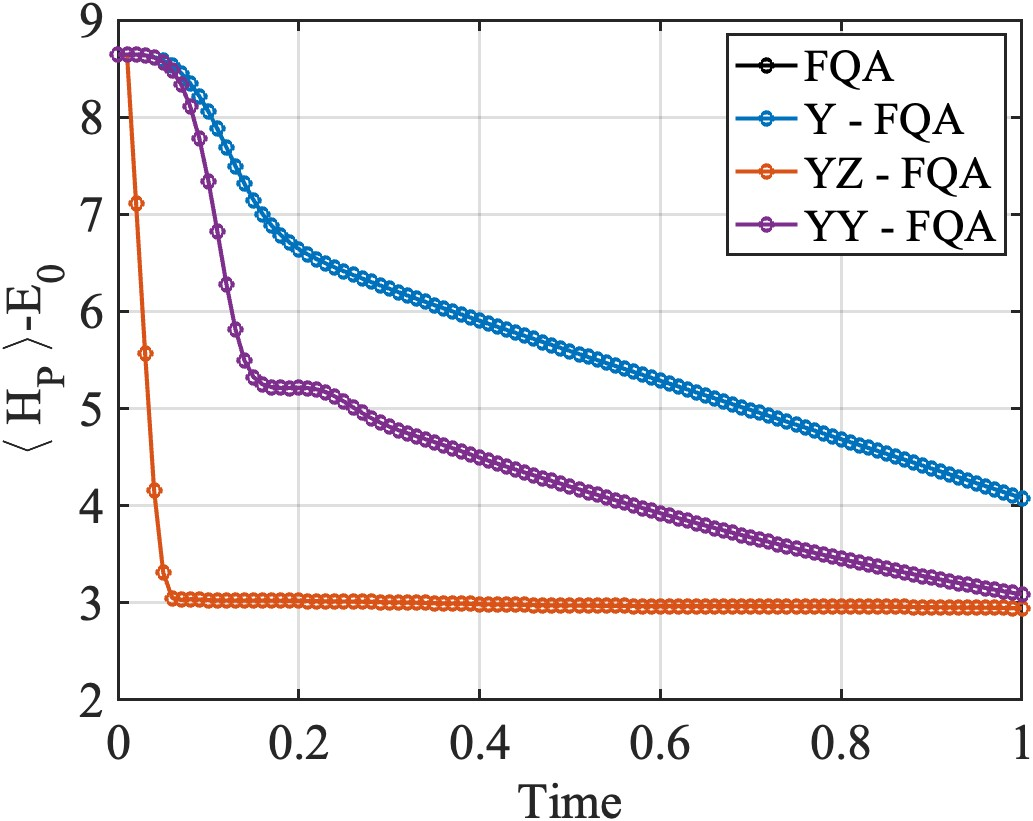
\includegraphics[scale=0.165]{TFIM-10-04.jpg}}\\
%     \sidesubfloat[]{\label{:a}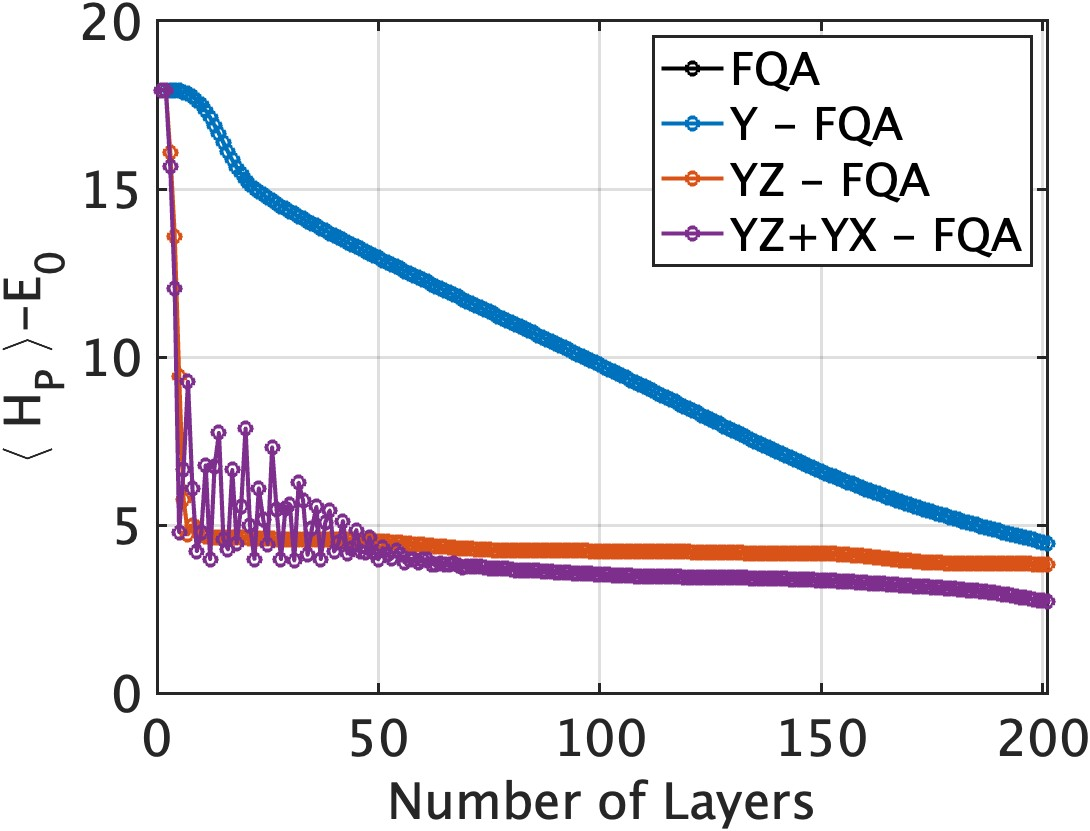
\includegraphics[scale=0.165]{TFIM-1014.jpg}} \\
%     \sidesubfloat[]{\label{:b}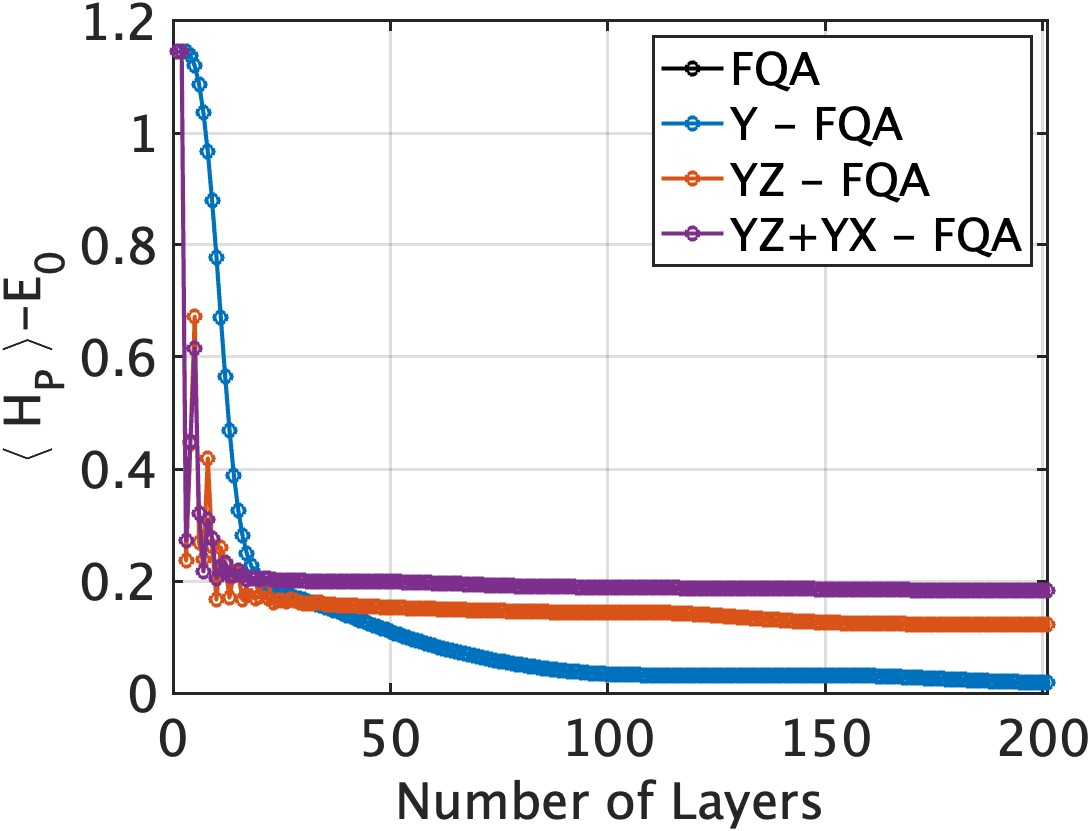
\includegraphics[scale=0.165]{TFIM-10-14.jpg}}\\
%     \caption{(a) LFI (b) MFI}
%     \label{fig:enter-label}
% \end{figure}
% \vspace{100mm}
% \begin{figure}
%     \centering
%     \sidesubfloat[]{\label{:a}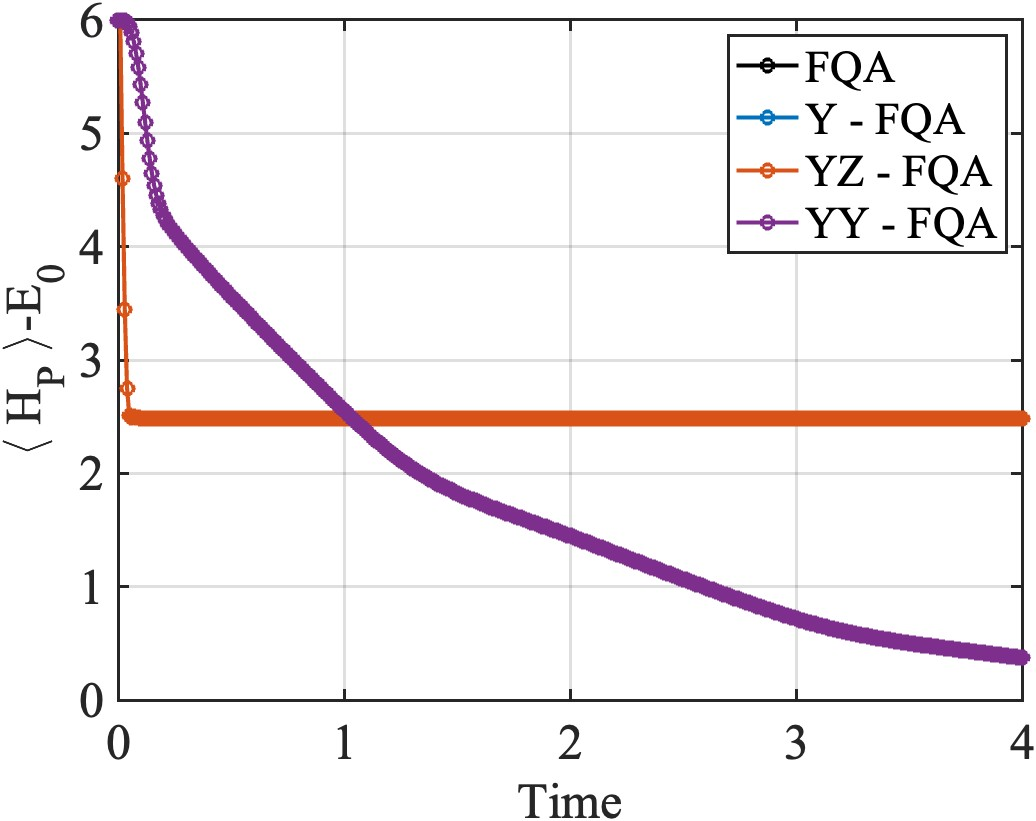
\includegraphics[scale=0.165]{GHZ-100.jpg}}
%     \caption{(a) GHZ}
%     \label{fig:enter-label}
% \end{figure}
% Counterdiabatic driving is a concept in time-dependent quantum evolution
